%
% $Id: tutorial.tex,v 1.11.2.1 2012/02/26 01:06:26 sfeam Exp $
%
% Tutorial for gnuplot plotting program, for LaTeX users
% David Kotz
% Duke University Computer Science Department
%
% Slightly updated by the gnuplot team in 2004, for gnuplot 4.0.
% Updated for gnuplot 4.2 to include epslatex example by Ethan A Merritt
% Updated for gnuplot 4.4 to replace 'set size' with 'set term latex size'
% Updated for gnuplot 4.6 to mention the newer TeX-based terminals
%
% NOTE: If LaTeX runs out of memory processing plots,
% add ``with lines 4'' to each curve in eg*.plt and rerun make.
%

% some header info
% 
% Header file for tutorial.tex
%

% Spacing
\newcommand{\singlespace}
  {\addtolength{\baselineskip}{-.333\baselineskip}}
\newcommand{\doublespace}
  {\addtolength{\baselineskip}{.5\baselineskip}}

% Spacing for the whole document 
\newcommand{\currentspace}{} % use this for single space
% \newcommand{\currentspace}{\doubleespace} % use this for double space

% Common abbreviations
% (Remember to put '\ ' after if an interword space is
%  desired rather than end-of-sentence space. Same for '.etc)' ).
\newcommand{\eg}{{\em e.g.}}		% e.g.
\newcommand{\ie}{{\em i.e.}}		% i.e.
\newcommand{\etc}{{\em etc.}}		% etc.
\newcommand{\vs}{{\em vs.}}		% vs.
\newcommand{\usec}{{$\mu$}sec}	% microseconds

% \boxfigure{pos}{wid}{text}:  A figure with a box around it
%
% pos	the usual figure placement arg: eg. htbp
% wid	the width of the figure, in some units: eg. 5in
% text	the contents of the figure, including picture/caption/label/etc
%
\newlength{\boxwidth}
\newcommand{\boxfigure}[3]{
	\begin{figure}[#1]
		\setlength{\boxwidth}{#2}
		\addtolength{\boxwidth}{.1in}

		\centering
		\framebox[\boxwidth]{
			\begin{minipage}{#2}
			#3
			\end{minipage}
		}
	\end{figure}  
}

% use \fullboxwidth for arg 2 of boxfigure to get box of size \textwidth

% To show a syntax for a gnutex command
\newenvironment{syntax}{\begin{quote}\tt}{\end{quote}}

\ifx\LaTeXe\undefined
% old LaTeX version
% add `,a4' to `toc_entry' to load settings for A4-paper
% see below if you add 11pt or 12pt
\documentstyle[titlepage,a4]{article}
\else
% LaTeX2e version
% add `[a4paper]' before `{article}' to load settings for A4-paper
% see below if you add 11pt or 12pt
\documentclass[titlepage,a4paper]{article} % DSL 24 May 1995
\usepackage{latexsym}
\usepackage{amssymb}
% If you are concerned about
% LaTeX Warning: \oval, \circle, or \line size unavailable on input line
% warnings, uncomment one of the following lines. You'll need to create
% tutorial.ps then.
%\usepackage{eepic}
%\usepackage{pspicture}
\fi

% Other packages
\usepackage{url}

% Only needed for epslatex driver
\usepackage{graphicx}
\usepackage{color}

% Margins
\sloppy
\setlength{\textwidth}{6.5in}
\setlength{\textheight}{9in}
\setlength{\topmargin}{-0.5in}
\setlength{\oddsidemargin}{0pt}
\setlength{\evensidemargin}{0pt}

% see above
\newlength{\fullboxwidth}
\setlength{\fullboxwidth}{\textwidth}
\addtolength{\fullboxwidth}{-0.1in}




\begin{document}


\begin{titlepage}

\begin{center}
{\Large \bf \LaTeX\ and the Gnuplot Plotting Program}

\vskip2cm

{\bf David Kotz} \\[0.4cm]
Principal author of this tutorial for gnuplot 3.0, July 3, 1991 \\[1.0cm]

{\bf current gnuplot team} \\[0.4cm]
Updates of this tutorial for gnuplot 4.0, March 2004 \\
Update of this tutorial for gnuplot 4.2, August 2006 \\
Update of this tutorial for gnuplot 4.4, September 2010 \\
Update of this tutorial for gnuplot 4.6, February 2012

\vskip2cm

% All plots in this document were made with the current version of gnuplot.

\end{center}

\vfil
\vfil
\tableofcontents
\vfil

\end{titlepage}


\pagestyle{myheadings}
\markright{Gnuplot \LaTeX\ Tutorial Version 4.6}

\currentspace % defined in header.tex

\section{Introduction and History}

Gnuplot was originally developed by Colin Kelley and Thomas Williams
in 1986 to plot functions and data files on a variety of terminals.
In 1988 and 1989 I created an alternate version, known as Gnu\TeX,
that supported a new ``terminal type'' called {\tt latex}, so gnuplot
would output \LaTeX\ code. The plot could then be included in a
\LaTeX\ document. I added a number of embellishments, supported only
by the {\tt latex} terminal, allowing the user to produce
publication-quality plots.

In late 1989 and early 1990 Gnu\TeX\ and a number of other gnuplot
variants were merged together into a new release of gnuplot, 2.0. This
includes, among many other improvements, a \LaTeX\ driver derived from
the one in Gnu\TeX.
Anyone interested in using gnuplot with \LaTeX\ should read the next
section, a tutorial, and the primary gnuplot manual.

The reader should note that the \LaTeX\ picture environments output by
gnuplot can be quite large and complicated, and can easily exceed the
memory capacity of \TeX. If an enlarged version of \TeX\ is available,
it is wise to use it. Otherwise, keep your plots simple and add
\verb+\clearpage+ to your document where necessary.

There is also an EEPIC driver ({\tt eepic}), intended for use with
the EEPIC macro package for \LaTeX. EEPIC allows for much more
efficient line-drawing, runs through \LaTeX\ faster, and uses less
memory.  See Section~\ref{s:eepic} for more information.

Other gnuplot terminal types have been added that take advantage of
newer \TeX\ and \LaTeX\ packages and variants, including {\tt emtex}, 
{\tt metafont}, {\tt epslatex}, {\tt tikz}, and {\tt context}.

\section{Using gnuplot for \LaTeX: a Tutorial}

Gnuplot is by nature an interactive program. Users making plots for
\LaTeX\ will generally not use gnuplot interactively.  Whenever hard
copy is desired from gnuplot, the program need not be run on a
graphics terminal. In this case the output is directed to a file or
pipe, then sent to the appropriate output device.

We now ignore the interactive nature of gnuplot and provide the input
to gnuplot from a file, \ie,
\begin{verbatim}
      gnuplot plotcommands.gp
\end{verbatim}
In this example, all of the commands to gnuplot are contained in the
file {\tt plotcommands.gp}. Multiple filenames may be supplied to gnuplot
this way, read in the order they are given.  The output (one or more
plots) may be piped to another program or redirected to a file.
Usually, however, we direct the output explicitly with an instruction
to gnuplot (the {\tt set output "outfile.tex"} command). Gnuplot continues to
print error messages to the terminal (stderr). After printing, the output file
has to be closed by {\tt set output}, \ie{} without the file name specification.

\paragraph{Example 1:} Here is a first example, producing a plot for
this document. The gnuplot input file is given below, and the output
appears as Figure~\ref{eg1}. The input file defines the output to be
in \LaTeX, gives a file name for the output, and plots $y=\sin(x)$ for
$x$ on $[-\pi,\pi]$. To produce the figure, I simply
\verb+% GNUPLOT: LaTeX picture
\setlength{\unitlength}{0.240900pt}
\ifx\plotpoint\undefined\newsavebox{\plotpoint}\fi
\sbox{\plotpoint}{\rule[-0.200pt]{0.400pt}{0.400pt}}%
\begin{picture}(1500,900)(0,0)
\sbox{\plotpoint}{\rule[-0.200pt]{0.400pt}{0.400pt}}%
\put(150.0,82.0){\rule[-0.200pt]{4.818pt}{0.400pt}}
\put(130,82){\makebox(0,0)[r]{-1}}
\put(1429.0,82.0){\rule[-0.200pt]{4.818pt}{0.400pt}}
\put(150.0,160.0){\rule[-0.200pt]{4.818pt}{0.400pt}}
\put(130,160){\makebox(0,0)[r]{-0.8}}
\put(1429.0,160.0){\rule[-0.200pt]{4.818pt}{0.400pt}}
\put(150.0,237.0){\rule[-0.200pt]{4.818pt}{0.400pt}}
\put(130,237){\makebox(0,0)[r]{-0.6}}
\put(1429.0,237.0){\rule[-0.200pt]{4.818pt}{0.400pt}}
\put(150.0,315.0){\rule[-0.200pt]{4.818pt}{0.400pt}}
\put(130,315){\makebox(0,0)[r]{-0.4}}
\put(1429.0,315.0){\rule[-0.200pt]{4.818pt}{0.400pt}}
\put(150.0,393.0){\rule[-0.200pt]{4.818pt}{0.400pt}}
\put(130,393){\makebox(0,0)[r]{-0.2}}
\put(1429.0,393.0){\rule[-0.200pt]{4.818pt}{0.400pt}}
\put(150.0,471.0){\rule[-0.200pt]{4.818pt}{0.400pt}}
\put(130,471){\makebox(0,0)[r]{ 0}}
\put(1429.0,471.0){\rule[-0.200pt]{4.818pt}{0.400pt}}
\put(150.0,548.0){\rule[-0.200pt]{4.818pt}{0.400pt}}
\put(130,548){\makebox(0,0)[r]{ 0.2}}
\put(1429.0,548.0){\rule[-0.200pt]{4.818pt}{0.400pt}}
\put(150.0,626.0){\rule[-0.200pt]{4.818pt}{0.400pt}}
\put(130,626){\makebox(0,0)[r]{ 0.4}}
\put(1429.0,626.0){\rule[-0.200pt]{4.818pt}{0.400pt}}
\put(150.0,704.0){\rule[-0.200pt]{4.818pt}{0.400pt}}
\put(130,704){\makebox(0,0)[r]{ 0.6}}
\put(1429.0,704.0){\rule[-0.200pt]{4.818pt}{0.400pt}}
\put(150.0,781.0){\rule[-0.200pt]{4.818pt}{0.400pt}}
\put(130,781){\makebox(0,0)[r]{ 0.8}}
\put(1429.0,781.0){\rule[-0.200pt]{4.818pt}{0.400pt}}
\put(150.0,859.0){\rule[-0.200pt]{4.818pt}{0.400pt}}
\put(130,859){\makebox(0,0)[r]{ 1}}
\put(1429.0,859.0){\rule[-0.200pt]{4.818pt}{0.400pt}}
\put(179.0,82.0){\rule[-0.200pt]{0.400pt}{4.818pt}}
\put(179,41){\makebox(0,0){-3}}
\put(179.0,839.0){\rule[-0.200pt]{0.400pt}{4.818pt}}
\put(386.0,82.0){\rule[-0.200pt]{0.400pt}{4.818pt}}
\put(386,41){\makebox(0,0){-2}}
\put(386.0,839.0){\rule[-0.200pt]{0.400pt}{4.818pt}}
\put(593.0,82.0){\rule[-0.200pt]{0.400pt}{4.818pt}}
\put(593,41){\makebox(0,0){-1}}
\put(593.0,839.0){\rule[-0.200pt]{0.400pt}{4.818pt}}
\put(800.0,82.0){\rule[-0.200pt]{0.400pt}{4.818pt}}
\put(800,41){\makebox(0,0){ 0}}
\put(800.0,839.0){\rule[-0.200pt]{0.400pt}{4.818pt}}
\put(1006.0,82.0){\rule[-0.200pt]{0.400pt}{4.818pt}}
\put(1006,41){\makebox(0,0){ 1}}
\put(1006.0,839.0){\rule[-0.200pt]{0.400pt}{4.818pt}}
\put(1213.0,82.0){\rule[-0.200pt]{0.400pt}{4.818pt}}
\put(1213,41){\makebox(0,0){ 2}}
\put(1213.0,839.0){\rule[-0.200pt]{0.400pt}{4.818pt}}
\put(1420.0,82.0){\rule[-0.200pt]{0.400pt}{4.818pt}}
\put(1420,41){\makebox(0,0){ 3}}
\put(1420.0,839.0){\rule[-0.200pt]{0.400pt}{4.818pt}}
\put(150.0,82.0){\rule[-0.200pt]{0.400pt}{187.179pt}}
\put(150.0,82.0){\rule[-0.200pt]{312.929pt}{0.400pt}}
\put(1449.0,82.0){\rule[-0.200pt]{0.400pt}{187.179pt}}
\put(150.0,859.0){\rule[-0.200pt]{312.929pt}{0.400pt}}
\put(1289,819){\makebox(0,0)[r]{sin(x)}}
\put(1309.0,819.0){\rule[-0.200pt]{24.090pt}{0.400pt}}
\put(150,470){\usebox{\plotpoint}}
\multiput(150.58,466.39)(0.493,-0.972){23}{\rule{0.119pt}{0.869pt}}
\multiput(149.17,468.20)(13.000,-23.196){2}{\rule{0.400pt}{0.435pt}}
\multiput(163.58,441.52)(0.493,-0.933){23}{\rule{0.119pt}{0.838pt}}
\multiput(162.17,443.26)(13.000,-22.260){2}{\rule{0.400pt}{0.419pt}}
\multiput(176.58,417.39)(0.493,-0.972){23}{\rule{0.119pt}{0.869pt}}
\multiput(175.17,419.20)(13.000,-23.196){2}{\rule{0.400pt}{0.435pt}}
\multiput(189.58,392.52)(0.493,-0.933){23}{\rule{0.119pt}{0.838pt}}
\multiput(188.17,394.26)(13.000,-22.260){2}{\rule{0.400pt}{0.419pt}}
\multiput(202.58,368.86)(0.494,-0.827){25}{\rule{0.119pt}{0.757pt}}
\multiput(201.17,370.43)(14.000,-21.429){2}{\rule{0.400pt}{0.379pt}}
\multiput(216.58,345.65)(0.493,-0.893){23}{\rule{0.119pt}{0.808pt}}
\multiput(215.17,347.32)(13.000,-21.324){2}{\rule{0.400pt}{0.404pt}}
\multiput(229.58,322.65)(0.493,-0.893){23}{\rule{0.119pt}{0.808pt}}
\multiput(228.17,324.32)(13.000,-21.324){2}{\rule{0.400pt}{0.404pt}}
\multiput(242.58,299.77)(0.493,-0.853){23}{\rule{0.119pt}{0.777pt}}
\multiput(241.17,301.39)(13.000,-20.387){2}{\rule{0.400pt}{0.388pt}}
\multiput(255.58,277.90)(0.493,-0.814){23}{\rule{0.119pt}{0.746pt}}
\multiput(254.17,279.45)(13.000,-19.451){2}{\rule{0.400pt}{0.373pt}}
\multiput(268.58,257.03)(0.493,-0.774){23}{\rule{0.119pt}{0.715pt}}
\multiput(267.17,258.52)(13.000,-18.515){2}{\rule{0.400pt}{0.358pt}}
\multiput(281.58,237.03)(0.493,-0.774){23}{\rule{0.119pt}{0.715pt}}
\multiput(280.17,238.52)(13.000,-18.515){2}{\rule{0.400pt}{0.358pt}}
\multiput(294.58,217.29)(0.493,-0.695){23}{\rule{0.119pt}{0.654pt}}
\multiput(293.17,218.64)(13.000,-16.643){2}{\rule{0.400pt}{0.327pt}}
\multiput(307.58,199.57)(0.494,-0.607){25}{\rule{0.119pt}{0.586pt}}
\multiput(306.17,200.78)(14.000,-15.784){2}{\rule{0.400pt}{0.293pt}}
\multiput(321.58,182.54)(0.493,-0.616){23}{\rule{0.119pt}{0.592pt}}
\multiput(320.17,183.77)(13.000,-14.771){2}{\rule{0.400pt}{0.296pt}}
\multiput(334.58,166.67)(0.493,-0.576){23}{\rule{0.119pt}{0.562pt}}
\multiput(333.17,167.83)(13.000,-13.834){2}{\rule{0.400pt}{0.281pt}}
\multiput(347.58,151.80)(0.493,-0.536){23}{\rule{0.119pt}{0.531pt}}
\multiput(346.17,152.90)(13.000,-12.898){2}{\rule{0.400pt}{0.265pt}}
\multiput(360.00,138.92)(0.539,-0.492){21}{\rule{0.533pt}{0.119pt}}
\multiput(360.00,139.17)(11.893,-12.000){2}{\rule{0.267pt}{0.400pt}}
\multiput(373.00,126.92)(0.590,-0.492){19}{\rule{0.573pt}{0.118pt}}
\multiput(373.00,127.17)(11.811,-11.000){2}{\rule{0.286pt}{0.400pt}}
\multiput(386.00,115.92)(0.652,-0.491){17}{\rule{0.620pt}{0.118pt}}
\multiput(386.00,116.17)(11.713,-10.000){2}{\rule{0.310pt}{0.400pt}}
\multiput(399.00,105.93)(0.824,-0.488){13}{\rule{0.750pt}{0.117pt}}
\multiput(399.00,106.17)(11.443,-8.000){2}{\rule{0.375pt}{0.400pt}}
\multiput(412.00,97.93)(1.214,-0.482){9}{\rule{1.033pt}{0.116pt}}
\multiput(412.00,98.17)(11.855,-6.000){2}{\rule{0.517pt}{0.400pt}}
\multiput(426.00,91.93)(1.378,-0.477){7}{\rule{1.140pt}{0.115pt}}
\multiput(426.00,92.17)(10.634,-5.000){2}{\rule{0.570pt}{0.400pt}}
\multiput(439.00,86.94)(1.797,-0.468){5}{\rule{1.400pt}{0.113pt}}
\multiput(439.00,87.17)(10.094,-4.000){2}{\rule{0.700pt}{0.400pt}}
\put(452,82.17){\rule{2.700pt}{0.400pt}}
\multiput(452.00,83.17)(7.396,-2.000){2}{\rule{1.350pt}{0.400pt}}
\put(478,81.67){\rule{3.132pt}{0.400pt}}
\multiput(478.00,81.17)(6.500,1.000){2}{\rule{1.566pt}{0.400pt}}
\multiput(491.00,83.61)(2.695,0.447){3}{\rule{1.833pt}{0.108pt}}
\multiput(491.00,82.17)(9.195,3.000){2}{\rule{0.917pt}{0.400pt}}
\multiput(504.00,86.60)(1.797,0.468){5}{\rule{1.400pt}{0.113pt}}
\multiput(504.00,85.17)(10.094,4.000){2}{\rule{0.700pt}{0.400pt}}
\multiput(517.00,90.59)(1.214,0.482){9}{\rule{1.033pt}{0.116pt}}
\multiput(517.00,89.17)(11.855,6.000){2}{\rule{0.517pt}{0.400pt}}
\multiput(531.00,96.59)(0.950,0.485){11}{\rule{0.843pt}{0.117pt}}
\multiput(531.00,95.17)(11.251,7.000){2}{\rule{0.421pt}{0.400pt}}
\multiput(544.00,103.59)(0.728,0.489){15}{\rule{0.678pt}{0.118pt}}
\multiput(544.00,102.17)(11.593,9.000){2}{\rule{0.339pt}{0.400pt}}
\multiput(557.00,112.58)(0.590,0.492){19}{\rule{0.573pt}{0.118pt}}
\multiput(557.00,111.17)(11.811,11.000){2}{\rule{0.286pt}{0.400pt}}
\multiput(570.00,123.58)(0.590,0.492){19}{\rule{0.573pt}{0.118pt}}
\multiput(570.00,122.17)(11.811,11.000){2}{\rule{0.286pt}{0.400pt}}
\multiput(583.00,134.58)(0.497,0.493){23}{\rule{0.500pt}{0.119pt}}
\multiput(583.00,133.17)(11.962,13.000){2}{\rule{0.250pt}{0.400pt}}
\multiput(596.58,147.00)(0.493,0.536){23}{\rule{0.119pt}{0.531pt}}
\multiput(595.17,147.00)(13.000,12.898){2}{\rule{0.400pt}{0.265pt}}
\multiput(609.58,161.00)(0.493,0.616){23}{\rule{0.119pt}{0.592pt}}
\multiput(608.17,161.00)(13.000,14.771){2}{\rule{0.400pt}{0.296pt}}
\multiput(622.58,177.00)(0.493,0.655){23}{\rule{0.119pt}{0.623pt}}
\multiput(621.17,177.00)(13.000,15.707){2}{\rule{0.400pt}{0.312pt}}
\multiput(635.58,194.00)(0.494,0.644){25}{\rule{0.119pt}{0.614pt}}
\multiput(634.17,194.00)(14.000,16.725){2}{\rule{0.400pt}{0.307pt}}
\multiput(649.58,212.00)(0.493,0.695){23}{\rule{0.119pt}{0.654pt}}
\multiput(648.17,212.00)(13.000,16.643){2}{\rule{0.400pt}{0.327pt}}
\multiput(662.58,230.00)(0.493,0.774){23}{\rule{0.119pt}{0.715pt}}
\multiput(661.17,230.00)(13.000,18.515){2}{\rule{0.400pt}{0.358pt}}
\multiput(675.58,250.00)(0.493,0.814){23}{\rule{0.119pt}{0.746pt}}
\multiput(674.17,250.00)(13.000,19.451){2}{\rule{0.400pt}{0.373pt}}
\multiput(688.58,271.00)(0.493,0.853){23}{\rule{0.119pt}{0.777pt}}
\multiput(687.17,271.00)(13.000,20.387){2}{\rule{0.400pt}{0.388pt}}
\multiput(701.58,293.00)(0.493,0.853){23}{\rule{0.119pt}{0.777pt}}
\multiput(700.17,293.00)(13.000,20.387){2}{\rule{0.400pt}{0.388pt}}
\multiput(714.58,315.00)(0.493,0.893){23}{\rule{0.119pt}{0.808pt}}
\multiput(713.17,315.00)(13.000,21.324){2}{\rule{0.400pt}{0.404pt}}
\multiput(727.58,338.00)(0.493,0.893){23}{\rule{0.119pt}{0.808pt}}
\multiput(726.17,338.00)(13.000,21.324){2}{\rule{0.400pt}{0.404pt}}
\multiput(740.58,361.00)(0.494,0.864){25}{\rule{0.119pt}{0.786pt}}
\multiput(739.17,361.00)(14.000,22.369){2}{\rule{0.400pt}{0.393pt}}
\multiput(754.58,385.00)(0.493,0.933){23}{\rule{0.119pt}{0.838pt}}
\multiput(753.17,385.00)(13.000,22.260){2}{\rule{0.400pt}{0.419pt}}
\multiput(767.58,409.00)(0.493,0.972){23}{\rule{0.119pt}{0.869pt}}
\multiput(766.17,409.00)(13.000,23.196){2}{\rule{0.400pt}{0.435pt}}
\multiput(780.58,434.00)(0.493,0.933){23}{\rule{0.119pt}{0.838pt}}
\multiput(779.17,434.00)(13.000,22.260){2}{\rule{0.400pt}{0.419pt}}
\multiput(793.58,458.00)(0.493,0.972){23}{\rule{0.119pt}{0.869pt}}
\multiput(792.17,458.00)(13.000,23.196){2}{\rule{0.400pt}{0.435pt}}
\multiput(806.58,483.00)(0.493,0.933){23}{\rule{0.119pt}{0.838pt}}
\multiput(805.17,483.00)(13.000,22.260){2}{\rule{0.400pt}{0.419pt}}
\multiput(819.58,507.00)(0.493,0.972){23}{\rule{0.119pt}{0.869pt}}
\multiput(818.17,507.00)(13.000,23.196){2}{\rule{0.400pt}{0.435pt}}
\multiput(832.58,532.00)(0.493,0.933){23}{\rule{0.119pt}{0.838pt}}
\multiput(831.17,532.00)(13.000,22.260){2}{\rule{0.400pt}{0.419pt}}
\multiput(845.58,556.00)(0.494,0.864){25}{\rule{0.119pt}{0.786pt}}
\multiput(844.17,556.00)(14.000,22.369){2}{\rule{0.400pt}{0.393pt}}
\multiput(859.58,580.00)(0.493,0.893){23}{\rule{0.119pt}{0.808pt}}
\multiput(858.17,580.00)(13.000,21.324){2}{\rule{0.400pt}{0.404pt}}
\multiput(872.58,603.00)(0.493,0.893){23}{\rule{0.119pt}{0.808pt}}
\multiput(871.17,603.00)(13.000,21.324){2}{\rule{0.400pt}{0.404pt}}
\multiput(885.58,626.00)(0.493,0.853){23}{\rule{0.119pt}{0.777pt}}
\multiput(884.17,626.00)(13.000,20.387){2}{\rule{0.400pt}{0.388pt}}
\multiput(898.58,648.00)(0.493,0.853){23}{\rule{0.119pt}{0.777pt}}
\multiput(897.17,648.00)(13.000,20.387){2}{\rule{0.400pt}{0.388pt}}
\multiput(911.58,670.00)(0.493,0.814){23}{\rule{0.119pt}{0.746pt}}
\multiput(910.17,670.00)(13.000,19.451){2}{\rule{0.400pt}{0.373pt}}
\multiput(924.58,691.00)(0.493,0.774){23}{\rule{0.119pt}{0.715pt}}
\multiput(923.17,691.00)(13.000,18.515){2}{\rule{0.400pt}{0.358pt}}
\multiput(937.58,711.00)(0.493,0.695){23}{\rule{0.119pt}{0.654pt}}
\multiput(936.17,711.00)(13.000,16.643){2}{\rule{0.400pt}{0.327pt}}
\multiput(950.58,729.00)(0.494,0.644){25}{\rule{0.119pt}{0.614pt}}
\multiput(949.17,729.00)(14.000,16.725){2}{\rule{0.400pt}{0.307pt}}
\multiput(964.58,747.00)(0.493,0.655){23}{\rule{0.119pt}{0.623pt}}
\multiput(963.17,747.00)(13.000,15.707){2}{\rule{0.400pt}{0.312pt}}
\multiput(977.58,764.00)(0.493,0.616){23}{\rule{0.119pt}{0.592pt}}
\multiput(976.17,764.00)(13.000,14.771){2}{\rule{0.400pt}{0.296pt}}
\multiput(990.58,780.00)(0.493,0.536){23}{\rule{0.119pt}{0.531pt}}
\multiput(989.17,780.00)(13.000,12.898){2}{\rule{0.400pt}{0.265pt}}
\multiput(1003.00,794.58)(0.497,0.493){23}{\rule{0.500pt}{0.119pt}}
\multiput(1003.00,793.17)(11.962,13.000){2}{\rule{0.250pt}{0.400pt}}
\multiput(1016.00,807.58)(0.590,0.492){19}{\rule{0.573pt}{0.118pt}}
\multiput(1016.00,806.17)(11.811,11.000){2}{\rule{0.286pt}{0.400pt}}
\multiput(1029.00,818.58)(0.590,0.492){19}{\rule{0.573pt}{0.118pt}}
\multiput(1029.00,817.17)(11.811,11.000){2}{\rule{0.286pt}{0.400pt}}
\multiput(1042.00,829.59)(0.728,0.489){15}{\rule{0.678pt}{0.118pt}}
\multiput(1042.00,828.17)(11.593,9.000){2}{\rule{0.339pt}{0.400pt}}
\multiput(1055.00,838.59)(0.950,0.485){11}{\rule{0.843pt}{0.117pt}}
\multiput(1055.00,837.17)(11.251,7.000){2}{\rule{0.421pt}{0.400pt}}
\multiput(1068.00,845.59)(1.214,0.482){9}{\rule{1.033pt}{0.116pt}}
\multiput(1068.00,844.17)(11.855,6.000){2}{\rule{0.517pt}{0.400pt}}
\multiput(1082.00,851.60)(1.797,0.468){5}{\rule{1.400pt}{0.113pt}}
\multiput(1082.00,850.17)(10.094,4.000){2}{\rule{0.700pt}{0.400pt}}
\multiput(1095.00,855.61)(2.695,0.447){3}{\rule{1.833pt}{0.108pt}}
\multiput(1095.00,854.17)(9.195,3.000){2}{\rule{0.917pt}{0.400pt}}
\put(1108,857.67){\rule{3.132pt}{0.400pt}}
\multiput(1108.00,857.17)(6.500,1.000){2}{\rule{1.566pt}{0.400pt}}
\put(465.0,82.0){\rule[-0.200pt]{3.132pt}{0.400pt}}
\put(1134,857.17){\rule{2.700pt}{0.400pt}}
\multiput(1134.00,858.17)(7.396,-2.000){2}{\rule{1.350pt}{0.400pt}}
\multiput(1147.00,855.94)(1.797,-0.468){5}{\rule{1.400pt}{0.113pt}}
\multiput(1147.00,856.17)(10.094,-4.000){2}{\rule{0.700pt}{0.400pt}}
\multiput(1160.00,851.93)(1.378,-0.477){7}{\rule{1.140pt}{0.115pt}}
\multiput(1160.00,852.17)(10.634,-5.000){2}{\rule{0.570pt}{0.400pt}}
\multiput(1173.00,846.93)(1.214,-0.482){9}{\rule{1.033pt}{0.116pt}}
\multiput(1173.00,847.17)(11.855,-6.000){2}{\rule{0.517pt}{0.400pt}}
\multiput(1187.00,840.93)(0.824,-0.488){13}{\rule{0.750pt}{0.117pt}}
\multiput(1187.00,841.17)(11.443,-8.000){2}{\rule{0.375pt}{0.400pt}}
\multiput(1200.00,832.92)(0.652,-0.491){17}{\rule{0.620pt}{0.118pt}}
\multiput(1200.00,833.17)(11.713,-10.000){2}{\rule{0.310pt}{0.400pt}}
\multiput(1213.00,822.92)(0.590,-0.492){19}{\rule{0.573pt}{0.118pt}}
\multiput(1213.00,823.17)(11.811,-11.000){2}{\rule{0.286pt}{0.400pt}}
\multiput(1226.00,811.92)(0.539,-0.492){21}{\rule{0.533pt}{0.119pt}}
\multiput(1226.00,812.17)(11.893,-12.000){2}{\rule{0.267pt}{0.400pt}}
\multiput(1239.58,798.80)(0.493,-0.536){23}{\rule{0.119pt}{0.531pt}}
\multiput(1238.17,799.90)(13.000,-12.898){2}{\rule{0.400pt}{0.265pt}}
\multiput(1252.58,784.67)(0.493,-0.576){23}{\rule{0.119pt}{0.562pt}}
\multiput(1251.17,785.83)(13.000,-13.834){2}{\rule{0.400pt}{0.281pt}}
\multiput(1265.58,769.54)(0.493,-0.616){23}{\rule{0.119pt}{0.592pt}}
\multiput(1264.17,770.77)(13.000,-14.771){2}{\rule{0.400pt}{0.296pt}}
\multiput(1278.58,753.57)(0.494,-0.607){25}{\rule{0.119pt}{0.586pt}}
\multiput(1277.17,754.78)(14.000,-15.784){2}{\rule{0.400pt}{0.293pt}}
\multiput(1292.58,736.29)(0.493,-0.695){23}{\rule{0.119pt}{0.654pt}}
\multiput(1291.17,737.64)(13.000,-16.643){2}{\rule{0.400pt}{0.327pt}}
\multiput(1305.58,718.03)(0.493,-0.774){23}{\rule{0.119pt}{0.715pt}}
\multiput(1304.17,719.52)(13.000,-18.515){2}{\rule{0.400pt}{0.358pt}}
\multiput(1318.58,698.03)(0.493,-0.774){23}{\rule{0.119pt}{0.715pt}}
\multiput(1317.17,699.52)(13.000,-18.515){2}{\rule{0.400pt}{0.358pt}}
\multiput(1331.58,677.90)(0.493,-0.814){23}{\rule{0.119pt}{0.746pt}}
\multiput(1330.17,679.45)(13.000,-19.451){2}{\rule{0.400pt}{0.373pt}}
\multiput(1344.58,656.77)(0.493,-0.853){23}{\rule{0.119pt}{0.777pt}}
\multiput(1343.17,658.39)(13.000,-20.387){2}{\rule{0.400pt}{0.388pt}}
\multiput(1357.58,634.65)(0.493,-0.893){23}{\rule{0.119pt}{0.808pt}}
\multiput(1356.17,636.32)(13.000,-21.324){2}{\rule{0.400pt}{0.404pt}}
\multiput(1370.58,611.65)(0.493,-0.893){23}{\rule{0.119pt}{0.808pt}}
\multiput(1369.17,613.32)(13.000,-21.324){2}{\rule{0.400pt}{0.404pt}}
\multiput(1383.58,588.86)(0.494,-0.827){25}{\rule{0.119pt}{0.757pt}}
\multiput(1382.17,590.43)(14.000,-21.429){2}{\rule{0.400pt}{0.379pt}}
\multiput(1397.58,565.52)(0.493,-0.933){23}{\rule{0.119pt}{0.838pt}}
\multiput(1396.17,567.26)(13.000,-22.260){2}{\rule{0.400pt}{0.419pt}}
\multiput(1410.58,541.39)(0.493,-0.972){23}{\rule{0.119pt}{0.869pt}}
\multiput(1409.17,543.20)(13.000,-23.196){2}{\rule{0.400pt}{0.435pt}}
\multiput(1423.58,516.52)(0.493,-0.933){23}{\rule{0.119pt}{0.838pt}}
\multiput(1422.17,518.26)(13.000,-22.260){2}{\rule{0.400pt}{0.419pt}}
\multiput(1436.58,492.39)(0.493,-0.972){23}{\rule{0.119pt}{0.869pt}}
\multiput(1435.17,494.20)(13.000,-23.196){2}{\rule{0.400pt}{0.435pt}}
\put(1121.0,859.0){\rule[-0.200pt]{3.132pt}{0.400pt}}
\put(150.0,82.0){\rule[-0.200pt]{0.400pt}{187.179pt}}
\put(150.0,82.0){\rule[-0.200pt]{312.929pt}{0.400pt}}
\put(1449.0,82.0){\rule[-0.200pt]{0.400pt}{187.179pt}}
\put(150.0,859.0){\rule[-0.200pt]{312.929pt}{0.400pt}}
\end{picture}
+ in a {\tt center} environment in a {\tt figure}
environment. In following examples, I will enclose the figure in a box
to make it look a little better.

\singlespace
\begin{verbatim}
    set terminal latex
    set output "eg1.tex"
    plot [-3.14:3.14] sin(x)
\end{verbatim}
\currentspace

\begin{figure}[htbp]
  \begin{center}
    % GNUPLOT: LaTeX picture
\setlength{\unitlength}{0.240900pt}
\ifx\plotpoint\undefined\newsavebox{\plotpoint}\fi
\sbox{\plotpoint}{\rule[-0.200pt]{0.400pt}{0.400pt}}%
\begin{picture}(1500,900)(0,0)
\sbox{\plotpoint}{\rule[-0.200pt]{0.400pt}{0.400pt}}%
\put(150.0,82.0){\rule[-0.200pt]{4.818pt}{0.400pt}}
\put(130,82){\makebox(0,0)[r]{-1}}
\put(1429.0,82.0){\rule[-0.200pt]{4.818pt}{0.400pt}}
\put(150.0,160.0){\rule[-0.200pt]{4.818pt}{0.400pt}}
\put(130,160){\makebox(0,0)[r]{-0.8}}
\put(1429.0,160.0){\rule[-0.200pt]{4.818pt}{0.400pt}}
\put(150.0,237.0){\rule[-0.200pt]{4.818pt}{0.400pt}}
\put(130,237){\makebox(0,0)[r]{-0.6}}
\put(1429.0,237.0){\rule[-0.200pt]{4.818pt}{0.400pt}}
\put(150.0,315.0){\rule[-0.200pt]{4.818pt}{0.400pt}}
\put(130,315){\makebox(0,0)[r]{-0.4}}
\put(1429.0,315.0){\rule[-0.200pt]{4.818pt}{0.400pt}}
\put(150.0,393.0){\rule[-0.200pt]{4.818pt}{0.400pt}}
\put(130,393){\makebox(0,0)[r]{-0.2}}
\put(1429.0,393.0){\rule[-0.200pt]{4.818pt}{0.400pt}}
\put(150.0,471.0){\rule[-0.200pt]{4.818pt}{0.400pt}}
\put(130,471){\makebox(0,0)[r]{ 0}}
\put(1429.0,471.0){\rule[-0.200pt]{4.818pt}{0.400pt}}
\put(150.0,548.0){\rule[-0.200pt]{4.818pt}{0.400pt}}
\put(130,548){\makebox(0,0)[r]{ 0.2}}
\put(1429.0,548.0){\rule[-0.200pt]{4.818pt}{0.400pt}}
\put(150.0,626.0){\rule[-0.200pt]{4.818pt}{0.400pt}}
\put(130,626){\makebox(0,0)[r]{ 0.4}}
\put(1429.0,626.0){\rule[-0.200pt]{4.818pt}{0.400pt}}
\put(150.0,704.0){\rule[-0.200pt]{4.818pt}{0.400pt}}
\put(130,704){\makebox(0,0)[r]{ 0.6}}
\put(1429.0,704.0){\rule[-0.200pt]{4.818pt}{0.400pt}}
\put(150.0,781.0){\rule[-0.200pt]{4.818pt}{0.400pt}}
\put(130,781){\makebox(0,0)[r]{ 0.8}}
\put(1429.0,781.0){\rule[-0.200pt]{4.818pt}{0.400pt}}
\put(150.0,859.0){\rule[-0.200pt]{4.818pt}{0.400pt}}
\put(130,859){\makebox(0,0)[r]{ 1}}
\put(1429.0,859.0){\rule[-0.200pt]{4.818pt}{0.400pt}}
\put(179.0,82.0){\rule[-0.200pt]{0.400pt}{4.818pt}}
\put(179,41){\makebox(0,0){-3}}
\put(179.0,839.0){\rule[-0.200pt]{0.400pt}{4.818pt}}
\put(386.0,82.0){\rule[-0.200pt]{0.400pt}{4.818pt}}
\put(386,41){\makebox(0,0){-2}}
\put(386.0,839.0){\rule[-0.200pt]{0.400pt}{4.818pt}}
\put(593.0,82.0){\rule[-0.200pt]{0.400pt}{4.818pt}}
\put(593,41){\makebox(0,0){-1}}
\put(593.0,839.0){\rule[-0.200pt]{0.400pt}{4.818pt}}
\put(800.0,82.0){\rule[-0.200pt]{0.400pt}{4.818pt}}
\put(800,41){\makebox(0,0){ 0}}
\put(800.0,839.0){\rule[-0.200pt]{0.400pt}{4.818pt}}
\put(1006.0,82.0){\rule[-0.200pt]{0.400pt}{4.818pt}}
\put(1006,41){\makebox(0,0){ 1}}
\put(1006.0,839.0){\rule[-0.200pt]{0.400pt}{4.818pt}}
\put(1213.0,82.0){\rule[-0.200pt]{0.400pt}{4.818pt}}
\put(1213,41){\makebox(0,0){ 2}}
\put(1213.0,839.0){\rule[-0.200pt]{0.400pt}{4.818pt}}
\put(1420.0,82.0){\rule[-0.200pt]{0.400pt}{4.818pt}}
\put(1420,41){\makebox(0,0){ 3}}
\put(1420.0,839.0){\rule[-0.200pt]{0.400pt}{4.818pt}}
\put(150.0,82.0){\rule[-0.200pt]{0.400pt}{187.179pt}}
\put(150.0,82.0){\rule[-0.200pt]{312.929pt}{0.400pt}}
\put(1449.0,82.0){\rule[-0.200pt]{0.400pt}{187.179pt}}
\put(150.0,859.0){\rule[-0.200pt]{312.929pt}{0.400pt}}
\put(1289,819){\makebox(0,0)[r]{sin(x)}}
\put(1309.0,819.0){\rule[-0.200pt]{24.090pt}{0.400pt}}
\put(150,470){\usebox{\plotpoint}}
\multiput(150.58,466.39)(0.493,-0.972){23}{\rule{0.119pt}{0.869pt}}
\multiput(149.17,468.20)(13.000,-23.196){2}{\rule{0.400pt}{0.435pt}}
\multiput(163.58,441.52)(0.493,-0.933){23}{\rule{0.119pt}{0.838pt}}
\multiput(162.17,443.26)(13.000,-22.260){2}{\rule{0.400pt}{0.419pt}}
\multiput(176.58,417.39)(0.493,-0.972){23}{\rule{0.119pt}{0.869pt}}
\multiput(175.17,419.20)(13.000,-23.196){2}{\rule{0.400pt}{0.435pt}}
\multiput(189.58,392.52)(0.493,-0.933){23}{\rule{0.119pt}{0.838pt}}
\multiput(188.17,394.26)(13.000,-22.260){2}{\rule{0.400pt}{0.419pt}}
\multiput(202.58,368.86)(0.494,-0.827){25}{\rule{0.119pt}{0.757pt}}
\multiput(201.17,370.43)(14.000,-21.429){2}{\rule{0.400pt}{0.379pt}}
\multiput(216.58,345.65)(0.493,-0.893){23}{\rule{0.119pt}{0.808pt}}
\multiput(215.17,347.32)(13.000,-21.324){2}{\rule{0.400pt}{0.404pt}}
\multiput(229.58,322.65)(0.493,-0.893){23}{\rule{0.119pt}{0.808pt}}
\multiput(228.17,324.32)(13.000,-21.324){2}{\rule{0.400pt}{0.404pt}}
\multiput(242.58,299.77)(0.493,-0.853){23}{\rule{0.119pt}{0.777pt}}
\multiput(241.17,301.39)(13.000,-20.387){2}{\rule{0.400pt}{0.388pt}}
\multiput(255.58,277.90)(0.493,-0.814){23}{\rule{0.119pt}{0.746pt}}
\multiput(254.17,279.45)(13.000,-19.451){2}{\rule{0.400pt}{0.373pt}}
\multiput(268.58,257.03)(0.493,-0.774){23}{\rule{0.119pt}{0.715pt}}
\multiput(267.17,258.52)(13.000,-18.515){2}{\rule{0.400pt}{0.358pt}}
\multiput(281.58,237.03)(0.493,-0.774){23}{\rule{0.119pt}{0.715pt}}
\multiput(280.17,238.52)(13.000,-18.515){2}{\rule{0.400pt}{0.358pt}}
\multiput(294.58,217.29)(0.493,-0.695){23}{\rule{0.119pt}{0.654pt}}
\multiput(293.17,218.64)(13.000,-16.643){2}{\rule{0.400pt}{0.327pt}}
\multiput(307.58,199.57)(0.494,-0.607){25}{\rule{0.119pt}{0.586pt}}
\multiput(306.17,200.78)(14.000,-15.784){2}{\rule{0.400pt}{0.293pt}}
\multiput(321.58,182.54)(0.493,-0.616){23}{\rule{0.119pt}{0.592pt}}
\multiput(320.17,183.77)(13.000,-14.771){2}{\rule{0.400pt}{0.296pt}}
\multiput(334.58,166.67)(0.493,-0.576){23}{\rule{0.119pt}{0.562pt}}
\multiput(333.17,167.83)(13.000,-13.834){2}{\rule{0.400pt}{0.281pt}}
\multiput(347.58,151.80)(0.493,-0.536){23}{\rule{0.119pt}{0.531pt}}
\multiput(346.17,152.90)(13.000,-12.898){2}{\rule{0.400pt}{0.265pt}}
\multiput(360.00,138.92)(0.539,-0.492){21}{\rule{0.533pt}{0.119pt}}
\multiput(360.00,139.17)(11.893,-12.000){2}{\rule{0.267pt}{0.400pt}}
\multiput(373.00,126.92)(0.590,-0.492){19}{\rule{0.573pt}{0.118pt}}
\multiput(373.00,127.17)(11.811,-11.000){2}{\rule{0.286pt}{0.400pt}}
\multiput(386.00,115.92)(0.652,-0.491){17}{\rule{0.620pt}{0.118pt}}
\multiput(386.00,116.17)(11.713,-10.000){2}{\rule{0.310pt}{0.400pt}}
\multiput(399.00,105.93)(0.824,-0.488){13}{\rule{0.750pt}{0.117pt}}
\multiput(399.00,106.17)(11.443,-8.000){2}{\rule{0.375pt}{0.400pt}}
\multiput(412.00,97.93)(1.214,-0.482){9}{\rule{1.033pt}{0.116pt}}
\multiput(412.00,98.17)(11.855,-6.000){2}{\rule{0.517pt}{0.400pt}}
\multiput(426.00,91.93)(1.378,-0.477){7}{\rule{1.140pt}{0.115pt}}
\multiput(426.00,92.17)(10.634,-5.000){2}{\rule{0.570pt}{0.400pt}}
\multiput(439.00,86.94)(1.797,-0.468){5}{\rule{1.400pt}{0.113pt}}
\multiput(439.00,87.17)(10.094,-4.000){2}{\rule{0.700pt}{0.400pt}}
\put(452,82.17){\rule{2.700pt}{0.400pt}}
\multiput(452.00,83.17)(7.396,-2.000){2}{\rule{1.350pt}{0.400pt}}
\put(478,81.67){\rule{3.132pt}{0.400pt}}
\multiput(478.00,81.17)(6.500,1.000){2}{\rule{1.566pt}{0.400pt}}
\multiput(491.00,83.61)(2.695,0.447){3}{\rule{1.833pt}{0.108pt}}
\multiput(491.00,82.17)(9.195,3.000){2}{\rule{0.917pt}{0.400pt}}
\multiput(504.00,86.60)(1.797,0.468){5}{\rule{1.400pt}{0.113pt}}
\multiput(504.00,85.17)(10.094,4.000){2}{\rule{0.700pt}{0.400pt}}
\multiput(517.00,90.59)(1.214,0.482){9}{\rule{1.033pt}{0.116pt}}
\multiput(517.00,89.17)(11.855,6.000){2}{\rule{0.517pt}{0.400pt}}
\multiput(531.00,96.59)(0.950,0.485){11}{\rule{0.843pt}{0.117pt}}
\multiput(531.00,95.17)(11.251,7.000){2}{\rule{0.421pt}{0.400pt}}
\multiput(544.00,103.59)(0.728,0.489){15}{\rule{0.678pt}{0.118pt}}
\multiput(544.00,102.17)(11.593,9.000){2}{\rule{0.339pt}{0.400pt}}
\multiput(557.00,112.58)(0.590,0.492){19}{\rule{0.573pt}{0.118pt}}
\multiput(557.00,111.17)(11.811,11.000){2}{\rule{0.286pt}{0.400pt}}
\multiput(570.00,123.58)(0.590,0.492){19}{\rule{0.573pt}{0.118pt}}
\multiput(570.00,122.17)(11.811,11.000){2}{\rule{0.286pt}{0.400pt}}
\multiput(583.00,134.58)(0.497,0.493){23}{\rule{0.500pt}{0.119pt}}
\multiput(583.00,133.17)(11.962,13.000){2}{\rule{0.250pt}{0.400pt}}
\multiput(596.58,147.00)(0.493,0.536){23}{\rule{0.119pt}{0.531pt}}
\multiput(595.17,147.00)(13.000,12.898){2}{\rule{0.400pt}{0.265pt}}
\multiput(609.58,161.00)(0.493,0.616){23}{\rule{0.119pt}{0.592pt}}
\multiput(608.17,161.00)(13.000,14.771){2}{\rule{0.400pt}{0.296pt}}
\multiput(622.58,177.00)(0.493,0.655){23}{\rule{0.119pt}{0.623pt}}
\multiput(621.17,177.00)(13.000,15.707){2}{\rule{0.400pt}{0.312pt}}
\multiput(635.58,194.00)(0.494,0.644){25}{\rule{0.119pt}{0.614pt}}
\multiput(634.17,194.00)(14.000,16.725){2}{\rule{0.400pt}{0.307pt}}
\multiput(649.58,212.00)(0.493,0.695){23}{\rule{0.119pt}{0.654pt}}
\multiput(648.17,212.00)(13.000,16.643){2}{\rule{0.400pt}{0.327pt}}
\multiput(662.58,230.00)(0.493,0.774){23}{\rule{0.119pt}{0.715pt}}
\multiput(661.17,230.00)(13.000,18.515){2}{\rule{0.400pt}{0.358pt}}
\multiput(675.58,250.00)(0.493,0.814){23}{\rule{0.119pt}{0.746pt}}
\multiput(674.17,250.00)(13.000,19.451){2}{\rule{0.400pt}{0.373pt}}
\multiput(688.58,271.00)(0.493,0.853){23}{\rule{0.119pt}{0.777pt}}
\multiput(687.17,271.00)(13.000,20.387){2}{\rule{0.400pt}{0.388pt}}
\multiput(701.58,293.00)(0.493,0.853){23}{\rule{0.119pt}{0.777pt}}
\multiput(700.17,293.00)(13.000,20.387){2}{\rule{0.400pt}{0.388pt}}
\multiput(714.58,315.00)(0.493,0.893){23}{\rule{0.119pt}{0.808pt}}
\multiput(713.17,315.00)(13.000,21.324){2}{\rule{0.400pt}{0.404pt}}
\multiput(727.58,338.00)(0.493,0.893){23}{\rule{0.119pt}{0.808pt}}
\multiput(726.17,338.00)(13.000,21.324){2}{\rule{0.400pt}{0.404pt}}
\multiput(740.58,361.00)(0.494,0.864){25}{\rule{0.119pt}{0.786pt}}
\multiput(739.17,361.00)(14.000,22.369){2}{\rule{0.400pt}{0.393pt}}
\multiput(754.58,385.00)(0.493,0.933){23}{\rule{0.119pt}{0.838pt}}
\multiput(753.17,385.00)(13.000,22.260){2}{\rule{0.400pt}{0.419pt}}
\multiput(767.58,409.00)(0.493,0.972){23}{\rule{0.119pt}{0.869pt}}
\multiput(766.17,409.00)(13.000,23.196){2}{\rule{0.400pt}{0.435pt}}
\multiput(780.58,434.00)(0.493,0.933){23}{\rule{0.119pt}{0.838pt}}
\multiput(779.17,434.00)(13.000,22.260){2}{\rule{0.400pt}{0.419pt}}
\multiput(793.58,458.00)(0.493,0.972){23}{\rule{0.119pt}{0.869pt}}
\multiput(792.17,458.00)(13.000,23.196){2}{\rule{0.400pt}{0.435pt}}
\multiput(806.58,483.00)(0.493,0.933){23}{\rule{0.119pt}{0.838pt}}
\multiput(805.17,483.00)(13.000,22.260){2}{\rule{0.400pt}{0.419pt}}
\multiput(819.58,507.00)(0.493,0.972){23}{\rule{0.119pt}{0.869pt}}
\multiput(818.17,507.00)(13.000,23.196){2}{\rule{0.400pt}{0.435pt}}
\multiput(832.58,532.00)(0.493,0.933){23}{\rule{0.119pt}{0.838pt}}
\multiput(831.17,532.00)(13.000,22.260){2}{\rule{0.400pt}{0.419pt}}
\multiput(845.58,556.00)(0.494,0.864){25}{\rule{0.119pt}{0.786pt}}
\multiput(844.17,556.00)(14.000,22.369){2}{\rule{0.400pt}{0.393pt}}
\multiput(859.58,580.00)(0.493,0.893){23}{\rule{0.119pt}{0.808pt}}
\multiput(858.17,580.00)(13.000,21.324){2}{\rule{0.400pt}{0.404pt}}
\multiput(872.58,603.00)(0.493,0.893){23}{\rule{0.119pt}{0.808pt}}
\multiput(871.17,603.00)(13.000,21.324){2}{\rule{0.400pt}{0.404pt}}
\multiput(885.58,626.00)(0.493,0.853){23}{\rule{0.119pt}{0.777pt}}
\multiput(884.17,626.00)(13.000,20.387){2}{\rule{0.400pt}{0.388pt}}
\multiput(898.58,648.00)(0.493,0.853){23}{\rule{0.119pt}{0.777pt}}
\multiput(897.17,648.00)(13.000,20.387){2}{\rule{0.400pt}{0.388pt}}
\multiput(911.58,670.00)(0.493,0.814){23}{\rule{0.119pt}{0.746pt}}
\multiput(910.17,670.00)(13.000,19.451){2}{\rule{0.400pt}{0.373pt}}
\multiput(924.58,691.00)(0.493,0.774){23}{\rule{0.119pt}{0.715pt}}
\multiput(923.17,691.00)(13.000,18.515){2}{\rule{0.400pt}{0.358pt}}
\multiput(937.58,711.00)(0.493,0.695){23}{\rule{0.119pt}{0.654pt}}
\multiput(936.17,711.00)(13.000,16.643){2}{\rule{0.400pt}{0.327pt}}
\multiput(950.58,729.00)(0.494,0.644){25}{\rule{0.119pt}{0.614pt}}
\multiput(949.17,729.00)(14.000,16.725){2}{\rule{0.400pt}{0.307pt}}
\multiput(964.58,747.00)(0.493,0.655){23}{\rule{0.119pt}{0.623pt}}
\multiput(963.17,747.00)(13.000,15.707){2}{\rule{0.400pt}{0.312pt}}
\multiput(977.58,764.00)(0.493,0.616){23}{\rule{0.119pt}{0.592pt}}
\multiput(976.17,764.00)(13.000,14.771){2}{\rule{0.400pt}{0.296pt}}
\multiput(990.58,780.00)(0.493,0.536){23}{\rule{0.119pt}{0.531pt}}
\multiput(989.17,780.00)(13.000,12.898){2}{\rule{0.400pt}{0.265pt}}
\multiput(1003.00,794.58)(0.497,0.493){23}{\rule{0.500pt}{0.119pt}}
\multiput(1003.00,793.17)(11.962,13.000){2}{\rule{0.250pt}{0.400pt}}
\multiput(1016.00,807.58)(0.590,0.492){19}{\rule{0.573pt}{0.118pt}}
\multiput(1016.00,806.17)(11.811,11.000){2}{\rule{0.286pt}{0.400pt}}
\multiput(1029.00,818.58)(0.590,0.492){19}{\rule{0.573pt}{0.118pt}}
\multiput(1029.00,817.17)(11.811,11.000){2}{\rule{0.286pt}{0.400pt}}
\multiput(1042.00,829.59)(0.728,0.489){15}{\rule{0.678pt}{0.118pt}}
\multiput(1042.00,828.17)(11.593,9.000){2}{\rule{0.339pt}{0.400pt}}
\multiput(1055.00,838.59)(0.950,0.485){11}{\rule{0.843pt}{0.117pt}}
\multiput(1055.00,837.17)(11.251,7.000){2}{\rule{0.421pt}{0.400pt}}
\multiput(1068.00,845.59)(1.214,0.482){9}{\rule{1.033pt}{0.116pt}}
\multiput(1068.00,844.17)(11.855,6.000){2}{\rule{0.517pt}{0.400pt}}
\multiput(1082.00,851.60)(1.797,0.468){5}{\rule{1.400pt}{0.113pt}}
\multiput(1082.00,850.17)(10.094,4.000){2}{\rule{0.700pt}{0.400pt}}
\multiput(1095.00,855.61)(2.695,0.447){3}{\rule{1.833pt}{0.108pt}}
\multiput(1095.00,854.17)(9.195,3.000){2}{\rule{0.917pt}{0.400pt}}
\put(1108,857.67){\rule{3.132pt}{0.400pt}}
\multiput(1108.00,857.17)(6.500,1.000){2}{\rule{1.566pt}{0.400pt}}
\put(465.0,82.0){\rule[-0.200pt]{3.132pt}{0.400pt}}
\put(1134,857.17){\rule{2.700pt}{0.400pt}}
\multiput(1134.00,858.17)(7.396,-2.000){2}{\rule{1.350pt}{0.400pt}}
\multiput(1147.00,855.94)(1.797,-0.468){5}{\rule{1.400pt}{0.113pt}}
\multiput(1147.00,856.17)(10.094,-4.000){2}{\rule{0.700pt}{0.400pt}}
\multiput(1160.00,851.93)(1.378,-0.477){7}{\rule{1.140pt}{0.115pt}}
\multiput(1160.00,852.17)(10.634,-5.000){2}{\rule{0.570pt}{0.400pt}}
\multiput(1173.00,846.93)(1.214,-0.482){9}{\rule{1.033pt}{0.116pt}}
\multiput(1173.00,847.17)(11.855,-6.000){2}{\rule{0.517pt}{0.400pt}}
\multiput(1187.00,840.93)(0.824,-0.488){13}{\rule{0.750pt}{0.117pt}}
\multiput(1187.00,841.17)(11.443,-8.000){2}{\rule{0.375pt}{0.400pt}}
\multiput(1200.00,832.92)(0.652,-0.491){17}{\rule{0.620pt}{0.118pt}}
\multiput(1200.00,833.17)(11.713,-10.000){2}{\rule{0.310pt}{0.400pt}}
\multiput(1213.00,822.92)(0.590,-0.492){19}{\rule{0.573pt}{0.118pt}}
\multiput(1213.00,823.17)(11.811,-11.000){2}{\rule{0.286pt}{0.400pt}}
\multiput(1226.00,811.92)(0.539,-0.492){21}{\rule{0.533pt}{0.119pt}}
\multiput(1226.00,812.17)(11.893,-12.000){2}{\rule{0.267pt}{0.400pt}}
\multiput(1239.58,798.80)(0.493,-0.536){23}{\rule{0.119pt}{0.531pt}}
\multiput(1238.17,799.90)(13.000,-12.898){2}{\rule{0.400pt}{0.265pt}}
\multiput(1252.58,784.67)(0.493,-0.576){23}{\rule{0.119pt}{0.562pt}}
\multiput(1251.17,785.83)(13.000,-13.834){2}{\rule{0.400pt}{0.281pt}}
\multiput(1265.58,769.54)(0.493,-0.616){23}{\rule{0.119pt}{0.592pt}}
\multiput(1264.17,770.77)(13.000,-14.771){2}{\rule{0.400pt}{0.296pt}}
\multiput(1278.58,753.57)(0.494,-0.607){25}{\rule{0.119pt}{0.586pt}}
\multiput(1277.17,754.78)(14.000,-15.784){2}{\rule{0.400pt}{0.293pt}}
\multiput(1292.58,736.29)(0.493,-0.695){23}{\rule{0.119pt}{0.654pt}}
\multiput(1291.17,737.64)(13.000,-16.643){2}{\rule{0.400pt}{0.327pt}}
\multiput(1305.58,718.03)(0.493,-0.774){23}{\rule{0.119pt}{0.715pt}}
\multiput(1304.17,719.52)(13.000,-18.515){2}{\rule{0.400pt}{0.358pt}}
\multiput(1318.58,698.03)(0.493,-0.774){23}{\rule{0.119pt}{0.715pt}}
\multiput(1317.17,699.52)(13.000,-18.515){2}{\rule{0.400pt}{0.358pt}}
\multiput(1331.58,677.90)(0.493,-0.814){23}{\rule{0.119pt}{0.746pt}}
\multiput(1330.17,679.45)(13.000,-19.451){2}{\rule{0.400pt}{0.373pt}}
\multiput(1344.58,656.77)(0.493,-0.853){23}{\rule{0.119pt}{0.777pt}}
\multiput(1343.17,658.39)(13.000,-20.387){2}{\rule{0.400pt}{0.388pt}}
\multiput(1357.58,634.65)(0.493,-0.893){23}{\rule{0.119pt}{0.808pt}}
\multiput(1356.17,636.32)(13.000,-21.324){2}{\rule{0.400pt}{0.404pt}}
\multiput(1370.58,611.65)(0.493,-0.893){23}{\rule{0.119pt}{0.808pt}}
\multiput(1369.17,613.32)(13.000,-21.324){2}{\rule{0.400pt}{0.404pt}}
\multiput(1383.58,588.86)(0.494,-0.827){25}{\rule{0.119pt}{0.757pt}}
\multiput(1382.17,590.43)(14.000,-21.429){2}{\rule{0.400pt}{0.379pt}}
\multiput(1397.58,565.52)(0.493,-0.933){23}{\rule{0.119pt}{0.838pt}}
\multiput(1396.17,567.26)(13.000,-22.260){2}{\rule{0.400pt}{0.419pt}}
\multiput(1410.58,541.39)(0.493,-0.972){23}{\rule{0.119pt}{0.869pt}}
\multiput(1409.17,543.20)(13.000,-23.196){2}{\rule{0.400pt}{0.435pt}}
\multiput(1423.58,516.52)(0.493,-0.933){23}{\rule{0.119pt}{0.838pt}}
\multiput(1422.17,518.26)(13.000,-22.260){2}{\rule{0.400pt}{0.419pt}}
\multiput(1436.58,492.39)(0.493,-0.972){23}{\rule{0.119pt}{0.869pt}}
\multiput(1435.17,494.20)(13.000,-23.196){2}{\rule{0.400pt}{0.435pt}}
\put(1121.0,859.0){\rule[-0.200pt]{3.132pt}{0.400pt}}
\put(150.0,82.0){\rule[-0.200pt]{0.400pt}{187.179pt}}
\put(150.0,82.0){\rule[-0.200pt]{312.929pt}{0.400pt}}
\put(1449.0,82.0){\rule[-0.200pt]{0.400pt}{187.179pt}}
\put(150.0,859.0){\rule[-0.200pt]{312.929pt}{0.400pt}}
\end{picture}

  \end{center}
  \caption{A first example: $y=\sin(x)$.}
  \label{eg1}
\end{figure}

Note that gnuplot has drawn in the axes, labeled the tic marks for us,
scaled the $y$ axis automatically, and added a key in the
upper-right-hand corner (this may be moved with the {\tt set key}
command, and removed with {\tt unset key}%
\footnote{In gnuplot version 4.0, the syntax {\tt set noXXX} changed to
{\tt unset XXX}.}).

This is the default line style for the \LaTeX\ driver.  Because of the
limited picture capabilities of \LaTeX, many dots are required to
approximate drawing a solid line. This may overload the memory of many
\TeX\ implementations. There are other line types available that draw
dotted lines and use much less memory. The EEPIC driver draws solid
lines with much less memory usage.

\paragraph{Example 2:} Now we will embellish the plot a little with
some labels.  This input file produces Figure~\ref{eg2}.

\singlespace
\begin{verbatim}
    set terminal latex size 7cm, 5cm
    set output "eg2.tex"
    set format xy "$%g$"
    set title 'This is a plot of $y=\sin(x)$'
    set xlabel 'This is the $x$ axis'
    set ylabel 'This is\\the\\$y$ axis'
    plot [0:6.28] [0:1] sin(x)
\end{verbatim}
\currentspace

\begin{figure}[htbp]
  \begin{center}
    % GNUPLOT: LaTeX picture
\setlength{\unitlength}{0.240900pt}
\ifx\plotpoint\undefined\newsavebox{\plotpoint}\fi
\sbox{\plotpoint}{\rule[-0.200pt]{0.400pt}{0.400pt}}%
\begin{picture}(1500,1200)(0,0)
\sbox{\plotpoint}{\rule[-0.200pt]{0.400pt}{0.400pt}}%
\put(211.0,131.0){\rule[-0.200pt]{4.818pt}{0.400pt}}
\put(191,131){\makebox(0,0)[r]{$0$}}
\put(1429.0,131.0){\rule[-0.200pt]{4.818pt}{0.400pt}}
\put(211.0,320.0){\rule[-0.200pt]{4.818pt}{0.400pt}}
\put(191,320){\makebox(0,0)[r]{$0.2$}}
\put(1429.0,320.0){\rule[-0.200pt]{4.818pt}{0.400pt}}
\put(211.0,509.0){\rule[-0.200pt]{4.818pt}{0.400pt}}
\put(191,509){\makebox(0,0)[r]{$0.4$}}
\put(1429.0,509.0){\rule[-0.200pt]{4.818pt}{0.400pt}}
\put(211.0,698.0){\rule[-0.200pt]{4.818pt}{0.400pt}}
\put(191,698){\makebox(0,0)[r]{$0.6$}}
\put(1429.0,698.0){\rule[-0.200pt]{4.818pt}{0.400pt}}
\put(211.0,887.0){\rule[-0.200pt]{4.818pt}{0.400pt}}
\put(191,887){\makebox(0,0)[r]{$0.8$}}
\put(1429.0,887.0){\rule[-0.200pt]{4.818pt}{0.400pt}}
\put(211.0,1076.0){\rule[-0.200pt]{4.818pt}{0.400pt}}
\put(1429.0,1076.0){\rule[-0.200pt]{4.818pt}{0.400pt}}
\put(211.0,131.0){\rule[-0.200pt]{0.400pt}{4.818pt}}
\put(211,90){\makebox(0,0){$0$}}
\put(211.0,1056.0){\rule[-0.200pt]{0.400pt}{4.818pt}}
\put(408.0,131.0){\rule[-0.200pt]{0.400pt}{4.818pt}}
\put(408,90){\makebox(0,0){$1$}}
\put(408.0,1056.0){\rule[-0.200pt]{0.400pt}{4.818pt}}
\put(605.0,131.0){\rule[-0.200pt]{0.400pt}{4.818pt}}
\put(605,90){\makebox(0,0){$2$}}
\put(605.0,1056.0){\rule[-0.200pt]{0.400pt}{4.818pt}}
\put(802.0,131.0){\rule[-0.200pt]{0.400pt}{4.818pt}}
\put(802,90){\makebox(0,0){$3$}}
\put(802.0,1056.0){\rule[-0.200pt]{0.400pt}{4.818pt}}
\put(1000.0,131.0){\rule[-0.200pt]{0.400pt}{4.818pt}}
\put(1000,90){\makebox(0,0){$4$}}
\put(1000.0,1056.0){\rule[-0.200pt]{0.400pt}{4.818pt}}
\put(1197.0,131.0){\rule[-0.200pt]{0.400pt}{4.818pt}}
\put(1197,90){\makebox(0,0){$5$}}
\put(1197.0,1056.0){\rule[-0.200pt]{0.400pt}{4.818pt}}
\put(1394.0,131.0){\rule[-0.200pt]{0.400pt}{4.818pt}}
\put(1394,90){\makebox(0,0){$6$}}
\put(1394.0,1056.0){\rule[-0.200pt]{0.400pt}{4.818pt}}
\put(211.0,131.0){\rule[-0.200pt]{0.400pt}{227.650pt}}
\put(211.0,131.0){\rule[-0.200pt]{298.234pt}{0.400pt}}
\put(1449.0,131.0){\rule[-0.200pt]{0.400pt}{227.650pt}}
\put(211.0,1076.0){\rule[-0.200pt]{298.234pt}{0.400pt}}
\put(50,603){\makebox(0,0){\shortstack{This is\\the\\$y$ axis}}}
\put(830,29){\makebox(0,0){This is the $x$ axis}}
\put(211,131){\usebox{\plotpoint}}
\multiput(211.58,131.00)(0.493,2.360){23}{\rule{0.119pt}{1.946pt}}
\multiput(210.17,131.00)(13.000,55.961){2}{\rule{0.400pt}{0.973pt}}
\multiput(224.58,191.00)(0.492,2.564){21}{\rule{0.119pt}{2.100pt}}
\multiput(223.17,191.00)(12.000,55.641){2}{\rule{0.400pt}{1.050pt}}
\multiput(236.58,251.00)(0.493,2.320){23}{\rule{0.119pt}{1.915pt}}
\multiput(235.17,251.00)(13.000,55.025){2}{\rule{0.400pt}{0.958pt}}
\multiput(249.58,310.00)(0.492,2.478){21}{\rule{0.119pt}{2.033pt}}
\multiput(248.17,310.00)(12.000,53.780){2}{\rule{0.400pt}{1.017pt}}
\multiput(261.58,368.00)(0.493,2.281){23}{\rule{0.119pt}{1.885pt}}
\multiput(260.17,368.00)(13.000,54.088){2}{\rule{0.400pt}{0.942pt}}
\multiput(274.58,426.00)(0.492,2.392){21}{\rule{0.119pt}{1.967pt}}
\multiput(273.17,426.00)(12.000,51.918){2}{\rule{0.400pt}{0.983pt}}
\multiput(286.58,482.00)(0.493,2.162){23}{\rule{0.119pt}{1.792pt}}
\multiput(285.17,482.00)(13.000,51.280){2}{\rule{0.400pt}{0.896pt}}
\multiput(299.58,537.00)(0.492,2.263){21}{\rule{0.119pt}{1.867pt}}
\multiput(298.17,537.00)(12.000,49.126){2}{\rule{0.400pt}{0.933pt}}
\multiput(311.58,590.00)(0.493,2.043){23}{\rule{0.119pt}{1.700pt}}
\multiput(310.17,590.00)(13.000,48.472){2}{\rule{0.400pt}{0.850pt}}
\multiput(324.58,642.00)(0.492,2.090){21}{\rule{0.119pt}{1.733pt}}
\multiput(323.17,642.00)(12.000,45.402){2}{\rule{0.400pt}{0.867pt}}
\multiput(336.58,691.00)(0.493,1.845){23}{\rule{0.119pt}{1.546pt}}
\multiput(335.17,691.00)(13.000,43.791){2}{\rule{0.400pt}{0.773pt}}
\multiput(349.58,738.00)(0.492,1.918){21}{\rule{0.119pt}{1.600pt}}
\multiput(348.17,738.00)(12.000,41.679){2}{\rule{0.400pt}{0.800pt}}
\multiput(361.58,783.00)(0.493,1.646){23}{\rule{0.119pt}{1.392pt}}
\multiput(360.17,783.00)(13.000,39.110){2}{\rule{0.400pt}{0.696pt}}
\multiput(374.58,825.00)(0.492,1.659){21}{\rule{0.119pt}{1.400pt}}
\multiput(373.17,825.00)(12.000,36.094){2}{\rule{0.400pt}{0.700pt}}
\multiput(386.58,864.00)(0.493,1.448){23}{\rule{0.119pt}{1.238pt}}
\multiput(385.17,864.00)(13.000,34.430){2}{\rule{0.400pt}{0.619pt}}
\multiput(399.58,901.00)(0.492,1.401){21}{\rule{0.119pt}{1.200pt}}
\multiput(398.17,901.00)(12.000,30.509){2}{\rule{0.400pt}{0.600pt}}
\multiput(411.58,934.00)(0.493,1.171){23}{\rule{0.119pt}{1.023pt}}
\multiput(410.17,934.00)(13.000,27.877){2}{\rule{0.400pt}{0.512pt}}
\multiput(424.58,964.00)(0.492,1.099){21}{\rule{0.119pt}{0.967pt}}
\multiput(423.17,964.00)(12.000,23.994){2}{\rule{0.400pt}{0.483pt}}
\multiput(436.58,990.00)(0.493,0.933){23}{\rule{0.119pt}{0.838pt}}
\multiput(435.17,990.00)(13.000,22.260){2}{\rule{0.400pt}{0.419pt}}
\multiput(449.58,1014.00)(0.492,0.798){21}{\rule{0.119pt}{0.733pt}}
\multiput(448.17,1014.00)(12.000,17.478){2}{\rule{0.400pt}{0.367pt}}
\multiput(461.58,1033.00)(0.493,0.616){23}{\rule{0.119pt}{0.592pt}}
\multiput(460.17,1033.00)(13.000,14.771){2}{\rule{0.400pt}{0.296pt}}
\multiput(474.58,1049.00)(0.492,0.539){21}{\rule{0.119pt}{0.533pt}}
\multiput(473.17,1049.00)(12.000,11.893){2}{\rule{0.400pt}{0.267pt}}
\multiput(486.00,1062.59)(0.824,0.488){13}{\rule{0.750pt}{0.117pt}}
\multiput(486.00,1061.17)(11.443,8.000){2}{\rule{0.375pt}{0.400pt}}
\multiput(499.00,1070.59)(1.267,0.477){7}{\rule{1.060pt}{0.115pt}}
\multiput(499.00,1069.17)(9.800,5.000){2}{\rule{0.530pt}{0.400pt}}
\put(511,1074.67){\rule{3.132pt}{0.400pt}}
\multiput(511.00,1074.17)(6.500,1.000){2}{\rule{1.566pt}{0.400pt}}
\multiput(524.00,1074.95)(2.472,-0.447){3}{\rule{1.700pt}{0.108pt}}
\multiput(524.00,1075.17)(8.472,-3.000){2}{\rule{0.850pt}{0.400pt}}
\multiput(536.00,1071.93)(0.950,-0.485){11}{\rule{0.843pt}{0.117pt}}
\multiput(536.00,1072.17)(11.251,-7.000){2}{\rule{0.421pt}{0.400pt}}
\multiput(549.00,1064.92)(0.600,-0.491){17}{\rule{0.580pt}{0.118pt}}
\multiput(549.00,1065.17)(10.796,-10.000){2}{\rule{0.290pt}{0.400pt}}
\multiput(561.58,1053.80)(0.493,-0.536){23}{\rule{0.119pt}{0.531pt}}
\multiput(560.17,1054.90)(13.000,-12.898){2}{\rule{0.400pt}{0.265pt}}
\multiput(574.58,1039.09)(0.492,-0.755){21}{\rule{0.119pt}{0.700pt}}
\multiput(573.17,1040.55)(12.000,-16.547){2}{\rule{0.400pt}{0.350pt}}
\multiput(586.58,1020.90)(0.493,-0.814){23}{\rule{0.119pt}{0.746pt}}
\multiput(585.17,1022.45)(13.000,-19.451){2}{\rule{0.400pt}{0.373pt}}
\multiput(599.58,999.13)(0.492,-1.056){21}{\rule{0.119pt}{0.933pt}}
\multiput(598.17,1001.06)(12.000,-23.063){2}{\rule{0.400pt}{0.467pt}}
\multiput(611.58,974.01)(0.493,-1.091){23}{\rule{0.119pt}{0.962pt}}
\multiput(610.17,976.00)(13.000,-26.004){2}{\rule{0.400pt}{0.481pt}}
\multiput(624.58,945.16)(0.492,-1.358){21}{\rule{0.119pt}{1.167pt}}
\multiput(623.17,947.58)(12.000,-29.579){2}{\rule{0.400pt}{0.583pt}}
\multiput(636.58,913.24)(0.493,-1.329){23}{\rule{0.119pt}{1.146pt}}
\multiput(635.17,915.62)(13.000,-31.621){2}{\rule{0.400pt}{0.573pt}}
\multiput(649.58,878.33)(0.492,-1.616){21}{\rule{0.119pt}{1.367pt}}
\multiput(648.17,881.16)(12.000,-35.163){2}{\rule{0.400pt}{0.683pt}}
\multiput(661.58,840.35)(0.493,-1.607){23}{\rule{0.119pt}{1.362pt}}
\multiput(660.17,843.17)(13.000,-38.174){2}{\rule{0.400pt}{0.681pt}}
\multiput(674.58,798.64)(0.492,-1.832){21}{\rule{0.119pt}{1.533pt}}
\multiput(673.17,801.82)(12.000,-39.817){2}{\rule{0.400pt}{0.767pt}}
\multiput(686.58,755.71)(0.493,-1.805){23}{\rule{0.119pt}{1.515pt}}
\multiput(685.17,758.85)(13.000,-42.855){2}{\rule{0.400pt}{0.758pt}}
\multiput(699.58,708.94)(0.492,-2.047){21}{\rule{0.119pt}{1.700pt}}
\multiput(698.17,712.47)(12.000,-44.472){2}{\rule{0.400pt}{0.850pt}}
\multiput(711.58,661.07)(0.493,-2.003){23}{\rule{0.119pt}{1.669pt}}
\multiput(710.17,664.54)(13.000,-47.535){2}{\rule{0.400pt}{0.835pt}}
\multiput(724.58,609.39)(0.492,-2.219){21}{\rule{0.119pt}{1.833pt}}
\multiput(723.17,613.19)(12.000,-48.195){2}{\rule{0.400pt}{0.917pt}}
\multiput(736.58,557.69)(0.493,-2.122){23}{\rule{0.119pt}{1.762pt}}
\multiput(735.17,561.34)(13.000,-50.344){2}{\rule{0.400pt}{0.881pt}}
\multiput(749.58,502.84)(0.492,-2.392){21}{\rule{0.119pt}{1.967pt}}
\multiput(748.17,506.92)(12.000,-51.918){2}{\rule{0.400pt}{0.983pt}}
\multiput(761.58,447.43)(0.493,-2.201){23}{\rule{0.119pt}{1.823pt}}
\multiput(760.17,451.22)(13.000,-52.216){2}{\rule{0.400pt}{0.912pt}}
\multiput(774.58,390.56)(0.492,-2.478){21}{\rule{0.119pt}{2.033pt}}
\multiput(773.17,394.78)(12.000,-53.780){2}{\rule{0.400pt}{1.017pt}}
\multiput(786.58,333.05)(0.493,-2.320){23}{\rule{0.119pt}{1.915pt}}
\multiput(785.17,337.02)(13.000,-55.025){2}{\rule{0.400pt}{0.958pt}}
\multiput(799.58,273.28)(0.492,-2.564){21}{\rule{0.119pt}{2.100pt}}
\multiput(798.17,277.64)(12.000,-55.641){2}{\rule{0.400pt}{1.050pt}}
\multiput(811.58,213.92)(0.493,-2.360){23}{\rule{0.119pt}{1.946pt}}
\multiput(810.17,217.96)(13.000,-55.961){2}{\rule{0.400pt}{0.973pt}}
\multiput(824.59,153.01)(0.482,-2.751){9}{\rule{0.116pt}{2.167pt}}
\multiput(823.17,157.50)(6.000,-26.503){2}{\rule{0.400pt}{1.083pt}}
\put(211.0,131.0){\rule[-0.200pt]{0.400pt}{227.650pt}}
\put(211.0,131.0){\rule[-0.200pt]{298.234pt}{0.400pt}}
\put(1449.0,131.0){\rule[-0.200pt]{0.400pt}{227.650pt}}
\put(211.0,1076.0){\rule[-0.200pt]{298.234pt}{0.400pt}}
\end{picture}

  \end{center}
  \caption{A fancier example.}
  \label{eg2}
\end{figure}

We have specified the plot to be 7 cm wide and 5 cm tall with
the {\tt set term latex size ...} command. This is the size of the 
area used by the plot, {\em including} space for the labels.
In the first example, this size was the default 5 inches by 3 inches.

We have requested that the format used by the $x$- and $y$-axis tic
mark labels be in \LaTeX\ math mode. This makes the labels look a
little better. The default is \verb+set format xy "%g"+. The \verb+%g+
represents the general-purpose floating point formatting specification
for the {\tt printf} function in C. Any valid floating-point
formatting specification, or \LaTeX\ command, is allowed in the
format.

A title for the plot and labels for the axes were set up in the next
three commands.  Note that they are processed by \LaTeX\ and so may
have math mode and other symbols in them. The ylabel may have multiple
lines, delineated with \verb+\\+.  The ylabel can be moved around with
optional offset parameters (see {\tt set ylabel} in the gnuplot
manual). Typically, the ylabel needs to be moved to the left to avoid
interfering with the left-hand side of the plot.  Once these labels
are set up, they will be used for all subsequent plot commands until
they are changed. These labels are also supported by the other
terminal types, but (of course) any \LaTeX\ code in the string will
not be interpreted. We have also defined the range of both $x$ (now
$[0,2\pi]$) and $y$ (here $[0,1]$).

So far we have plotted one curve, $y=\sin(x)$, on one plot. In
gnuplot, each {\tt plot} command generates a new plot. If the output
is to a screen, the screen is cleared. If to a printer, a new page is
produced. In the {\tt latex} case, a new picture is started. It is not
likely that \LaTeX\ users will want this to happen, so generally each
plot has its own input file and is kept in a separate output ({\tt
.tex}) file for inclusion at different places in the document.

\paragraph{Example 3:} To place more than one curve on a plot, use one
{\tt plot} statement and separate the description of each curve by a
comma. In our next example, we will plot both a function and a data
file on the same plot. This plot is shown in Figure~\ref{eg3}.

\singlespace
\begin{verbatim}
    set terminal latex
    set output "eg3.tex"
    set format xy "$%g$"
    set title "This is another plot"
    set xlabel "$x$ axis"
    set ylabel "$y$ axis"
    set key at 15,-10
    plot x with lines, "eg3.dat" with linespoints
\end{verbatim}
\currentspace

\boxfigure{htbp}{\fullboxwidth}{
  \begin{center}
    % GNUPLOT: LaTeX picture
\setlength{\unitlength}{0.240900pt}
\ifx\plotpoint\undefined\newsavebox{\plotpoint}\fi
\sbox{\plotpoint}{\rule[-0.200pt]{0.400pt}{0.400pt}}%
\begin{picture}(1500,900)(0,0)
\sbox{\plotpoint}{\rule[-0.200pt]{0.400pt}{0.400pt}}%
\put(211.0,131.0){\rule[-0.200pt]{4.818pt}{0.400pt}}
\put(191,131){\makebox(0,0)[r]{$-20$}}
\put(1429.0,131.0){\rule[-0.200pt]{4.818pt}{0.400pt}}
\put(211.0,212.0){\rule[-0.200pt]{4.818pt}{0.400pt}}
\put(191,212){\makebox(0,0)[r]{$-15$}}
\put(1429.0,212.0){\rule[-0.200pt]{4.818pt}{0.400pt}}
\put(211.0,292.0){\rule[-0.200pt]{4.818pt}{0.400pt}}
\put(191,292){\makebox(0,0)[r]{$-10$}}
\put(1429.0,292.0){\rule[-0.200pt]{4.818pt}{0.400pt}}
\put(211.0,373.0){\rule[-0.200pt]{4.818pt}{0.400pt}}
\put(191,373){\makebox(0,0)[r]{$-5$}}
\put(1429.0,373.0){\rule[-0.200pt]{4.818pt}{0.400pt}}
\put(211.0,454.0){\rule[-0.200pt]{4.818pt}{0.400pt}}
\put(191,454){\makebox(0,0)[r]{$0$}}
\put(1429.0,454.0){\rule[-0.200pt]{4.818pt}{0.400pt}}
\put(211.0,534.0){\rule[-0.200pt]{4.818pt}{0.400pt}}
\put(191,534){\makebox(0,0)[r]{$5$}}
\put(1429.0,534.0){\rule[-0.200pt]{4.818pt}{0.400pt}}
\put(211.0,615.0){\rule[-0.200pt]{4.818pt}{0.400pt}}
\put(191,615){\makebox(0,0)[r]{$10$}}
\put(1429.0,615.0){\rule[-0.200pt]{4.818pt}{0.400pt}}
\put(211.0,695.0){\rule[-0.200pt]{4.818pt}{0.400pt}}
\put(191,695){\makebox(0,0)[r]{$15$}}
\put(1429.0,695.0){\rule[-0.200pt]{4.818pt}{0.400pt}}
\put(211.0,776.0){\rule[-0.200pt]{4.818pt}{0.400pt}}
\put(191,776){\makebox(0,0)[r]{$20$}}
\put(1429.0,776.0){\rule[-0.200pt]{4.818pt}{0.400pt}}
\put(211.0,131.0){\rule[-0.200pt]{0.400pt}{4.818pt}}
\put(211,90){\makebox(0,0){$-20$}}
\put(211.0,756.0){\rule[-0.200pt]{0.400pt}{4.818pt}}
\put(366.0,131.0){\rule[-0.200pt]{0.400pt}{4.818pt}}
\put(366,90){\makebox(0,0){$-15$}}
\put(366.0,756.0){\rule[-0.200pt]{0.400pt}{4.818pt}}
\put(521.0,131.0){\rule[-0.200pt]{0.400pt}{4.818pt}}
\put(521,90){\makebox(0,0){$-10$}}
\put(521.0,756.0){\rule[-0.200pt]{0.400pt}{4.818pt}}
\put(675.0,131.0){\rule[-0.200pt]{0.400pt}{4.818pt}}
\put(675,90){\makebox(0,0){$-5$}}
\put(675.0,756.0){\rule[-0.200pt]{0.400pt}{4.818pt}}
\put(830.0,131.0){\rule[-0.200pt]{0.400pt}{4.818pt}}
\put(830,90){\makebox(0,0){$0$}}
\put(830.0,756.0){\rule[-0.200pt]{0.400pt}{4.818pt}}
\put(985.0,131.0){\rule[-0.200pt]{0.400pt}{4.818pt}}
\put(985,90){\makebox(0,0){$5$}}
\put(985.0,756.0){\rule[-0.200pt]{0.400pt}{4.818pt}}
\put(1140.0,131.0){\rule[-0.200pt]{0.400pt}{4.818pt}}
\put(1140,90){\makebox(0,0){$10$}}
\put(1140.0,756.0){\rule[-0.200pt]{0.400pt}{4.818pt}}
\put(1294.0,131.0){\rule[-0.200pt]{0.400pt}{4.818pt}}
\put(1294,90){\makebox(0,0){$15$}}
\put(1294.0,756.0){\rule[-0.200pt]{0.400pt}{4.818pt}}
\put(1449.0,131.0){\rule[-0.200pt]{0.400pt}{4.818pt}}
\put(1449,90){\makebox(0,0){$20$}}
\put(1449.0,756.0){\rule[-0.200pt]{0.400pt}{4.818pt}}
\put(211.0,131.0){\rule[-0.200pt]{0.400pt}{155.380pt}}
\put(211.0,131.0){\rule[-0.200pt]{298.234pt}{0.400pt}}
\put(1449.0,131.0){\rule[-0.200pt]{0.400pt}{155.380pt}}
\put(211.0,776.0){\rule[-0.200pt]{298.234pt}{0.400pt}}
\put(50,453){\makebox(0,0){$y$ axis}}
\put(830,29){\makebox(0,0){$x$ axis}}
\put(830,838){\makebox(0,0){This is another plot}}
\put(1154,272){\makebox(0,0)[r]{x}}
\put(1174.0,272.0){\rule[-0.200pt]{24.090pt}{0.400pt}}
\put(211,131){\usebox{\plotpoint}}
\multiput(211.00,131.59)(1.033,0.482){9}{\rule{0.900pt}{0.116pt}}
\multiput(211.00,130.17)(10.132,6.000){2}{\rule{0.450pt}{0.400pt}}
\multiput(223.00,137.59)(0.874,0.485){11}{\rule{0.786pt}{0.117pt}}
\multiput(223.00,136.17)(10.369,7.000){2}{\rule{0.393pt}{0.400pt}}
\multiput(235.00,144.59)(1.123,0.482){9}{\rule{0.967pt}{0.116pt}}
\multiput(235.00,143.17)(10.994,6.000){2}{\rule{0.483pt}{0.400pt}}
\multiput(248.00,150.59)(1.033,0.482){9}{\rule{0.900pt}{0.116pt}}
\multiput(248.00,149.17)(10.132,6.000){2}{\rule{0.450pt}{0.400pt}}
\multiput(260.00,156.59)(0.874,0.485){11}{\rule{0.786pt}{0.117pt}}
\multiput(260.00,155.17)(10.369,7.000){2}{\rule{0.393pt}{0.400pt}}
\multiput(272.00,163.59)(1.033,0.482){9}{\rule{0.900pt}{0.116pt}}
\multiput(272.00,162.17)(10.132,6.000){2}{\rule{0.450pt}{0.400pt}}
\multiput(284.00,169.59)(1.033,0.482){9}{\rule{0.900pt}{0.116pt}}
\multiput(284.00,168.17)(10.132,6.000){2}{\rule{0.450pt}{0.400pt}}
\multiput(296.00,175.59)(0.950,0.485){11}{\rule{0.843pt}{0.117pt}}
\multiput(296.00,174.17)(11.251,7.000){2}{\rule{0.421pt}{0.400pt}}
\multiput(309.00,182.59)(1.033,0.482){9}{\rule{0.900pt}{0.116pt}}
\multiput(309.00,181.17)(10.132,6.000){2}{\rule{0.450pt}{0.400pt}}
\multiput(321.00,188.59)(0.874,0.485){11}{\rule{0.786pt}{0.117pt}}
\multiput(321.00,187.17)(10.369,7.000){2}{\rule{0.393pt}{0.400pt}}
\multiput(333.00,195.59)(1.033,0.482){9}{\rule{0.900pt}{0.116pt}}
\multiput(333.00,194.17)(10.132,6.000){2}{\rule{0.450pt}{0.400pt}}
\multiput(345.00,201.59)(1.033,0.482){9}{\rule{0.900pt}{0.116pt}}
\multiput(345.00,200.17)(10.132,6.000){2}{\rule{0.450pt}{0.400pt}}
\multiput(357.00,207.59)(0.950,0.485){11}{\rule{0.843pt}{0.117pt}}
\multiput(357.00,206.17)(11.251,7.000){2}{\rule{0.421pt}{0.400pt}}
\multiput(370.00,214.59)(1.033,0.482){9}{\rule{0.900pt}{0.116pt}}
\multiput(370.00,213.17)(10.132,6.000){2}{\rule{0.450pt}{0.400pt}}
\multiput(382.00,220.59)(1.033,0.482){9}{\rule{0.900pt}{0.116pt}}
\multiput(382.00,219.17)(10.132,6.000){2}{\rule{0.450pt}{0.400pt}}
\multiput(394.00,226.59)(0.874,0.485){11}{\rule{0.786pt}{0.117pt}}
\multiput(394.00,225.17)(10.369,7.000){2}{\rule{0.393pt}{0.400pt}}
\multiput(406.00,233.59)(1.033,0.482){9}{\rule{0.900pt}{0.116pt}}
\multiput(406.00,232.17)(10.132,6.000){2}{\rule{0.450pt}{0.400pt}}
\multiput(418.00,239.59)(1.033,0.482){9}{\rule{0.900pt}{0.116pt}}
\multiput(418.00,238.17)(10.132,6.000){2}{\rule{0.450pt}{0.400pt}}
\multiput(430.00,245.59)(0.950,0.485){11}{\rule{0.843pt}{0.117pt}}
\multiput(430.00,244.17)(11.251,7.000){2}{\rule{0.421pt}{0.400pt}}
\multiput(443.00,252.59)(1.033,0.482){9}{\rule{0.900pt}{0.116pt}}
\multiput(443.00,251.17)(10.132,6.000){2}{\rule{0.450pt}{0.400pt}}
\multiput(455.00,258.59)(1.033,0.482){9}{\rule{0.900pt}{0.116pt}}
\multiput(455.00,257.17)(10.132,6.000){2}{\rule{0.450pt}{0.400pt}}
\multiput(467.00,264.59)(0.874,0.485){11}{\rule{0.786pt}{0.117pt}}
\multiput(467.00,263.17)(10.369,7.000){2}{\rule{0.393pt}{0.400pt}}
\multiput(479.00,271.59)(1.033,0.482){9}{\rule{0.900pt}{0.116pt}}
\multiput(479.00,270.17)(10.132,6.000){2}{\rule{0.450pt}{0.400pt}}
\multiput(491.00,277.59)(1.123,0.482){9}{\rule{0.967pt}{0.116pt}}
\multiput(491.00,276.17)(10.994,6.000){2}{\rule{0.483pt}{0.400pt}}
\multiput(504.00,283.59)(0.874,0.485){11}{\rule{0.786pt}{0.117pt}}
\multiput(504.00,282.17)(10.369,7.000){2}{\rule{0.393pt}{0.400pt}}
\multiput(516.00,290.59)(1.033,0.482){9}{\rule{0.900pt}{0.116pt}}
\multiput(516.00,289.17)(10.132,6.000){2}{\rule{0.450pt}{0.400pt}}
\multiput(528.00,296.59)(0.874,0.485){11}{\rule{0.786pt}{0.117pt}}
\multiput(528.00,295.17)(10.369,7.000){2}{\rule{0.393pt}{0.400pt}}
\multiput(540.00,303.59)(1.033,0.482){9}{\rule{0.900pt}{0.116pt}}
\multiput(540.00,302.17)(10.132,6.000){2}{\rule{0.450pt}{0.400pt}}
\multiput(552.00,309.59)(1.123,0.482){9}{\rule{0.967pt}{0.116pt}}
\multiput(552.00,308.17)(10.994,6.000){2}{\rule{0.483pt}{0.400pt}}
\multiput(565.00,315.59)(0.874,0.485){11}{\rule{0.786pt}{0.117pt}}
\multiput(565.00,314.17)(10.369,7.000){2}{\rule{0.393pt}{0.400pt}}
\multiput(577.00,322.59)(1.033,0.482){9}{\rule{0.900pt}{0.116pt}}
\multiput(577.00,321.17)(10.132,6.000){2}{\rule{0.450pt}{0.400pt}}
\multiput(589.00,328.59)(1.033,0.482){9}{\rule{0.900pt}{0.116pt}}
\multiput(589.00,327.17)(10.132,6.000){2}{\rule{0.450pt}{0.400pt}}
\multiput(601.00,334.59)(0.874,0.485){11}{\rule{0.786pt}{0.117pt}}
\multiput(601.00,333.17)(10.369,7.000){2}{\rule{0.393pt}{0.400pt}}
\multiput(613.00,341.59)(1.123,0.482){9}{\rule{0.967pt}{0.116pt}}
\multiput(613.00,340.17)(10.994,6.000){2}{\rule{0.483pt}{0.400pt}}
\multiput(626.00,347.59)(1.033,0.482){9}{\rule{0.900pt}{0.116pt}}
\multiput(626.00,346.17)(10.132,6.000){2}{\rule{0.450pt}{0.400pt}}
\multiput(638.00,353.59)(0.874,0.485){11}{\rule{0.786pt}{0.117pt}}
\multiput(638.00,352.17)(10.369,7.000){2}{\rule{0.393pt}{0.400pt}}
\multiput(650.00,360.59)(1.033,0.482){9}{\rule{0.900pt}{0.116pt}}
\multiput(650.00,359.17)(10.132,6.000){2}{\rule{0.450pt}{0.400pt}}
\multiput(662.00,366.59)(1.033,0.482){9}{\rule{0.900pt}{0.116pt}}
\multiput(662.00,365.17)(10.132,6.000){2}{\rule{0.450pt}{0.400pt}}
\multiput(674.00,372.59)(0.950,0.485){11}{\rule{0.843pt}{0.117pt}}
\multiput(674.00,371.17)(11.251,7.000){2}{\rule{0.421pt}{0.400pt}}
\multiput(687.00,379.59)(1.033,0.482){9}{\rule{0.900pt}{0.116pt}}
\multiput(687.00,378.17)(10.132,6.000){2}{\rule{0.450pt}{0.400pt}}
\multiput(699.00,385.59)(1.033,0.482){9}{\rule{0.900pt}{0.116pt}}
\multiput(699.00,384.17)(10.132,6.000){2}{\rule{0.450pt}{0.400pt}}
\multiput(711.00,391.59)(0.874,0.485){11}{\rule{0.786pt}{0.117pt}}
\multiput(711.00,390.17)(10.369,7.000){2}{\rule{0.393pt}{0.400pt}}
\multiput(723.00,398.59)(1.033,0.482){9}{\rule{0.900pt}{0.116pt}}
\multiput(723.00,397.17)(10.132,6.000){2}{\rule{0.450pt}{0.400pt}}
\multiput(735.00,404.59)(0.874,0.485){11}{\rule{0.786pt}{0.117pt}}
\multiput(735.00,403.17)(10.369,7.000){2}{\rule{0.393pt}{0.400pt}}
\multiput(747.00,411.59)(1.123,0.482){9}{\rule{0.967pt}{0.116pt}}
\multiput(747.00,410.17)(10.994,6.000){2}{\rule{0.483pt}{0.400pt}}
\multiput(760.00,417.59)(1.033,0.482){9}{\rule{0.900pt}{0.116pt}}
\multiput(760.00,416.17)(10.132,6.000){2}{\rule{0.450pt}{0.400pt}}
\multiput(772.00,423.59)(0.874,0.485){11}{\rule{0.786pt}{0.117pt}}
\multiput(772.00,422.17)(10.369,7.000){2}{\rule{0.393pt}{0.400pt}}
\multiput(784.00,430.59)(1.033,0.482){9}{\rule{0.900pt}{0.116pt}}
\multiput(784.00,429.17)(10.132,6.000){2}{\rule{0.450pt}{0.400pt}}
\multiput(796.00,436.59)(1.033,0.482){9}{\rule{0.900pt}{0.116pt}}
\multiput(796.00,435.17)(10.132,6.000){2}{\rule{0.450pt}{0.400pt}}
\multiput(808.00,442.59)(0.950,0.485){11}{\rule{0.843pt}{0.117pt}}
\multiput(808.00,441.17)(11.251,7.000){2}{\rule{0.421pt}{0.400pt}}
\multiput(821.00,449.59)(1.033,0.482){9}{\rule{0.900pt}{0.116pt}}
\multiput(821.00,448.17)(10.132,6.000){2}{\rule{0.450pt}{0.400pt}}
\multiput(833.00,455.59)(1.033,0.482){9}{\rule{0.900pt}{0.116pt}}
\multiput(833.00,454.17)(10.132,6.000){2}{\rule{0.450pt}{0.400pt}}
\multiput(845.00,461.59)(0.874,0.485){11}{\rule{0.786pt}{0.117pt}}
\multiput(845.00,460.17)(10.369,7.000){2}{\rule{0.393pt}{0.400pt}}
\multiput(857.00,468.59)(1.033,0.482){9}{\rule{0.900pt}{0.116pt}}
\multiput(857.00,467.17)(10.132,6.000){2}{\rule{0.450pt}{0.400pt}}
\multiput(869.00,474.59)(1.123,0.482){9}{\rule{0.967pt}{0.116pt}}
\multiput(869.00,473.17)(10.994,6.000){2}{\rule{0.483pt}{0.400pt}}
\multiput(882.00,480.59)(0.874,0.485){11}{\rule{0.786pt}{0.117pt}}
\multiput(882.00,479.17)(10.369,7.000){2}{\rule{0.393pt}{0.400pt}}
\multiput(894.00,487.59)(1.033,0.482){9}{\rule{0.900pt}{0.116pt}}
\multiput(894.00,486.17)(10.132,6.000){2}{\rule{0.450pt}{0.400pt}}
\multiput(906.00,493.59)(1.033,0.482){9}{\rule{0.900pt}{0.116pt}}
\multiput(906.00,492.17)(10.132,6.000){2}{\rule{0.450pt}{0.400pt}}
\multiput(918.00,499.59)(0.874,0.485){11}{\rule{0.786pt}{0.117pt}}
\multiput(918.00,498.17)(10.369,7.000){2}{\rule{0.393pt}{0.400pt}}
\multiput(930.00,506.59)(1.123,0.482){9}{\rule{0.967pt}{0.116pt}}
\multiput(930.00,505.17)(10.994,6.000){2}{\rule{0.483pt}{0.400pt}}
\multiput(943.00,512.59)(1.033,0.482){9}{\rule{0.900pt}{0.116pt}}
\multiput(943.00,511.17)(10.132,6.000){2}{\rule{0.450pt}{0.400pt}}
\multiput(955.00,518.59)(0.874,0.485){11}{\rule{0.786pt}{0.117pt}}
\multiput(955.00,517.17)(10.369,7.000){2}{\rule{0.393pt}{0.400pt}}
\multiput(967.00,525.59)(1.033,0.482){9}{\rule{0.900pt}{0.116pt}}
\multiput(967.00,524.17)(10.132,6.000){2}{\rule{0.450pt}{0.400pt}}
\multiput(979.00,531.59)(0.874,0.485){11}{\rule{0.786pt}{0.117pt}}
\multiput(979.00,530.17)(10.369,7.000){2}{\rule{0.393pt}{0.400pt}}
\multiput(991.00,538.59)(1.123,0.482){9}{\rule{0.967pt}{0.116pt}}
\multiput(991.00,537.17)(10.994,6.000){2}{\rule{0.483pt}{0.400pt}}
\multiput(1004.00,544.59)(1.033,0.482){9}{\rule{0.900pt}{0.116pt}}
\multiput(1004.00,543.17)(10.132,6.000){2}{\rule{0.450pt}{0.400pt}}
\multiput(1016.00,550.59)(0.874,0.485){11}{\rule{0.786pt}{0.117pt}}
\multiput(1016.00,549.17)(10.369,7.000){2}{\rule{0.393pt}{0.400pt}}
\multiput(1028.00,557.59)(1.033,0.482){9}{\rule{0.900pt}{0.116pt}}
\multiput(1028.00,556.17)(10.132,6.000){2}{\rule{0.450pt}{0.400pt}}
\multiput(1040.00,563.59)(1.033,0.482){9}{\rule{0.900pt}{0.116pt}}
\multiput(1040.00,562.17)(10.132,6.000){2}{\rule{0.450pt}{0.400pt}}
\multiput(1052.00,569.59)(0.874,0.485){11}{\rule{0.786pt}{0.117pt}}
\multiput(1052.00,568.17)(10.369,7.000){2}{\rule{0.393pt}{0.400pt}}
\multiput(1064.00,576.59)(1.123,0.482){9}{\rule{0.967pt}{0.116pt}}
\multiput(1064.00,575.17)(10.994,6.000){2}{\rule{0.483pt}{0.400pt}}
\multiput(1077.00,582.59)(1.033,0.482){9}{\rule{0.900pt}{0.116pt}}
\multiput(1077.00,581.17)(10.132,6.000){2}{\rule{0.450pt}{0.400pt}}
\multiput(1089.00,588.59)(0.874,0.485){11}{\rule{0.786pt}{0.117pt}}
\multiput(1089.00,587.17)(10.369,7.000){2}{\rule{0.393pt}{0.400pt}}
\multiput(1101.00,595.59)(1.033,0.482){9}{\rule{0.900pt}{0.116pt}}
\multiput(1101.00,594.17)(10.132,6.000){2}{\rule{0.450pt}{0.400pt}}
\multiput(1113.00,601.59)(1.033,0.482){9}{\rule{0.900pt}{0.116pt}}
\multiput(1113.00,600.17)(10.132,6.000){2}{\rule{0.450pt}{0.400pt}}
\multiput(1125.00,607.59)(0.950,0.485){11}{\rule{0.843pt}{0.117pt}}
\multiput(1125.00,606.17)(11.251,7.000){2}{\rule{0.421pt}{0.400pt}}
\multiput(1138.00,614.59)(1.033,0.482){9}{\rule{0.900pt}{0.116pt}}
\multiput(1138.00,613.17)(10.132,6.000){2}{\rule{0.450pt}{0.400pt}}
\multiput(1150.00,620.59)(1.033,0.482){9}{\rule{0.900pt}{0.116pt}}
\multiput(1150.00,619.17)(10.132,6.000){2}{\rule{0.450pt}{0.400pt}}
\multiput(1162.00,626.59)(0.874,0.485){11}{\rule{0.786pt}{0.117pt}}
\multiput(1162.00,625.17)(10.369,7.000){2}{\rule{0.393pt}{0.400pt}}
\multiput(1174.00,633.59)(1.033,0.482){9}{\rule{0.900pt}{0.116pt}}
\multiput(1174.00,632.17)(10.132,6.000){2}{\rule{0.450pt}{0.400pt}}
\multiput(1186.00,639.59)(0.950,0.485){11}{\rule{0.843pt}{0.117pt}}
\multiput(1186.00,638.17)(11.251,7.000){2}{\rule{0.421pt}{0.400pt}}
\multiput(1199.00,646.59)(1.033,0.482){9}{\rule{0.900pt}{0.116pt}}
\multiput(1199.00,645.17)(10.132,6.000){2}{\rule{0.450pt}{0.400pt}}
\multiput(1211.00,652.59)(1.033,0.482){9}{\rule{0.900pt}{0.116pt}}
\multiput(1211.00,651.17)(10.132,6.000){2}{\rule{0.450pt}{0.400pt}}
\multiput(1223.00,658.59)(0.874,0.485){11}{\rule{0.786pt}{0.117pt}}
\multiput(1223.00,657.17)(10.369,7.000){2}{\rule{0.393pt}{0.400pt}}
\multiput(1235.00,665.59)(1.033,0.482){9}{\rule{0.900pt}{0.116pt}}
\multiput(1235.00,664.17)(10.132,6.000){2}{\rule{0.450pt}{0.400pt}}
\multiput(1247.00,671.59)(1.123,0.482){9}{\rule{0.967pt}{0.116pt}}
\multiput(1247.00,670.17)(10.994,6.000){2}{\rule{0.483pt}{0.400pt}}
\multiput(1260.00,677.59)(0.874,0.485){11}{\rule{0.786pt}{0.117pt}}
\multiput(1260.00,676.17)(10.369,7.000){2}{\rule{0.393pt}{0.400pt}}
\multiput(1272.00,684.59)(1.033,0.482){9}{\rule{0.900pt}{0.116pt}}
\multiput(1272.00,683.17)(10.132,6.000){2}{\rule{0.450pt}{0.400pt}}
\multiput(1284.00,690.59)(1.033,0.482){9}{\rule{0.900pt}{0.116pt}}
\multiput(1284.00,689.17)(10.132,6.000){2}{\rule{0.450pt}{0.400pt}}
\multiput(1296.00,696.59)(0.874,0.485){11}{\rule{0.786pt}{0.117pt}}
\multiput(1296.00,695.17)(10.369,7.000){2}{\rule{0.393pt}{0.400pt}}
\multiput(1308.00,703.59)(1.123,0.482){9}{\rule{0.967pt}{0.116pt}}
\multiput(1308.00,702.17)(10.994,6.000){2}{\rule{0.483pt}{0.400pt}}
\multiput(1321.00,709.59)(1.033,0.482){9}{\rule{0.900pt}{0.116pt}}
\multiput(1321.00,708.17)(10.132,6.000){2}{\rule{0.450pt}{0.400pt}}
\multiput(1333.00,715.59)(0.874,0.485){11}{\rule{0.786pt}{0.117pt}}
\multiput(1333.00,714.17)(10.369,7.000){2}{\rule{0.393pt}{0.400pt}}
\multiput(1345.00,722.59)(1.033,0.482){9}{\rule{0.900pt}{0.116pt}}
\multiput(1345.00,721.17)(10.132,6.000){2}{\rule{0.450pt}{0.400pt}}
\multiput(1357.00,728.59)(1.033,0.482){9}{\rule{0.900pt}{0.116pt}}
\multiput(1357.00,727.17)(10.132,6.000){2}{\rule{0.450pt}{0.400pt}}
\multiput(1369.00,734.59)(0.874,0.485){11}{\rule{0.786pt}{0.117pt}}
\multiput(1369.00,733.17)(10.369,7.000){2}{\rule{0.393pt}{0.400pt}}
\multiput(1381.00,741.59)(1.123,0.482){9}{\rule{0.967pt}{0.116pt}}
\multiput(1381.00,740.17)(10.994,6.000){2}{\rule{0.483pt}{0.400pt}}
\multiput(1394.00,747.59)(0.874,0.485){11}{\rule{0.786pt}{0.117pt}}
\multiput(1394.00,746.17)(10.369,7.000){2}{\rule{0.393pt}{0.400pt}}
\multiput(1406.00,754.59)(1.033,0.482){9}{\rule{0.900pt}{0.116pt}}
\multiput(1406.00,753.17)(10.132,6.000){2}{\rule{0.450pt}{0.400pt}}
\put(1154,231){\makebox(0,0)[r]{"eg3.dat"}}
\multiput(1174,231)(20.756,0.000){5}{\usebox{\plotpoint}}
\put(1274,231){\usebox{\plotpoint}}
\put(211,306){\usebox{\plotpoint}}
\multiput(211,306)(20.745,0.669){2}{\usebox{\plotpoint}}
\put(252.49,307.00){\usebox{\plotpoint}}
\multiput(273,307)(20.756,0.000){2}{\usebox{\plotpoint}}
\put(314.76,307.35){\usebox{\plotpoint}}
\multiput(335,308)(20.756,0.000){2}{\usebox{\plotpoint}}
\put(377.01,308.00){\usebox{\plotpoint}}
\multiput(397,308)(20.745,0.669){2}{\usebox{\plotpoint}}
\put(439.26,309.36){\usebox{\plotpoint}}
\multiput(459,310)(20.756,0.000){2}{\usebox{\plotpoint}}
\put(501.51,310.37){\usebox{\plotpoint}}
\multiput(521,311)(20.744,0.691){2}{\usebox{\plotpoint}}
\put(563.72,312.82){\usebox{\plotpoint}}
\multiput(582,314)(20.745,0.669){2}{\usebox{\plotpoint}}
\put(625.87,316.25){\usebox{\plotpoint}}
\multiput(644,318)(20.659,1.999){2}{\usebox{\plotpoint}}
\put(687.80,322.65){\usebox{\plotpoint}}
\multiput(706,325)(20.097,5.186){2}{\usebox{\plotpoint}}
\multiput(737,333)(19.141,8.027){2}{\usebox{\plotpoint}}
\multiput(768,346)(14.442,14.907){2}{\usebox{\plotpoint}}
\multiput(799,378)(7.839,19.218){4}{\usebox{\plotpoint}}
\multiput(830,454)(7.928,19.182){4}{\usebox{\plotpoint}}
\multiput(861,529)(14.442,14.907){2}{\usebox{\plotpoint}}
\put(907.24,567.39){\usebox{\plotpoint}}
\multiput(923,574)(20.097,5.186){2}{\usebox{\plotpoint}}
\put(967.05,583.68){\usebox{\plotpoint}}
\multiput(985,586)(20.659,1.999){2}{\usebox{\plotpoint}}
\put(1028.96,590.25){\usebox{\plotpoint}}
\multiput(1047,592)(20.745,0.669){2}{\usebox{\plotpoint}}
\put(1091.10,593.85){\usebox{\plotpoint}}
\multiput(1109,595)(20.745,0.669){2}{\usebox{\plotpoint}}
\put(1153.31,596.44){\usebox{\plotpoint}}
\multiput(1170,597)(20.756,0.000){2}{\usebox{\plotpoint}}
\put(1215.56,597.47){\usebox{\plotpoint}}
\multiput(1232,598)(20.745,0.669){2}{\usebox{\plotpoint}}
\put(1277.80,599.00){\usebox{\plotpoint}}
\multiput(1294,599)(20.756,0.000){2}{\usebox{\plotpoint}}
\put(1340.06,599.49){\usebox{\plotpoint}}
\multiput(1356,600)(20.756,0.000){2}{\usebox{\plotpoint}}
\put(1402.32,600.00){\usebox{\plotpoint}}
\put(1418,600){\usebox{\plotpoint}}
\put(211,306){\makebox(0,0){$+$}}
\put(242,307){\makebox(0,0){$+$}}
\put(273,307){\makebox(0,0){$+$}}
\put(304,307){\makebox(0,0){$+$}}
\put(335,308){\makebox(0,0){$+$}}
\put(366,308){\makebox(0,0){$+$}}
\put(397,308){\makebox(0,0){$+$}}
\put(428,309){\makebox(0,0){$+$}}
\put(459,310){\makebox(0,0){$+$}}
\put(490,310){\makebox(0,0){$+$}}
\put(521,311){\makebox(0,0){$+$}}
\put(551,312){\makebox(0,0){$+$}}
\put(582,314){\makebox(0,0){$+$}}
\put(613,315){\makebox(0,0){$+$}}
\put(644,318){\makebox(0,0){$+$}}
\put(675,321){\makebox(0,0){$+$}}
\put(706,325){\makebox(0,0){$+$}}
\put(737,333){\makebox(0,0){$+$}}
\put(768,346){\makebox(0,0){$+$}}
\put(799,378){\makebox(0,0){$+$}}
\put(830,454){\makebox(0,0){$+$}}
\put(861,529){\makebox(0,0){$+$}}
\put(892,561){\makebox(0,0){$+$}}
\put(923,574){\makebox(0,0){$+$}}
\put(954,582){\makebox(0,0){$+$}}
\put(985,586){\makebox(0,0){$+$}}
\put(1016,589){\makebox(0,0){$+$}}
\put(1047,592){\makebox(0,0){$+$}}
\put(1078,593){\makebox(0,0){$+$}}
\put(1109,595){\makebox(0,0){$+$}}
\put(1140,596){\makebox(0,0){$+$}}
\put(1170,597){\makebox(0,0){$+$}}
\put(1201,597){\makebox(0,0){$+$}}
\put(1232,598){\makebox(0,0){$+$}}
\put(1263,599){\makebox(0,0){$+$}}
\put(1294,599){\makebox(0,0){$+$}}
\put(1325,599){\makebox(0,0){$+$}}
\put(1356,600){\makebox(0,0){$+$}}
\put(1387,600){\makebox(0,0){$+$}}
\put(1418,600){\makebox(0,0){$+$}}
\put(1224,231){\makebox(0,0){$+$}}
\put(211.0,131.0){\rule[-0.200pt]{0.400pt}{155.380pt}}
\put(211.0,131.0){\rule[-0.200pt]{298.234pt}{0.400pt}}
\put(1449.0,131.0){\rule[-0.200pt]{0.400pt}{155.380pt}}
\put(211.0,776.0){\rule[-0.200pt]{298.234pt}{0.400pt}}
\end{picture}

  \end{center}
  \caption{An example with two curves on the same plot.}
  \label{eg3}
}

Here you will see that the $x$ range was not specified. The $x$ range
is determined automatically, unless specified by the user.  In
this case, it is defined by the range of the data file
\verb+"eg3.dat"+. The function is plotted over the same range. If no
data files or $x$ range are supplied, the default range of $[-10:10]$
is used. We have also moved the key to a different position.  The
function $y=x$ is plotted ``with lines'', which is the default plot
style for functions, and is shown here to illustrate the plot style
option.  The data file {\tt eg3.dat} is plotted with style {\tt
linespoints}, a style like {\tt lines} that also plots a symbol at
each data point.

There is a style called {\tt points} that only plots the symbols at
data points, and another called {\tt dots} that plots a tiny dot for
each data point.  The {\tt points} and {\tt linespoints} styles
produce a different point symbol for each curve on the plot (for up to
twelve symbols, after which they are re-used; see
Figure~\ref{testcomp} for a complete list). The {\tt lines} and {\tt
linespoints} styles use a different line style for each curve on the
plot (in this example the dots have different spacing). The
style {\tt impulses} draws a perpendicular from each point to the
$x$-axis. Finally, the {\tt errorbars} style can draw error bars at
each data point (see the gnuplot manual).

\paragraph{Example 4:} In the above plots of $\sin(x)$, it would make
more sense to label the axis in units of $\pi$. The position and
labels of the tic labels may be specified by the user, with the {\tt
set xtics} and {\tt set ytics} commands. This is demonstrated by
the following example, shown in Figure~\ref{eg4}.

\singlespace
\begin{verbatim}
    set terminal latex
    set output "eg4.tex"
    set format y "$%g$"
    set format x "$%.2f$"
    set title 'This is $\sin(x)$'
    set xlabel "This is the $x$ axis"
    set ylabel "$\\sin(x)$"
    unset key
    set xtics -pi, pi/4
    plot [-pi:pi] [-1:1] sin(x)
\end{verbatim}
\currentspace

\boxfigure{htbp}{\fullboxwidth}{
  \begin{center}
    % GNUPLOT: LaTeX picture
\setlength{\unitlength}{0.240900pt}
\ifx\plotpoint\undefined\newsavebox{\plotpoint}\fi
\sbox{\plotpoint}{\rule[-0.200pt]{0.400pt}{0.400pt}}%
\begin{picture}(1500,900)(0,0)
\sbox{\plotpoint}{\rule[-0.200pt]{0.400pt}{0.400pt}}%
\put(231.0,131.0){\rule[-0.200pt]{4.818pt}{0.400pt}}
\put(211,131){\makebox(0,0)[r]{$-1$}}
\put(1429.0,131.0){\rule[-0.200pt]{4.818pt}{0.400pt}}
\put(231.0,292.0){\rule[-0.200pt]{4.818pt}{0.400pt}}
\put(211,292){\makebox(0,0)[r]{$-0.5$}}
\put(1429.0,292.0){\rule[-0.200pt]{4.818pt}{0.400pt}}
\put(231.0,454.0){\rule[-0.200pt]{4.818pt}{0.400pt}}
\put(211,454){\makebox(0,0)[r]{$0$}}
\put(1429.0,454.0){\rule[-0.200pt]{4.818pt}{0.400pt}}
\put(231.0,615.0){\rule[-0.200pt]{4.818pt}{0.400pt}}
\put(211,615){\makebox(0,0)[r]{$0.5$}}
\put(1429.0,615.0){\rule[-0.200pt]{4.818pt}{0.400pt}}
\put(231.0,776.0){\rule[-0.200pt]{4.818pt}{0.400pt}}
\put(211,776){\makebox(0,0)[r]{$1$}}
\put(1429.0,776.0){\rule[-0.200pt]{4.818pt}{0.400pt}}
\put(231.0,131.0){\rule[-0.200pt]{0.400pt}{4.818pt}}
\put(231,90){\makebox(0,0){$-3.14$}}
\put(231.0,756.0){\rule[-0.200pt]{0.400pt}{4.818pt}}
\put(383.0,131.0){\rule[-0.200pt]{0.400pt}{4.818pt}}
\put(383,90){\makebox(0,0){$-2.36$}}
\put(383.0,756.0){\rule[-0.200pt]{0.400pt}{4.818pt}}
\put(536.0,131.0){\rule[-0.200pt]{0.400pt}{4.818pt}}
\put(536,90){\makebox(0,0){$-1.57$}}
\put(536.0,756.0){\rule[-0.200pt]{0.400pt}{4.818pt}}
\put(688.0,131.0){\rule[-0.200pt]{0.400pt}{4.818pt}}
\put(688,90){\makebox(0,0){$-0.79$}}
\put(688.0,756.0){\rule[-0.200pt]{0.400pt}{4.818pt}}
\put(840.0,131.0){\rule[-0.200pt]{0.400pt}{4.818pt}}
\put(840,90){\makebox(0,0){$0.00$}}
\put(840.0,756.0){\rule[-0.200pt]{0.400pt}{4.818pt}}
\put(992.0,131.0){\rule[-0.200pt]{0.400pt}{4.818pt}}
\put(992,90){\makebox(0,0){$0.79$}}
\put(992.0,756.0){\rule[-0.200pt]{0.400pt}{4.818pt}}
\put(1145.0,131.0){\rule[-0.200pt]{0.400pt}{4.818pt}}
\put(1145,90){\makebox(0,0){$1.57$}}
\put(1145.0,756.0){\rule[-0.200pt]{0.400pt}{4.818pt}}
\put(1297.0,131.0){\rule[-0.200pt]{0.400pt}{4.818pt}}
\put(1297,90){\makebox(0,0){$2.36$}}
\put(1297.0,756.0){\rule[-0.200pt]{0.400pt}{4.818pt}}
\put(1449.0,131.0){\rule[-0.200pt]{0.400pt}{4.818pt}}
\put(1449,90){\makebox(0,0){$3.14$}}
\put(1449.0,756.0){\rule[-0.200pt]{0.400pt}{4.818pt}}
\put(231.0,131.0){\rule[-0.200pt]{0.400pt}{155.380pt}}
\put(231.0,131.0){\rule[-0.200pt]{293.416pt}{0.400pt}}
\put(1449.0,131.0){\rule[-0.200pt]{0.400pt}{155.380pt}}
\put(231.0,776.0){\rule[-0.200pt]{293.416pt}{0.400pt}}
\put(50,453){\makebox(0,0){$\sin(x)$}}
\put(840,29){\makebox(0,0){This is the $x$ axis}}
\put(840,838){\makebox(0,0){This is $\sin(x)$}}
\put(231,453){\usebox{\plotpoint}}
\multiput(231.58,449.82)(0.492,-0.841){21}{\rule{0.119pt}{0.767pt}}
\multiput(230.17,451.41)(12.000,-18.409){2}{\rule{0.400pt}{0.383pt}}
\multiput(243.58,430.03)(0.493,-0.774){23}{\rule{0.119pt}{0.715pt}}
\multiput(242.17,431.52)(13.000,-18.515){2}{\rule{0.400pt}{0.358pt}}
\multiput(256.58,409.68)(0.492,-0.884){21}{\rule{0.119pt}{0.800pt}}
\multiput(255.17,411.34)(12.000,-19.340){2}{\rule{0.400pt}{0.400pt}}
\multiput(268.58,388.96)(0.492,-0.798){21}{\rule{0.119pt}{0.733pt}}
\multiput(267.17,390.48)(12.000,-17.478){2}{\rule{0.400pt}{0.367pt}}
\multiput(280.58,370.03)(0.493,-0.774){23}{\rule{0.119pt}{0.715pt}}
\multiput(279.17,371.52)(13.000,-18.515){2}{\rule{0.400pt}{0.358pt}}
\multiput(293.58,349.96)(0.492,-0.798){21}{\rule{0.119pt}{0.733pt}}
\multiput(292.17,351.48)(12.000,-17.478){2}{\rule{0.400pt}{0.367pt}}
\multiput(305.58,330.96)(0.492,-0.798){21}{\rule{0.119pt}{0.733pt}}
\multiput(304.17,332.48)(12.000,-17.478){2}{\rule{0.400pt}{0.367pt}}
\multiput(317.58,312.09)(0.492,-0.755){21}{\rule{0.119pt}{0.700pt}}
\multiput(316.17,313.55)(12.000,-16.547){2}{\rule{0.400pt}{0.350pt}}
\multiput(329.58,294.29)(0.493,-0.695){23}{\rule{0.119pt}{0.654pt}}
\multiput(328.17,295.64)(13.000,-16.643){2}{\rule{0.400pt}{0.327pt}}
\multiput(342.58,276.23)(0.492,-0.712){21}{\rule{0.119pt}{0.667pt}}
\multiput(341.17,277.62)(12.000,-15.616){2}{\rule{0.400pt}{0.333pt}}
\multiput(354.58,259.37)(0.492,-0.669){21}{\rule{0.119pt}{0.633pt}}
\multiput(353.17,260.69)(12.000,-14.685){2}{\rule{0.400pt}{0.317pt}}
\multiput(366.58,243.67)(0.493,-0.576){23}{\rule{0.119pt}{0.562pt}}
\multiput(365.17,244.83)(13.000,-13.834){2}{\rule{0.400pt}{0.281pt}}
\multiput(379.58,228.65)(0.492,-0.582){21}{\rule{0.119pt}{0.567pt}}
\multiput(378.17,229.82)(12.000,-12.824){2}{\rule{0.400pt}{0.283pt}}
\multiput(391.58,214.65)(0.492,-0.582){21}{\rule{0.119pt}{0.567pt}}
\multiput(390.17,215.82)(12.000,-12.824){2}{\rule{0.400pt}{0.283pt}}
\multiput(403.00,201.92)(0.539,-0.492){21}{\rule{0.533pt}{0.119pt}}
\multiput(403.00,202.17)(11.893,-12.000){2}{\rule{0.267pt}{0.400pt}}
\multiput(416.00,189.92)(0.496,-0.492){21}{\rule{0.500pt}{0.119pt}}
\multiput(416.00,190.17)(10.962,-12.000){2}{\rule{0.250pt}{0.400pt}}
\multiput(428.00,177.92)(0.600,-0.491){17}{\rule{0.580pt}{0.118pt}}
\multiput(428.00,178.17)(10.796,-10.000){2}{\rule{0.290pt}{0.400pt}}
\multiput(440.00,167.93)(0.669,-0.489){15}{\rule{0.633pt}{0.118pt}}
\multiput(440.00,168.17)(10.685,-9.000){2}{\rule{0.317pt}{0.400pt}}
\multiput(452.00,158.93)(0.824,-0.488){13}{\rule{0.750pt}{0.117pt}}
\multiput(452.00,159.17)(11.443,-8.000){2}{\rule{0.375pt}{0.400pt}}
\multiput(465.00,150.93)(1.033,-0.482){9}{\rule{0.900pt}{0.116pt}}
\multiput(465.00,151.17)(10.132,-6.000){2}{\rule{0.450pt}{0.400pt}}
\multiput(477.00,144.93)(1.033,-0.482){9}{\rule{0.900pt}{0.116pt}}
\multiput(477.00,145.17)(10.132,-6.000){2}{\rule{0.450pt}{0.400pt}}
\multiput(489.00,138.94)(1.797,-0.468){5}{\rule{1.400pt}{0.113pt}}
\multiput(489.00,139.17)(10.094,-4.000){2}{\rule{0.700pt}{0.400pt}}
\multiput(502.00,134.95)(2.472,-0.447){3}{\rule{1.700pt}{0.108pt}}
\multiput(502.00,135.17)(8.472,-3.000){2}{\rule{0.850pt}{0.400pt}}
\put(514,131.17){\rule{2.500pt}{0.400pt}}
\multiput(514.00,132.17)(6.811,-2.000){2}{\rule{1.250pt}{0.400pt}}
\put(539,130.67){\rule{2.891pt}{0.400pt}}
\multiput(539.00,130.17)(6.000,1.000){2}{\rule{1.445pt}{0.400pt}}
\put(551,132.17){\rule{2.500pt}{0.400pt}}
\multiput(551.00,131.17)(6.811,2.000){2}{\rule{1.250pt}{0.400pt}}
\multiput(563.00,134.60)(1.651,0.468){5}{\rule{1.300pt}{0.113pt}}
\multiput(563.00,133.17)(9.302,4.000){2}{\rule{0.650pt}{0.400pt}}
\multiput(575.00,138.59)(1.378,0.477){7}{\rule{1.140pt}{0.115pt}}
\multiput(575.00,137.17)(10.634,5.000){2}{\rule{0.570pt}{0.400pt}}
\multiput(588.00,143.59)(1.033,0.482){9}{\rule{0.900pt}{0.116pt}}
\multiput(588.00,142.17)(10.132,6.000){2}{\rule{0.450pt}{0.400pt}}
\multiput(600.00,149.59)(0.874,0.485){11}{\rule{0.786pt}{0.117pt}}
\multiput(600.00,148.17)(10.369,7.000){2}{\rule{0.393pt}{0.400pt}}
\multiput(612.00,156.59)(0.728,0.489){15}{\rule{0.678pt}{0.118pt}}
\multiput(612.00,155.17)(11.593,9.000){2}{\rule{0.339pt}{0.400pt}}
\multiput(625.00,165.59)(0.669,0.489){15}{\rule{0.633pt}{0.118pt}}
\multiput(625.00,164.17)(10.685,9.000){2}{\rule{0.317pt}{0.400pt}}
\multiput(637.00,174.58)(0.543,0.492){19}{\rule{0.536pt}{0.118pt}}
\multiput(637.00,173.17)(10.887,11.000){2}{\rule{0.268pt}{0.400pt}}
\multiput(649.00,185.58)(0.539,0.492){21}{\rule{0.533pt}{0.119pt}}
\multiput(649.00,184.17)(11.893,12.000){2}{\rule{0.267pt}{0.400pt}}
\multiput(662.58,197.00)(0.492,0.539){21}{\rule{0.119pt}{0.533pt}}
\multiput(661.17,197.00)(12.000,11.893){2}{\rule{0.400pt}{0.267pt}}
\multiput(674.58,210.00)(0.492,0.582){21}{\rule{0.119pt}{0.567pt}}
\multiput(673.17,210.00)(12.000,12.824){2}{\rule{0.400pt}{0.283pt}}
\multiput(686.58,224.00)(0.493,0.536){23}{\rule{0.119pt}{0.531pt}}
\multiput(685.17,224.00)(13.000,12.898){2}{\rule{0.400pt}{0.265pt}}
\multiput(699.58,238.00)(0.492,0.669){21}{\rule{0.119pt}{0.633pt}}
\multiput(698.17,238.00)(12.000,14.685){2}{\rule{0.400pt}{0.317pt}}
\multiput(711.58,254.00)(0.492,0.712){21}{\rule{0.119pt}{0.667pt}}
\multiput(710.17,254.00)(12.000,15.616){2}{\rule{0.400pt}{0.333pt}}
\multiput(723.58,271.00)(0.492,0.712){21}{\rule{0.119pt}{0.667pt}}
\multiput(722.17,271.00)(12.000,15.616){2}{\rule{0.400pt}{0.333pt}}
\multiput(735.58,288.00)(0.493,0.695){23}{\rule{0.119pt}{0.654pt}}
\multiput(734.17,288.00)(13.000,16.643){2}{\rule{0.400pt}{0.327pt}}
\multiput(748.58,306.00)(0.492,0.755){21}{\rule{0.119pt}{0.700pt}}
\multiput(747.17,306.00)(12.000,16.547){2}{\rule{0.400pt}{0.350pt}}
\multiput(760.58,324.00)(0.492,0.798){21}{\rule{0.119pt}{0.733pt}}
\multiput(759.17,324.00)(12.000,17.478){2}{\rule{0.400pt}{0.367pt}}
\multiput(772.58,343.00)(0.493,0.774){23}{\rule{0.119pt}{0.715pt}}
\multiput(771.17,343.00)(13.000,18.515){2}{\rule{0.400pt}{0.358pt}}
\multiput(785.58,363.00)(0.492,0.798){21}{\rule{0.119pt}{0.733pt}}
\multiput(784.17,363.00)(12.000,17.478){2}{\rule{0.400pt}{0.367pt}}
\multiput(797.58,382.00)(0.492,0.884){21}{\rule{0.119pt}{0.800pt}}
\multiput(796.17,382.00)(12.000,19.340){2}{\rule{0.400pt}{0.400pt}}
\multiput(809.58,403.00)(0.493,0.774){23}{\rule{0.119pt}{0.715pt}}
\multiput(808.17,403.00)(13.000,18.515){2}{\rule{0.400pt}{0.358pt}}
\multiput(822.58,423.00)(0.492,0.841){21}{\rule{0.119pt}{0.767pt}}
\multiput(821.17,423.00)(12.000,18.409){2}{\rule{0.400pt}{0.383pt}}
\multiput(834.58,443.00)(0.492,0.884){21}{\rule{0.119pt}{0.800pt}}
\multiput(833.17,443.00)(12.000,19.340){2}{\rule{0.400pt}{0.400pt}}
\multiput(846.58,464.00)(0.492,0.841){21}{\rule{0.119pt}{0.767pt}}
\multiput(845.17,464.00)(12.000,18.409){2}{\rule{0.400pt}{0.383pt}}
\multiput(858.58,484.00)(0.493,0.774){23}{\rule{0.119pt}{0.715pt}}
\multiput(857.17,484.00)(13.000,18.515){2}{\rule{0.400pt}{0.358pt}}
\multiput(871.58,504.00)(0.492,0.884){21}{\rule{0.119pt}{0.800pt}}
\multiput(870.17,504.00)(12.000,19.340){2}{\rule{0.400pt}{0.400pt}}
\multiput(883.58,525.00)(0.492,0.798){21}{\rule{0.119pt}{0.733pt}}
\multiput(882.17,525.00)(12.000,17.478){2}{\rule{0.400pt}{0.367pt}}
\multiput(895.58,544.00)(0.493,0.774){23}{\rule{0.119pt}{0.715pt}}
\multiput(894.17,544.00)(13.000,18.515){2}{\rule{0.400pt}{0.358pt}}
\multiput(908.58,564.00)(0.492,0.798){21}{\rule{0.119pt}{0.733pt}}
\multiput(907.17,564.00)(12.000,17.478){2}{\rule{0.400pt}{0.367pt}}
\multiput(920.58,583.00)(0.492,0.755){21}{\rule{0.119pt}{0.700pt}}
\multiput(919.17,583.00)(12.000,16.547){2}{\rule{0.400pt}{0.350pt}}
\multiput(932.58,601.00)(0.493,0.695){23}{\rule{0.119pt}{0.654pt}}
\multiput(931.17,601.00)(13.000,16.643){2}{\rule{0.400pt}{0.327pt}}
\multiput(945.58,619.00)(0.492,0.712){21}{\rule{0.119pt}{0.667pt}}
\multiput(944.17,619.00)(12.000,15.616){2}{\rule{0.400pt}{0.333pt}}
\multiput(957.58,636.00)(0.492,0.712){21}{\rule{0.119pt}{0.667pt}}
\multiput(956.17,636.00)(12.000,15.616){2}{\rule{0.400pt}{0.333pt}}
\multiput(969.58,653.00)(0.492,0.669){21}{\rule{0.119pt}{0.633pt}}
\multiput(968.17,653.00)(12.000,14.685){2}{\rule{0.400pt}{0.317pt}}
\multiput(981.58,669.00)(0.493,0.536){23}{\rule{0.119pt}{0.531pt}}
\multiput(980.17,669.00)(13.000,12.898){2}{\rule{0.400pt}{0.265pt}}
\multiput(994.58,683.00)(0.492,0.582){21}{\rule{0.119pt}{0.567pt}}
\multiput(993.17,683.00)(12.000,12.824){2}{\rule{0.400pt}{0.283pt}}
\multiput(1006.58,697.00)(0.492,0.539){21}{\rule{0.119pt}{0.533pt}}
\multiput(1005.17,697.00)(12.000,11.893){2}{\rule{0.400pt}{0.267pt}}
\multiput(1018.00,710.58)(0.539,0.492){21}{\rule{0.533pt}{0.119pt}}
\multiput(1018.00,709.17)(11.893,12.000){2}{\rule{0.267pt}{0.400pt}}
\multiput(1031.00,722.58)(0.543,0.492){19}{\rule{0.536pt}{0.118pt}}
\multiput(1031.00,721.17)(10.887,11.000){2}{\rule{0.268pt}{0.400pt}}
\multiput(1043.00,733.59)(0.669,0.489){15}{\rule{0.633pt}{0.118pt}}
\multiput(1043.00,732.17)(10.685,9.000){2}{\rule{0.317pt}{0.400pt}}
\multiput(1055.00,742.59)(0.728,0.489){15}{\rule{0.678pt}{0.118pt}}
\multiput(1055.00,741.17)(11.593,9.000){2}{\rule{0.339pt}{0.400pt}}
\multiput(1068.00,751.59)(0.874,0.485){11}{\rule{0.786pt}{0.117pt}}
\multiput(1068.00,750.17)(10.369,7.000){2}{\rule{0.393pt}{0.400pt}}
\multiput(1080.00,758.59)(1.033,0.482){9}{\rule{0.900pt}{0.116pt}}
\multiput(1080.00,757.17)(10.132,6.000){2}{\rule{0.450pt}{0.400pt}}
\multiput(1092.00,764.59)(1.378,0.477){7}{\rule{1.140pt}{0.115pt}}
\multiput(1092.00,763.17)(10.634,5.000){2}{\rule{0.570pt}{0.400pt}}
\multiput(1105.00,769.60)(1.651,0.468){5}{\rule{1.300pt}{0.113pt}}
\multiput(1105.00,768.17)(9.302,4.000){2}{\rule{0.650pt}{0.400pt}}
\put(1117,773.17){\rule{2.500pt}{0.400pt}}
\multiput(1117.00,772.17)(6.811,2.000){2}{\rule{1.250pt}{0.400pt}}
\put(1129,774.67){\rule{2.891pt}{0.400pt}}
\multiput(1129.00,774.17)(6.000,1.000){2}{\rule{1.445pt}{0.400pt}}
\put(526.0,131.0){\rule[-0.200pt]{3.132pt}{0.400pt}}
\put(1154,774.17){\rule{2.500pt}{0.400pt}}
\multiput(1154.00,775.17)(6.811,-2.000){2}{\rule{1.250pt}{0.400pt}}
\multiput(1166.00,772.95)(2.472,-0.447){3}{\rule{1.700pt}{0.108pt}}
\multiput(1166.00,773.17)(8.472,-3.000){2}{\rule{0.850pt}{0.400pt}}
\multiput(1178.00,769.94)(1.797,-0.468){5}{\rule{1.400pt}{0.113pt}}
\multiput(1178.00,770.17)(10.094,-4.000){2}{\rule{0.700pt}{0.400pt}}
\multiput(1191.00,765.93)(1.033,-0.482){9}{\rule{0.900pt}{0.116pt}}
\multiput(1191.00,766.17)(10.132,-6.000){2}{\rule{0.450pt}{0.400pt}}
\multiput(1203.00,759.93)(1.033,-0.482){9}{\rule{0.900pt}{0.116pt}}
\multiput(1203.00,760.17)(10.132,-6.000){2}{\rule{0.450pt}{0.400pt}}
\multiput(1215.00,753.93)(0.824,-0.488){13}{\rule{0.750pt}{0.117pt}}
\multiput(1215.00,754.17)(11.443,-8.000){2}{\rule{0.375pt}{0.400pt}}
\multiput(1228.00,745.93)(0.669,-0.489){15}{\rule{0.633pt}{0.118pt}}
\multiput(1228.00,746.17)(10.685,-9.000){2}{\rule{0.317pt}{0.400pt}}
\multiput(1240.00,736.92)(0.600,-0.491){17}{\rule{0.580pt}{0.118pt}}
\multiput(1240.00,737.17)(10.796,-10.000){2}{\rule{0.290pt}{0.400pt}}
\multiput(1252.00,726.92)(0.496,-0.492){21}{\rule{0.500pt}{0.119pt}}
\multiput(1252.00,727.17)(10.962,-12.000){2}{\rule{0.250pt}{0.400pt}}
\multiput(1264.00,714.92)(0.539,-0.492){21}{\rule{0.533pt}{0.119pt}}
\multiput(1264.00,715.17)(11.893,-12.000){2}{\rule{0.267pt}{0.400pt}}
\multiput(1277.58,701.65)(0.492,-0.582){21}{\rule{0.119pt}{0.567pt}}
\multiput(1276.17,702.82)(12.000,-12.824){2}{\rule{0.400pt}{0.283pt}}
\multiput(1289.58,687.65)(0.492,-0.582){21}{\rule{0.119pt}{0.567pt}}
\multiput(1288.17,688.82)(12.000,-12.824){2}{\rule{0.400pt}{0.283pt}}
\multiput(1301.58,673.67)(0.493,-0.576){23}{\rule{0.119pt}{0.562pt}}
\multiput(1300.17,674.83)(13.000,-13.834){2}{\rule{0.400pt}{0.281pt}}
\multiput(1314.58,658.37)(0.492,-0.669){21}{\rule{0.119pt}{0.633pt}}
\multiput(1313.17,659.69)(12.000,-14.685){2}{\rule{0.400pt}{0.317pt}}
\multiput(1326.58,642.23)(0.492,-0.712){21}{\rule{0.119pt}{0.667pt}}
\multiput(1325.17,643.62)(12.000,-15.616){2}{\rule{0.400pt}{0.333pt}}
\multiput(1338.58,625.29)(0.493,-0.695){23}{\rule{0.119pt}{0.654pt}}
\multiput(1337.17,626.64)(13.000,-16.643){2}{\rule{0.400pt}{0.327pt}}
\multiput(1351.58,607.09)(0.492,-0.755){21}{\rule{0.119pt}{0.700pt}}
\multiput(1350.17,608.55)(12.000,-16.547){2}{\rule{0.400pt}{0.350pt}}
\multiput(1363.58,588.96)(0.492,-0.798){21}{\rule{0.119pt}{0.733pt}}
\multiput(1362.17,590.48)(12.000,-17.478){2}{\rule{0.400pt}{0.367pt}}
\multiput(1375.58,569.96)(0.492,-0.798){21}{\rule{0.119pt}{0.733pt}}
\multiput(1374.17,571.48)(12.000,-17.478){2}{\rule{0.400pt}{0.367pt}}
\multiput(1387.58,551.03)(0.493,-0.774){23}{\rule{0.119pt}{0.715pt}}
\multiput(1386.17,552.52)(13.000,-18.515){2}{\rule{0.400pt}{0.358pt}}
\multiput(1400.58,530.96)(0.492,-0.798){21}{\rule{0.119pt}{0.733pt}}
\multiput(1399.17,532.48)(12.000,-17.478){2}{\rule{0.400pt}{0.367pt}}
\multiput(1412.58,511.68)(0.492,-0.884){21}{\rule{0.119pt}{0.800pt}}
\multiput(1411.17,513.34)(12.000,-19.340){2}{\rule{0.400pt}{0.400pt}}
\multiput(1424.58,491.03)(0.493,-0.774){23}{\rule{0.119pt}{0.715pt}}
\multiput(1423.17,492.52)(13.000,-18.515){2}{\rule{0.400pt}{0.358pt}}
\multiput(1437.58,470.82)(0.492,-0.841){21}{\rule{0.119pt}{0.767pt}}
\multiput(1436.17,472.41)(12.000,-18.409){2}{\rule{0.400pt}{0.383pt}}
\put(1141.0,776.0){\rule[-0.200pt]{3.132pt}{0.400pt}}
\put(231.0,131.0){\rule[-0.200pt]{0.400pt}{155.380pt}}
\put(231.0,131.0){\rule[-0.200pt]{293.416pt}{0.400pt}}
\put(1449.0,131.0){\rule[-0.200pt]{0.400pt}{155.380pt}}
\put(231.0,776.0){\rule[-0.200pt]{293.416pt}{0.400pt}}
\end{picture}

  \end{center}
  \caption{An example of the {\tt set xtics} command.}
  \label{eg4}
}

Since {\tt pi} is a predefined variable in gnuplot, we can use it
anywhere we may use an expression. The {\tt set xtics} command here
specifies that the tics on the $x$ axis start at $-\pi$ and increment
by $\pi/4$. Since no end point is given, the tics continue to the
right edge. We have also turned off the key, and changed the format to
restrict the $x$-axis tic labels to 2 decimal places.  Note that the
y axis label was delimited by double quotes, so the
backslash had to be escaped.  Within single quotes, as in the title,
gnuplot passes the backslashes through with no changes.
(The exception: a backslash at the end of a line---even within single
quotes---is used by gnuplot for line continuation.)

With a little more work, the plot can look even better.  Another form
of this command allows us to specify the label and position of each
tic individually.  Replacing the above {\tt set xtics} command with
the following gives us Figure~\ref{eg5}. We also make use of the line
continuation character, the backslash (\verb+\+), to spread out this
command for readability.

\singlespace
\begin{verbatim}
    set xtics ('$-\pi$' -pi,\
     '$-\frac{\pi}{2}$' -pi/2,\
     "0" 0,\
     '$\frac{\pi}{2}$' pi/2,\
     '$\pi$' pi)
\end{verbatim}
\currentspace

\boxfigure{htbp}{\fullboxwidth}{
  \begin{center}
    % GNUPLOT: LaTeX picture
\setlength{\unitlength}{0.240900pt}
\ifx\plotpoint\undefined\newsavebox{\plotpoint}\fi
\sbox{\plotpoint}{\rule[-0.200pt]{0.400pt}{0.400pt}}%
\begin{picture}(1500,900)(0,0)
\sbox{\plotpoint}{\rule[-0.200pt]{0.400pt}{0.400pt}}%
\put(231.0,131.0){\rule[-0.200pt]{4.818pt}{0.400pt}}
\put(211,131){\makebox(0,0)[r]{$-1$}}
\put(1420.0,131.0){\rule[-0.200pt]{4.818pt}{0.400pt}}
\put(231.0,292.0){\rule[-0.200pt]{4.818pt}{0.400pt}}
\put(211,292){\makebox(0,0)[r]{$-0.5$}}
\put(1420.0,292.0){\rule[-0.200pt]{4.818pt}{0.400pt}}
\put(231.0,454.0){\rule[-0.200pt]{4.818pt}{0.400pt}}
\put(211,454){\makebox(0,0)[r]{$0$}}
\put(1420.0,454.0){\rule[-0.200pt]{4.818pt}{0.400pt}}
\put(231.0,615.0){\rule[-0.200pt]{4.818pt}{0.400pt}}
\put(211,615){\makebox(0,0)[r]{$0.5$}}
\put(1420.0,615.0){\rule[-0.200pt]{4.818pt}{0.400pt}}
\put(231.0,776.0){\rule[-0.200pt]{4.818pt}{0.400pt}}
\put(211,776){\makebox(0,0)[r]{$1$}}
\put(1420.0,776.0){\rule[-0.200pt]{4.818pt}{0.400pt}}
\put(231.0,131.0){\rule[-0.200pt]{0.400pt}{4.818pt}}
\put(231,90){\makebox(0,0){$-\pi$}}
\put(231.0,756.0){\rule[-0.200pt]{0.400pt}{4.818pt}}
\put(533.0,131.0){\rule[-0.200pt]{0.400pt}{4.818pt}}
\put(533,90){\makebox(0,0){$-\frac{\pi}{2}$}}
\put(533.0,756.0){\rule[-0.200pt]{0.400pt}{4.818pt}}
\put(836.0,131.0){\rule[-0.200pt]{0.400pt}{4.818pt}}
\put(836,90){\makebox(0,0){0}}
\put(836.0,756.0){\rule[-0.200pt]{0.400pt}{4.818pt}}
\put(1138.0,131.0){\rule[-0.200pt]{0.400pt}{4.818pt}}
\put(1138,90){\makebox(0,0){$\frac{\pi}{2}$}}
\put(1138.0,756.0){\rule[-0.200pt]{0.400pt}{4.818pt}}
\put(1440.0,131.0){\rule[-0.200pt]{0.400pt}{4.818pt}}
\put(1440,90){\makebox(0,0){$\pi$}}
\put(1440.0,756.0){\rule[-0.200pt]{0.400pt}{4.818pt}}
\put(231.0,131.0){\rule[-0.200pt]{0.400pt}{155.380pt}}
\put(231.0,131.0){\rule[-0.200pt]{291.248pt}{0.400pt}}
\put(1440.0,131.0){\rule[-0.200pt]{0.400pt}{155.380pt}}
\put(231.0,776.0){\rule[-0.200pt]{291.248pt}{0.400pt}}
\put(50,453){\makebox(0,0){$\sin(x)$}}
\put(835,29){\makebox(0,0){This is the $x$ axis}}
\put(835,838){\makebox(0,0){This is $\sin(x)$}}
\put(231,453){\usebox{\plotpoint}}
\multiput(231.58,449.82)(0.492,-0.841){21}{\rule{0.119pt}{0.767pt}}
\multiput(230.17,451.41)(12.000,-18.409){2}{\rule{0.400pt}{0.383pt}}
\multiput(243.58,429.82)(0.492,-0.841){21}{\rule{0.119pt}{0.767pt}}
\multiput(242.17,431.41)(12.000,-18.409){2}{\rule{0.400pt}{0.383pt}}
\multiput(255.58,409.90)(0.493,-0.814){23}{\rule{0.119pt}{0.746pt}}
\multiput(254.17,411.45)(13.000,-19.451){2}{\rule{0.400pt}{0.373pt}}
\multiput(268.58,388.96)(0.492,-0.798){21}{\rule{0.119pt}{0.733pt}}
\multiput(267.17,390.48)(12.000,-17.478){2}{\rule{0.400pt}{0.367pt}}
\multiput(280.58,369.82)(0.492,-0.841){21}{\rule{0.119pt}{0.767pt}}
\multiput(279.17,371.41)(12.000,-18.409){2}{\rule{0.400pt}{0.383pt}}
\multiput(292.58,349.96)(0.492,-0.798){21}{\rule{0.119pt}{0.733pt}}
\multiput(291.17,351.48)(12.000,-17.478){2}{\rule{0.400pt}{0.367pt}}
\multiput(304.58,330.96)(0.492,-0.798){21}{\rule{0.119pt}{0.733pt}}
\multiput(303.17,332.48)(12.000,-17.478){2}{\rule{0.400pt}{0.367pt}}
\multiput(316.58,312.29)(0.493,-0.695){23}{\rule{0.119pt}{0.654pt}}
\multiput(315.17,313.64)(13.000,-16.643){2}{\rule{0.400pt}{0.327pt}}
\multiput(329.58,294.09)(0.492,-0.755){21}{\rule{0.119pt}{0.700pt}}
\multiput(328.17,295.55)(12.000,-16.547){2}{\rule{0.400pt}{0.350pt}}
\multiput(341.58,276.23)(0.492,-0.712){21}{\rule{0.119pt}{0.667pt}}
\multiput(340.17,277.62)(12.000,-15.616){2}{\rule{0.400pt}{0.333pt}}
\multiput(353.58,259.37)(0.492,-0.669){21}{\rule{0.119pt}{0.633pt}}
\multiput(352.17,260.69)(12.000,-14.685){2}{\rule{0.400pt}{0.317pt}}
\multiput(365.58,243.67)(0.493,-0.576){23}{\rule{0.119pt}{0.562pt}}
\multiput(364.17,244.83)(13.000,-13.834){2}{\rule{0.400pt}{0.281pt}}
\multiput(378.58,228.65)(0.492,-0.582){21}{\rule{0.119pt}{0.567pt}}
\multiput(377.17,229.82)(12.000,-12.824){2}{\rule{0.400pt}{0.283pt}}
\multiput(390.58,214.65)(0.492,-0.582){21}{\rule{0.119pt}{0.567pt}}
\multiput(389.17,215.82)(12.000,-12.824){2}{\rule{0.400pt}{0.283pt}}
\multiput(402.00,201.92)(0.496,-0.492){21}{\rule{0.500pt}{0.119pt}}
\multiput(402.00,202.17)(10.962,-12.000){2}{\rule{0.250pt}{0.400pt}}
\multiput(414.00,189.92)(0.496,-0.492){21}{\rule{0.500pt}{0.119pt}}
\multiput(414.00,190.17)(10.962,-12.000){2}{\rule{0.250pt}{0.400pt}}
\multiput(426.00,177.92)(0.652,-0.491){17}{\rule{0.620pt}{0.118pt}}
\multiput(426.00,178.17)(11.713,-10.000){2}{\rule{0.310pt}{0.400pt}}
\multiput(439.00,167.93)(0.669,-0.489){15}{\rule{0.633pt}{0.118pt}}
\multiput(439.00,168.17)(10.685,-9.000){2}{\rule{0.317pt}{0.400pt}}
\multiput(451.00,158.93)(0.758,-0.488){13}{\rule{0.700pt}{0.117pt}}
\multiput(451.00,159.17)(10.547,-8.000){2}{\rule{0.350pt}{0.400pt}}
\multiput(463.00,150.93)(1.033,-0.482){9}{\rule{0.900pt}{0.116pt}}
\multiput(463.00,151.17)(10.132,-6.000){2}{\rule{0.450pt}{0.400pt}}
\multiput(475.00,144.93)(1.033,-0.482){9}{\rule{0.900pt}{0.116pt}}
\multiput(475.00,145.17)(10.132,-6.000){2}{\rule{0.450pt}{0.400pt}}
\multiput(487.00,138.94)(1.797,-0.468){5}{\rule{1.400pt}{0.113pt}}
\multiput(487.00,139.17)(10.094,-4.000){2}{\rule{0.700pt}{0.400pt}}
\multiput(500.00,134.95)(2.472,-0.447){3}{\rule{1.700pt}{0.108pt}}
\multiput(500.00,135.17)(8.472,-3.000){2}{\rule{0.850pt}{0.400pt}}
\put(512,131.17){\rule{2.500pt}{0.400pt}}
\multiput(512.00,132.17)(6.811,-2.000){2}{\rule{1.250pt}{0.400pt}}
\put(536,130.67){\rule{3.132pt}{0.400pt}}
\multiput(536.00,130.17)(6.500,1.000){2}{\rule{1.566pt}{0.400pt}}
\put(549,132.17){\rule{2.500pt}{0.400pt}}
\multiput(549.00,131.17)(6.811,2.000){2}{\rule{1.250pt}{0.400pt}}
\multiput(561.00,134.60)(1.651,0.468){5}{\rule{1.300pt}{0.113pt}}
\multiput(561.00,133.17)(9.302,4.000){2}{\rule{0.650pt}{0.400pt}}
\multiput(573.00,138.59)(1.267,0.477){7}{\rule{1.060pt}{0.115pt}}
\multiput(573.00,137.17)(9.800,5.000){2}{\rule{0.530pt}{0.400pt}}
\multiput(585.00,143.59)(1.033,0.482){9}{\rule{0.900pt}{0.116pt}}
\multiput(585.00,142.17)(10.132,6.000){2}{\rule{0.450pt}{0.400pt}}
\multiput(597.00,149.59)(0.950,0.485){11}{\rule{0.843pt}{0.117pt}}
\multiput(597.00,148.17)(11.251,7.000){2}{\rule{0.421pt}{0.400pt}}
\multiput(610.00,156.59)(0.669,0.489){15}{\rule{0.633pt}{0.118pt}}
\multiput(610.00,155.17)(10.685,9.000){2}{\rule{0.317pt}{0.400pt}}
\multiput(622.00,165.59)(0.669,0.489){15}{\rule{0.633pt}{0.118pt}}
\multiput(622.00,164.17)(10.685,9.000){2}{\rule{0.317pt}{0.400pt}}
\multiput(634.00,174.58)(0.543,0.492){19}{\rule{0.536pt}{0.118pt}}
\multiput(634.00,173.17)(10.887,11.000){2}{\rule{0.268pt}{0.400pt}}
\multiput(646.00,185.58)(0.496,0.492){21}{\rule{0.500pt}{0.119pt}}
\multiput(646.00,184.17)(10.962,12.000){2}{\rule{0.250pt}{0.400pt}}
\multiput(658.00,197.58)(0.497,0.493){23}{\rule{0.500pt}{0.119pt}}
\multiput(658.00,196.17)(11.962,13.000){2}{\rule{0.250pt}{0.400pt}}
\multiput(671.58,210.00)(0.492,0.582){21}{\rule{0.119pt}{0.567pt}}
\multiput(670.17,210.00)(12.000,12.824){2}{\rule{0.400pt}{0.283pt}}
\multiput(683.58,224.00)(0.492,0.582){21}{\rule{0.119pt}{0.567pt}}
\multiput(682.17,224.00)(12.000,12.824){2}{\rule{0.400pt}{0.283pt}}
\multiput(695.58,238.00)(0.492,0.669){21}{\rule{0.119pt}{0.633pt}}
\multiput(694.17,238.00)(12.000,14.685){2}{\rule{0.400pt}{0.317pt}}
\multiput(707.58,254.00)(0.492,0.712){21}{\rule{0.119pt}{0.667pt}}
\multiput(706.17,254.00)(12.000,15.616){2}{\rule{0.400pt}{0.333pt}}
\multiput(719.58,271.00)(0.493,0.655){23}{\rule{0.119pt}{0.623pt}}
\multiput(718.17,271.00)(13.000,15.707){2}{\rule{0.400pt}{0.312pt}}
\multiput(732.58,288.00)(0.492,0.755){21}{\rule{0.119pt}{0.700pt}}
\multiput(731.17,288.00)(12.000,16.547){2}{\rule{0.400pt}{0.350pt}}
\multiput(744.58,306.00)(0.492,0.755){21}{\rule{0.119pt}{0.700pt}}
\multiput(743.17,306.00)(12.000,16.547){2}{\rule{0.400pt}{0.350pt}}
\multiput(756.58,324.00)(0.492,0.798){21}{\rule{0.119pt}{0.733pt}}
\multiput(755.17,324.00)(12.000,17.478){2}{\rule{0.400pt}{0.367pt}}
\multiput(768.58,343.00)(0.493,0.774){23}{\rule{0.119pt}{0.715pt}}
\multiput(767.17,343.00)(13.000,18.515){2}{\rule{0.400pt}{0.358pt}}
\multiput(781.58,363.00)(0.492,0.798){21}{\rule{0.119pt}{0.733pt}}
\multiput(780.17,363.00)(12.000,17.478){2}{\rule{0.400pt}{0.367pt}}
\multiput(793.58,382.00)(0.492,0.884){21}{\rule{0.119pt}{0.800pt}}
\multiput(792.17,382.00)(12.000,19.340){2}{\rule{0.400pt}{0.400pt}}
\multiput(805.58,403.00)(0.492,0.841){21}{\rule{0.119pt}{0.767pt}}
\multiput(804.17,403.00)(12.000,18.409){2}{\rule{0.400pt}{0.383pt}}
\multiput(817.58,423.00)(0.492,0.841){21}{\rule{0.119pt}{0.767pt}}
\multiput(816.17,423.00)(12.000,18.409){2}{\rule{0.400pt}{0.383pt}}
\multiput(829.58,443.00)(0.493,0.814){23}{\rule{0.119pt}{0.746pt}}
\multiput(828.17,443.00)(13.000,19.451){2}{\rule{0.400pt}{0.373pt}}
\multiput(842.58,464.00)(0.492,0.841){21}{\rule{0.119pt}{0.767pt}}
\multiput(841.17,464.00)(12.000,18.409){2}{\rule{0.400pt}{0.383pt}}
\multiput(854.58,484.00)(0.492,0.841){21}{\rule{0.119pt}{0.767pt}}
\multiput(853.17,484.00)(12.000,18.409){2}{\rule{0.400pt}{0.383pt}}
\multiput(866.58,504.00)(0.492,0.884){21}{\rule{0.119pt}{0.800pt}}
\multiput(865.17,504.00)(12.000,19.340){2}{\rule{0.400pt}{0.400pt}}
\multiput(878.58,525.00)(0.492,0.798){21}{\rule{0.119pt}{0.733pt}}
\multiput(877.17,525.00)(12.000,17.478){2}{\rule{0.400pt}{0.367pt}}
\multiput(890.58,544.00)(0.493,0.774){23}{\rule{0.119pt}{0.715pt}}
\multiput(889.17,544.00)(13.000,18.515){2}{\rule{0.400pt}{0.358pt}}
\multiput(903.58,564.00)(0.492,0.798){21}{\rule{0.119pt}{0.733pt}}
\multiput(902.17,564.00)(12.000,17.478){2}{\rule{0.400pt}{0.367pt}}
\multiput(915.58,583.00)(0.492,0.755){21}{\rule{0.119pt}{0.700pt}}
\multiput(914.17,583.00)(12.000,16.547){2}{\rule{0.400pt}{0.350pt}}
\multiput(927.58,601.00)(0.492,0.755){21}{\rule{0.119pt}{0.700pt}}
\multiput(926.17,601.00)(12.000,16.547){2}{\rule{0.400pt}{0.350pt}}
\multiput(939.58,619.00)(0.493,0.655){23}{\rule{0.119pt}{0.623pt}}
\multiput(938.17,619.00)(13.000,15.707){2}{\rule{0.400pt}{0.312pt}}
\multiput(952.58,636.00)(0.492,0.712){21}{\rule{0.119pt}{0.667pt}}
\multiput(951.17,636.00)(12.000,15.616){2}{\rule{0.400pt}{0.333pt}}
\multiput(964.58,653.00)(0.492,0.669){21}{\rule{0.119pt}{0.633pt}}
\multiput(963.17,653.00)(12.000,14.685){2}{\rule{0.400pt}{0.317pt}}
\multiput(976.58,669.00)(0.492,0.582){21}{\rule{0.119pt}{0.567pt}}
\multiput(975.17,669.00)(12.000,12.824){2}{\rule{0.400pt}{0.283pt}}
\multiput(988.58,683.00)(0.492,0.582){21}{\rule{0.119pt}{0.567pt}}
\multiput(987.17,683.00)(12.000,12.824){2}{\rule{0.400pt}{0.283pt}}
\multiput(1000.00,697.58)(0.497,0.493){23}{\rule{0.500pt}{0.119pt}}
\multiput(1000.00,696.17)(11.962,13.000){2}{\rule{0.250pt}{0.400pt}}
\multiput(1013.00,710.58)(0.496,0.492){21}{\rule{0.500pt}{0.119pt}}
\multiput(1013.00,709.17)(10.962,12.000){2}{\rule{0.250pt}{0.400pt}}
\multiput(1025.00,722.58)(0.543,0.492){19}{\rule{0.536pt}{0.118pt}}
\multiput(1025.00,721.17)(10.887,11.000){2}{\rule{0.268pt}{0.400pt}}
\multiput(1037.00,733.59)(0.669,0.489){15}{\rule{0.633pt}{0.118pt}}
\multiput(1037.00,732.17)(10.685,9.000){2}{\rule{0.317pt}{0.400pt}}
\multiput(1049.00,742.59)(0.669,0.489){15}{\rule{0.633pt}{0.118pt}}
\multiput(1049.00,741.17)(10.685,9.000){2}{\rule{0.317pt}{0.400pt}}
\multiput(1061.00,751.59)(0.950,0.485){11}{\rule{0.843pt}{0.117pt}}
\multiput(1061.00,750.17)(11.251,7.000){2}{\rule{0.421pt}{0.400pt}}
\multiput(1074.00,758.59)(1.033,0.482){9}{\rule{0.900pt}{0.116pt}}
\multiput(1074.00,757.17)(10.132,6.000){2}{\rule{0.450pt}{0.400pt}}
\multiput(1086.00,764.59)(1.267,0.477){7}{\rule{1.060pt}{0.115pt}}
\multiput(1086.00,763.17)(9.800,5.000){2}{\rule{0.530pt}{0.400pt}}
\multiput(1098.00,769.60)(1.651,0.468){5}{\rule{1.300pt}{0.113pt}}
\multiput(1098.00,768.17)(9.302,4.000){2}{\rule{0.650pt}{0.400pt}}
\put(1110,773.17){\rule{2.500pt}{0.400pt}}
\multiput(1110.00,772.17)(6.811,2.000){2}{\rule{1.250pt}{0.400pt}}
\put(1122,774.67){\rule{3.132pt}{0.400pt}}
\multiput(1122.00,774.17)(6.500,1.000){2}{\rule{1.566pt}{0.400pt}}
\put(524.0,131.0){\rule[-0.200pt]{2.891pt}{0.400pt}}
\put(1147,774.17){\rule{2.500pt}{0.400pt}}
\multiput(1147.00,775.17)(6.811,-2.000){2}{\rule{1.250pt}{0.400pt}}
\multiput(1159.00,772.95)(2.472,-0.447){3}{\rule{1.700pt}{0.108pt}}
\multiput(1159.00,773.17)(8.472,-3.000){2}{\rule{0.850pt}{0.400pt}}
\multiput(1171.00,769.94)(1.797,-0.468){5}{\rule{1.400pt}{0.113pt}}
\multiput(1171.00,770.17)(10.094,-4.000){2}{\rule{0.700pt}{0.400pt}}
\multiput(1184.00,765.93)(1.033,-0.482){9}{\rule{0.900pt}{0.116pt}}
\multiput(1184.00,766.17)(10.132,-6.000){2}{\rule{0.450pt}{0.400pt}}
\multiput(1196.00,759.93)(1.033,-0.482){9}{\rule{0.900pt}{0.116pt}}
\multiput(1196.00,760.17)(10.132,-6.000){2}{\rule{0.450pt}{0.400pt}}
\multiput(1208.00,753.93)(0.758,-0.488){13}{\rule{0.700pt}{0.117pt}}
\multiput(1208.00,754.17)(10.547,-8.000){2}{\rule{0.350pt}{0.400pt}}
\multiput(1220.00,745.93)(0.669,-0.489){15}{\rule{0.633pt}{0.118pt}}
\multiput(1220.00,746.17)(10.685,-9.000){2}{\rule{0.317pt}{0.400pt}}
\multiput(1232.00,736.92)(0.652,-0.491){17}{\rule{0.620pt}{0.118pt}}
\multiput(1232.00,737.17)(11.713,-10.000){2}{\rule{0.310pt}{0.400pt}}
\multiput(1245.00,726.92)(0.496,-0.492){21}{\rule{0.500pt}{0.119pt}}
\multiput(1245.00,727.17)(10.962,-12.000){2}{\rule{0.250pt}{0.400pt}}
\multiput(1257.00,714.92)(0.496,-0.492){21}{\rule{0.500pt}{0.119pt}}
\multiput(1257.00,715.17)(10.962,-12.000){2}{\rule{0.250pt}{0.400pt}}
\multiput(1269.58,701.65)(0.492,-0.582){21}{\rule{0.119pt}{0.567pt}}
\multiput(1268.17,702.82)(12.000,-12.824){2}{\rule{0.400pt}{0.283pt}}
\multiput(1281.58,687.65)(0.492,-0.582){21}{\rule{0.119pt}{0.567pt}}
\multiput(1280.17,688.82)(12.000,-12.824){2}{\rule{0.400pt}{0.283pt}}
\multiput(1293.58,673.67)(0.493,-0.576){23}{\rule{0.119pt}{0.562pt}}
\multiput(1292.17,674.83)(13.000,-13.834){2}{\rule{0.400pt}{0.281pt}}
\multiput(1306.58,658.37)(0.492,-0.669){21}{\rule{0.119pt}{0.633pt}}
\multiput(1305.17,659.69)(12.000,-14.685){2}{\rule{0.400pt}{0.317pt}}
\multiput(1318.58,642.23)(0.492,-0.712){21}{\rule{0.119pt}{0.667pt}}
\multiput(1317.17,643.62)(12.000,-15.616){2}{\rule{0.400pt}{0.333pt}}
\multiput(1330.58,625.09)(0.492,-0.755){21}{\rule{0.119pt}{0.700pt}}
\multiput(1329.17,626.55)(12.000,-16.547){2}{\rule{0.400pt}{0.350pt}}
\multiput(1342.58,607.29)(0.493,-0.695){23}{\rule{0.119pt}{0.654pt}}
\multiput(1341.17,608.64)(13.000,-16.643){2}{\rule{0.400pt}{0.327pt}}
\multiput(1355.58,588.96)(0.492,-0.798){21}{\rule{0.119pt}{0.733pt}}
\multiput(1354.17,590.48)(12.000,-17.478){2}{\rule{0.400pt}{0.367pt}}
\multiput(1367.58,569.96)(0.492,-0.798){21}{\rule{0.119pt}{0.733pt}}
\multiput(1366.17,571.48)(12.000,-17.478){2}{\rule{0.400pt}{0.367pt}}
\multiput(1379.58,550.82)(0.492,-0.841){21}{\rule{0.119pt}{0.767pt}}
\multiput(1378.17,552.41)(12.000,-18.409){2}{\rule{0.400pt}{0.383pt}}
\multiput(1391.58,530.96)(0.492,-0.798){21}{\rule{0.119pt}{0.733pt}}
\multiput(1390.17,532.48)(12.000,-17.478){2}{\rule{0.400pt}{0.367pt}}
\multiput(1403.58,511.90)(0.493,-0.814){23}{\rule{0.119pt}{0.746pt}}
\multiput(1402.17,513.45)(13.000,-19.451){2}{\rule{0.400pt}{0.373pt}}
\multiput(1416.58,490.82)(0.492,-0.841){21}{\rule{0.119pt}{0.767pt}}
\multiput(1415.17,492.41)(12.000,-18.409){2}{\rule{0.400pt}{0.383pt}}
\multiput(1428.58,470.82)(0.492,-0.841){21}{\rule{0.119pt}{0.767pt}}
\multiput(1427.17,472.41)(12.000,-18.409){2}{\rule{0.400pt}{0.383pt}}
\put(1135.0,776.0){\rule[-0.200pt]{2.891pt}{0.400pt}}
\put(231.0,131.0){\rule[-0.200pt]{0.400pt}{155.380pt}}
\put(231.0,131.0){\rule[-0.200pt]{291.248pt}{0.400pt}}
\put(1440.0,131.0){\rule[-0.200pt]{0.400pt}{155.380pt}}
\put(231.0,776.0){\rule[-0.200pt]{291.248pt}{0.400pt}}
\end{picture}

  \end{center}
  \caption{A fancy example of the {\tt set xtics} command.}
  \label{eg5}
}

\paragraph{Going further:} You should now be able to make a variety of
plots for your \LaTeX\ document. We will present a final example
without explanation that showcases some of the capabilities of
gnuplot. You may find documentation for the various commands in the
gnuplot manual, though hopefully this example is somewhat
self-explanatory. This is shown in Figure~\ref{eg6}.

\singlespace
\begin{verbatim}
    set terminal latex size 5.0, 3.0
    set output "eg6.tex"
    set format y "$%g$"
    set format x '$%5.1f\mu$'
    set title "This is a title"
    set xlabel "This is the $x$ axis" 
    set ylabel 'This is\\a longer\\version\\ of\\the $y$\\ axis' offset -1
    set label "Data" at -5,-5 right
    set arrow from -5,-5 to -3.3,-6.7
    set key top left
    set xtic -10,5,10
    plot [-10:10] [-10:10] "eg3.dat" title "Data File"  with linespoints lt 1 pt 7,\
       3*exp(-x*x)+1  title '$3e^{-x^{2}}+1$' with lines lt 4
\end{verbatim}
\currentspace

\begin{figure}
  \begin{center}
    % GNUPLOT: LaTeX picture
\setlength{\unitlength}{0.240900pt}
\ifx\plotpoint\undefined\newsavebox{\plotpoint}\fi
\sbox{\plotpoint}{\rule[-0.200pt]{0.400pt}{0.400pt}}%
\begin{picture}(1050,900)(0,0)
\sbox{\plotpoint}{\rule[-0.200pt]{0.400pt}{0.400pt}}%
\put(211.0,131.0){\rule[-0.200pt]{4.818pt}{0.400pt}}
\put(191,131){\makebox(0,0)[r]{$-10$}}
\put(979.0,131.0){\rule[-0.200pt]{4.818pt}{0.400pt}}
\put(211.0,292.0){\rule[-0.200pt]{4.818pt}{0.400pt}}
\put(191,292){\makebox(0,0)[r]{$-5$}}
\put(979.0,292.0){\rule[-0.200pt]{4.818pt}{0.400pt}}
\put(211.0,454.0){\rule[-0.200pt]{4.818pt}{0.400pt}}
\put(191,454){\makebox(0,0)[r]{$0$}}
\put(979.0,454.0){\rule[-0.200pt]{4.818pt}{0.400pt}}
\put(211.0,615.0){\rule[-0.200pt]{4.818pt}{0.400pt}}
\put(191,615){\makebox(0,0)[r]{$5$}}
\put(979.0,615.0){\rule[-0.200pt]{4.818pt}{0.400pt}}
\put(211.0,776.0){\rule[-0.200pt]{4.818pt}{0.400pt}}
\put(191,776){\makebox(0,0)[r]{$10$}}
\put(979.0,776.0){\rule[-0.200pt]{4.818pt}{0.400pt}}
\put(211.0,131.0){\rule[-0.200pt]{0.400pt}{4.818pt}}
\put(211,90){\makebox(0,0){$-10.0\mu$}}
\put(211.0,756.0){\rule[-0.200pt]{0.400pt}{4.818pt}}
\put(408.0,131.0){\rule[-0.200pt]{0.400pt}{4.818pt}}
\put(408,90){\makebox(0,0){$ -5.0\mu$}}
\put(408.0,756.0){\rule[-0.200pt]{0.400pt}{4.818pt}}
\put(605.0,131.0){\rule[-0.200pt]{0.400pt}{4.818pt}}
\put(605,90){\makebox(0,0){$  0.0\mu$}}
\put(605.0,756.0){\rule[-0.200pt]{0.400pt}{4.818pt}}
\put(802.0,131.0){\rule[-0.200pt]{0.400pt}{4.818pt}}
\put(802,90){\makebox(0,0){$  5.0\mu$}}
\put(802.0,756.0){\rule[-0.200pt]{0.400pt}{4.818pt}}
\put(999.0,131.0){\rule[-0.200pt]{0.400pt}{4.818pt}}
\put(999,90){\makebox(0,0){$ 10.0\mu$}}
\put(999.0,756.0){\rule[-0.200pt]{0.400pt}{4.818pt}}
\put(211.0,131.0){\rule[-0.200pt]{0.400pt}{155.380pt}}
\put(211.0,131.0){\rule[-0.200pt]{189.829pt}{0.400pt}}
\put(999.0,131.0){\rule[-0.200pt]{0.400pt}{155.380pt}}
\put(211.0,776.0){\rule[-0.200pt]{189.829pt}{0.400pt}}
\put(50,453){\makebox(0,0){\shortstack{This is\\a longer\\version\\ of\\the $y$\\ axis}}}
\put(605,29){\makebox(0,0){This is the $x$ axis}}
\put(605,838){\makebox(0,0){This is a title}}
\put(408,292){\makebox(0,0)[r]{Data}}
\multiput(408.00,290.92)(0.609,-0.499){107}{\rule{0.587pt}{0.120pt}}
\multiput(408.00,291.17)(65.781,-55.000){2}{\rule{0.294pt}{0.400pt}}
\put(475,237){\vector(4,-3){0}}
\put(307,692){\makebox(0,0)[r]{Data File}}
\put(327.0,692.0){\rule[-0.200pt]{24.090pt}{0.400pt}}
\put(211,169){\usebox{\plotpoint}}
\put(211,169.17){\rule{7.900pt}{0.400pt}}
\multiput(211.00,168.17)(22.603,2.000){2}{\rule{3.950pt}{0.400pt}}
\multiput(250.00,171.61)(8.723,0.447){3}{\rule{5.433pt}{0.108pt}}
\multiput(250.00,170.17)(28.723,3.000){2}{\rule{2.717pt}{0.400pt}}
\multiput(290.00,174.61)(8.500,0.447){3}{\rule{5.300pt}{0.108pt}}
\multiput(290.00,173.17)(28.000,3.000){2}{\rule{2.650pt}{0.400pt}}
\multiput(329.00,177.59)(4.384,0.477){7}{\rule{3.300pt}{0.115pt}}
\multiput(329.00,176.17)(33.151,5.000){2}{\rule{1.650pt}{0.400pt}}
\multiput(369.00,182.59)(3.474,0.482){9}{\rule{2.700pt}{0.116pt}}
\multiput(369.00,181.17)(33.396,6.000){2}{\rule{1.350pt}{0.400pt}}
\multiput(408.00,188.59)(2.242,0.489){15}{\rule{1.833pt}{0.118pt}}
\multiput(408.00,187.17)(35.195,9.000){2}{\rule{0.917pt}{0.400pt}}
\multiput(447.00,197.58)(1.352,0.494){27}{\rule{1.167pt}{0.119pt}}
\multiput(447.00,196.17)(37.579,15.000){2}{\rule{0.583pt}{0.400pt}}
\multiput(487.00,212.58)(0.724,0.497){51}{\rule{0.678pt}{0.120pt}}
\multiput(487.00,211.17)(37.593,27.000){2}{\rule{0.339pt}{0.400pt}}
\multiput(526.58,239.00)(0.498,0.789){77}{\rule{0.120pt}{0.730pt}}
\multiput(525.17,239.00)(40.000,61.485){2}{\rule{0.400pt}{0.365pt}}
\multiput(566.58,302.00)(0.498,1.961){75}{\rule{0.120pt}{1.659pt}}
\multiput(565.17,302.00)(39.000,148.557){2}{\rule{0.400pt}{0.829pt}}
\multiput(605.58,454.00)(0.498,1.948){75}{\rule{0.120pt}{1.649pt}}
\multiput(604.17,454.00)(39.000,147.578){2}{\rule{0.400pt}{0.824pt}}
\multiput(644.58,605.00)(0.498,0.789){77}{\rule{0.120pt}{0.730pt}}
\multiput(643.17,605.00)(40.000,61.485){2}{\rule{0.400pt}{0.365pt}}
\multiput(684.00,668.58)(0.724,0.497){51}{\rule{0.678pt}{0.120pt}}
\multiput(684.00,667.17)(37.593,27.000){2}{\rule{0.339pt}{0.400pt}}
\multiput(723.00,695.58)(1.352,0.494){27}{\rule{1.167pt}{0.119pt}}
\multiput(723.00,694.17)(37.579,15.000){2}{\rule{0.583pt}{0.400pt}}
\multiput(763.00,710.59)(2.242,0.489){15}{\rule{1.833pt}{0.118pt}}
\multiput(763.00,709.17)(35.195,9.000){2}{\rule{0.917pt}{0.400pt}}
\multiput(802.00,719.59)(3.474,0.482){9}{\rule{2.700pt}{0.116pt}}
\multiput(802.00,718.17)(33.396,6.000){2}{\rule{1.350pt}{0.400pt}}
\multiput(841.00,725.59)(4.384,0.477){7}{\rule{3.300pt}{0.115pt}}
\multiput(841.00,724.17)(33.151,5.000){2}{\rule{1.650pt}{0.400pt}}
\multiput(881.00,730.61)(8.500,0.447){3}{\rule{5.300pt}{0.108pt}}
\multiput(881.00,729.17)(28.000,3.000){2}{\rule{2.650pt}{0.400pt}}
\multiput(920.00,733.61)(8.723,0.447){3}{\rule{5.433pt}{0.108pt}}
\multiput(920.00,732.17)(28.723,3.000){2}{\rule{2.717pt}{0.400pt}}
\put(960,736.17){\rule{7.900pt}{0.400pt}}
\multiput(960.00,735.17)(22.603,2.000){2}{\rule{3.950pt}{0.400pt}}
\put(999,738){\usebox{\plotpoint}}
\put(211,169){\makebox(0,0){$\bullet$}}
\put(250,171){\makebox(0,0){$\bullet$}}
\put(290,174){\makebox(0,0){$\bullet$}}
\put(329,177){\makebox(0,0){$\bullet$}}
\put(369,182){\makebox(0,0){$\bullet$}}
\put(408,188){\makebox(0,0){$\bullet$}}
\put(447,197){\makebox(0,0){$\bullet$}}
\put(487,212){\makebox(0,0){$\bullet$}}
\put(526,239){\makebox(0,0){$\bullet$}}
\put(566,302){\makebox(0,0){$\bullet$}}
\put(605,454){\makebox(0,0){$\bullet$}}
\put(644,605){\makebox(0,0){$\bullet$}}
\put(684,668){\makebox(0,0){$\bullet$}}
\put(723,695){\makebox(0,0){$\bullet$}}
\put(763,710){\makebox(0,0){$\bullet$}}
\put(802,719){\makebox(0,0){$\bullet$}}
\put(841,725){\makebox(0,0){$\bullet$}}
\put(881,730){\makebox(0,0){$\bullet$}}
\put(920,733){\makebox(0,0){$\bullet$}}
\put(960,736){\makebox(0,0){$\bullet$}}
\put(999,738){\makebox(0,0){$\bullet$}}
\put(377,692){\makebox(0,0){$\bullet$}}
\sbox{\plotpoint}{\rule[-0.500pt]{1.000pt}{1.000pt}}%
\sbox{\plotpoint}{\rule[-0.200pt]{0.400pt}{0.400pt}}%
\put(307,651){\makebox(0,0)[r]{$3e^{-x^{2}}+1$}}
\sbox{\plotpoint}{\rule[-0.500pt]{1.000pt}{1.000pt}}%
\multiput(327,651)(20.756,0.000){5}{\usebox{\plotpoint}}
\put(427,651){\usebox{\plotpoint}}
\put(211,486){\usebox{\plotpoint}}
\put(211.00,486.00){\usebox{\plotpoint}}
\put(231.76,486.00){\usebox{\plotpoint}}
\put(252.51,486.00){\usebox{\plotpoint}}
\put(273.27,486.00){\usebox{\plotpoint}}
\put(294.02,486.00){\usebox{\plotpoint}}
\put(314.78,486.00){\usebox{\plotpoint}}
\put(335.53,486.00){\usebox{\plotpoint}}
\put(356.29,486.00){\usebox{\plotpoint}}
\put(377.04,486.00){\usebox{\plotpoint}}
\put(397.80,486.00){\usebox{\plotpoint}}
\put(418.55,486.00){\usebox{\plotpoint}}
\put(439.31,486.00){\usebox{\plotpoint}}
\put(460.07,486.00){\usebox{\plotpoint}}
\put(480.82,486.00){\usebox{\plotpoint}}
\put(501.58,486.00){\usebox{\plotpoint}}
\put(522.26,487.16){\usebox{\plotpoint}}
\put(541.85,493.42){\usebox{\plotpoint}}
\put(556.48,507.79){\usebox{\plotpoint}}
\put(567.48,525.35){\usebox{\plotpoint}}
\put(576.92,543.83){\usebox{\plotpoint}}
\put(585.93,562.52){\usebox{\plotpoint}}
\put(598.14,579.14){\usebox{\plotpoint}}
\put(615.16,575.84){\usebox{\plotpoint}}
\put(626.23,558.38){\usebox{\plotpoint}}
\put(635.17,539.65){\usebox{\plotpoint}}
\put(644.83,521.29){\usebox{\plotpoint}}
\put(656.27,504.01){\usebox{\plotpoint}}
\put(672.33,491.33){\usebox{\plotpoint}}
\put(692.38,486.58){\usebox{\plotpoint}}
\put(713.09,486.00){\usebox{\plotpoint}}
\put(733.85,486.00){\usebox{\plotpoint}}
\put(754.61,486.00){\usebox{\plotpoint}}
\put(775.36,486.00){\usebox{\plotpoint}}
\put(796.12,486.00){\usebox{\plotpoint}}
\put(816.87,486.00){\usebox{\plotpoint}}
\put(837.63,486.00){\usebox{\plotpoint}}
\put(858.38,486.00){\usebox{\plotpoint}}
\put(879.14,486.00){\usebox{\plotpoint}}
\put(899.89,486.00){\usebox{\plotpoint}}
\put(920.65,486.00){\usebox{\plotpoint}}
\put(941.40,486.00){\usebox{\plotpoint}}
\put(962.16,486.00){\usebox{\plotpoint}}
\put(982.92,486.00){\usebox{\plotpoint}}
\put(999,486){\usebox{\plotpoint}}
\sbox{\plotpoint}{\rule[-0.200pt]{0.400pt}{0.400pt}}%
\put(211.0,131.0){\rule[-0.200pt]{0.400pt}{155.380pt}}
\put(211.0,131.0){\rule[-0.200pt]{189.829pt}{0.400pt}}
\put(999.0,131.0){\rule[-0.200pt]{0.400pt}{155.380pt}}
\put(211.0,776.0){\rule[-0.200pt]{189.829pt}{0.400pt}}
\end{picture}

  \end{center}
  \caption{An example of many features.}
  \label{eg6}
\end{figure}

\paragraph{Line and point types:} For reference, we show all of the
line and point types available in Figure~\ref{testcomp}.

\subsection{Summary --- Use with \LaTeX}
In summary, to use the most basic \LaTeX\ mode of gnuplot, the first
command to gnuplot should be
\begin{syntax}
    set terminal latex
\end{syntax}
and the output of gnuplot should be directed to a file, for example,
\begin{verbatim}
    set output "plot.tex"
\end{verbatim}
This may be anything you like but it should have a {\tt .tex} extension,
of course. The default plot size is 5 inches by 3 inches.
You can change this be specifying a size in either cm or inches when 
you select the terminal
\begin{syntax}
    set terminal latex size 7cm, 5cm
\end{syntax}


Then you do the (s)plot, and finally issue commands to close the file and
switch the terminal back to the default by
\begin{verbatim}
    set output
    set terminal pop
\end{verbatim}

Finally, the file will contain all of the plots you have
specified (you probably only want one plot per file). This file can
then be used in a \LaTeX\ document, \eg,

\singlespace
\begin{verbatim}
    \begin {figure}
      \begin{center}
        \input{plot}
      \end{center}
    \end {figure}
\end{verbatim}
\currentspace
This puts the plot into a figure.

You will also want to read about the following commands: {\tt set
title, set xlabel, set ylabel, set key, set label, set xtics, set
ytics}, and {\tt set clip}.  These are all described in the regular
gnuplot manual.

\section{Use with EEPIC}
\label{s:eepic}
EEPIC is a macro package extending the picture environment of \LaTeX.
If you have the EPIC or EEPIC macros, and your {\tt dvi} translator
supports the {\em tpic\/} \verb+\special+s, then you can save \LaTeX\
memory.  With EEPIC pictures, the {\tt plot.tex} file will be smaller,
\LaTeX\ will run much faster (and need much less memory), and the {\tt
dvi} file will be smaller. The quality of the output is about the
same. If you change the source, you can generate some more interesting
line styles.

To use EEPIC, set gnuplot's terminal type to {\tt eepic} instead of
{\tt latex}, and use gnuplot as before. The line styles will change.
Include the file {\tt plot.tex} in your document as before, along with
the document style options {\tt [epic,eepic]}.

\section{Other \TeX-based terminal types in gnuplot}

In addition to the \texttt{latex} terminal, the following \LaTeX-friendly
terminals are available. The gnuplot documentation contains more information
about the options and usage for each of these.

\begin{itemize}
\item \texttt{emtex}: Like the \texttt{latex} terminal, but supports emtex
specials: any line slopes contrary to a very limited set of \LaTeX{} slopes.

\item \texttt{epslatex}: Combined \LaTeX{} and postscript parts for text and
lines, respectively, with the postscript part included by
\verb+\includegraphics{...}+ command.

\item \texttt{pstex} and \texttt{pslatex}: Combined \TeX{} / \LaTeX{} and 
postscript parts for text and lines, respectively, included by
\verb+\special{psfile=...}+ command.

\item \texttt{mf} and \texttt{mp}: Produces metafont and metapost outputs.

\item \texttt{pslatex and epslatex}:  New versions of these terminals were
introduced in gnuplot 4.4.  See the example below. 

\item \texttt{tikz}:  Much improved graphics compaired to earlier \LaTeX terminals.  
Use of the terminal requires a lua interpreter that is called by gnuplot. 
The resulting .tex file can be processed using pdflatex.

\item \texttt{context}:  Produces output for the {Con{\TeX}t} environment.

\end{itemize}

The {\tt tikz} and {\tt context} terminals support newer gnuplot features
such as transparency and embedded images.  The {\em standalone} terminal
option allows you to create a *.tex document that can be processed by itself
without being embedded in a wrapping document.

\section{Example of using the epslatex terminal driver}
\label{epslatex}

The epslatex terminal driver allows you to mix the best features of \TeX\
and PostScript. Text elements are typeset by \TeX\, while the graphic
elements are created and positioned in parallel by gnuplot's PostScript
driver. The plot can use either color or grayscale.
The driver produces two different files, one for the eps part of the figure
and one for the \LaTeX{} part. The name of the \LaTeX{} file is taken from the
`set output` command. The name of the eps file is derived by replacing
the file extension (normally ``.tex'') with ``.eps'' instead.  

With the epslatex terminal you cannot use ``\verb+\\+'' in a plain
string to denote newline.  You can either put each line in a separate
label and specify vertical spacing
manually, or put the entire label in a \verb+\parbox+.
For example, the labels in Figure~\ref{epslatex_test} were
generated with the following commands:
\begin{verbatim}
    x=.10; y=.15; dy=.05
    set label "left torus:"                           at screen x,y; y=y-dy
    set label '$x=\cos u+\frac{1}{2}\cos u \cos v$'   at screen x,y; y=y-dy
    set label '$y=\sin u+\frac{1}{2}\sin u \cos v$'   at screen x,y; y=y-dy
    set label "$z=\\frac{1}{2}\\sin v$"               at screen x,y 
    x=.65; y=.08
    set label '\parbox{2.5in}{right torus:\\$x=1+\cos u+\fr\
    ac{1}{2}\cos u \cos v$\\$y=\frac{1}{2}\sin v$\\\
    $z=\sin u + \frac{1}{2}\sin u \cos v$}' at screen x,y left
\end{verbatim}
\boxfigure{htbp}{\fullboxwidth}{
  \begin{center}
    % GNUPLOT: LaTeX picture with Postscript
\begingroup
  \makeatletter
  \providecommand\color[2][]{%
    \GenericError{(gnuplot) \space\space\space\@spaces}{%
      Package color not loaded in conjunction with
      terminal option `colourtext'%
    }{See the gnuplot documentation for explanation.%
    }{Either use 'blacktext' in gnuplot or load the package
      color.sty in LaTeX.}%
    \renewcommand\color[2][]{}%
  }%
  \providecommand\includegraphics[2][]{%
    \GenericError{(gnuplot) \space\space\space\@spaces}{%
      Package graphicx or graphics not loaded%
    }{See the gnuplot documentation for explanation.%
    }{The gnuplot epslatex terminal needs graphicx.sty or graphics.sty.}%
    \renewcommand\includegraphics[2][]{}%
  }%
  \providecommand\rotatebox[2]{#2}%
  \@ifundefined{ifGPcolor}{%
    \newif\ifGPcolor
    \GPcolortrue
  }{}%
  \@ifundefined{ifGPblacktext}{%
    \newif\ifGPblacktext
    \GPblacktexttrue
  }{}%
  % define a \g@addto@macro without @ in the name:
  \let\gplgaddtomacro\g@addto@macro
  % define empty templates for all commands taking text:
  \gdef\gplbacktext{}%
  \gdef\gplfronttext{}%
  \makeatother
  \ifGPblacktext
    % no textcolor at all
    \def\colorrgb#1{}%
    \def\colorgray#1{}%
  \else
    % gray or color?
    \ifGPcolor
      \def\colorrgb#1{\color[rgb]{#1}}%
      \def\colorgray#1{\color[gray]{#1}}%
      \expandafter\def\csname LTw\endcsname{\color{white}}%
      \expandafter\def\csname LTb\endcsname{\color{black}}%
      \expandafter\def\csname LTa\endcsname{\color{black}}%
      \expandafter\def\csname LT0\endcsname{\color[rgb]{1,0,0}}%
      \expandafter\def\csname LT1\endcsname{\color[rgb]{0,1,0}}%
      \expandafter\def\csname LT2\endcsname{\color[rgb]{0,0,1}}%
      \expandafter\def\csname LT3\endcsname{\color[rgb]{1,0,1}}%
      \expandafter\def\csname LT4\endcsname{\color[rgb]{0,1,1}}%
      \expandafter\def\csname LT5\endcsname{\color[rgb]{1,1,0}}%
      \expandafter\def\csname LT6\endcsname{\color[rgb]{0,0,0}}%
      \expandafter\def\csname LT7\endcsname{\color[rgb]{1,0.3,0}}%
      \expandafter\def\csname LT8\endcsname{\color[rgb]{0.5,0.5,0.5}}%
    \else
      % gray
      \def\colorrgb#1{\color{black}}%
      \def\colorgray#1{\color[gray]{#1}}%
      \expandafter\def\csname LTw\endcsname{\color{white}}%
      \expandafter\def\csname LTb\endcsname{\color{black}}%
      \expandafter\def\csname LTa\endcsname{\color{black}}%
      \expandafter\def\csname LT0\endcsname{\color{black}}%
      \expandafter\def\csname LT1\endcsname{\color{black}}%
      \expandafter\def\csname LT2\endcsname{\color{black}}%
      \expandafter\def\csname LT3\endcsname{\color{black}}%
      \expandafter\def\csname LT4\endcsname{\color{black}}%
      \expandafter\def\csname LT5\endcsname{\color{black}}%
      \expandafter\def\csname LT6\endcsname{\color{black}}%
      \expandafter\def\csname LT7\endcsname{\color{black}}%
      \expandafter\def\csname LT8\endcsname{\color{black}}%
    \fi
  \fi
  \setlength{\unitlength}{0.0500bp}%
  \begin{picture}(7200.00,5040.00)%
    \gplgaddtomacro\gplbacktext{%
      \csname LTb\endcsname%
      \put(3599,4621){\makebox(0,0){\strut{}Interlocking Tori - PM3D surface with depth sorting}}%
      \put(720,756){\makebox(0,0)[l]{\strut{}left torus:}}%
      \put(720,504){\makebox(0,0)[l]{\strut{}$x=\cos u+\frac{1}{2}\cos u \cos v$}}%
      \put(720,252){\makebox(0,0)[l]{\strut{}$y=\sin u+\frac{1}{2}\sin u \cos v$}}%
      \put(720,0){\makebox(0,0)[l]{\strut{}$z=\frac{1}{2}\sin v$}}%
      \put(4679,403){\makebox(0,0)[l]{\strut{}\parbox{2.5in}{right torus:\\$x=1+\cos u+\frac{1}{2}\cos u \cos v$\\$y=\frac{1}{2}\sin v$\\$z=\sin u + \frac{1}{2}\sin u \cos v$}}}%
    }%
    \gplgaddtomacro\gplfronttext{%
      \csname LTb\endcsname%
      \put(6641,2189){\makebox(0,0)[l]{\strut{}-1.5}}%
      \put(6641,2430){\makebox(0,0)[l]{\strut{}-1}}%
      \put(6641,2672){\makebox(0,0)[l]{\strut{}-0.5}}%
      \put(6641,2913){\makebox(0,0)[l]{\strut{} 0}}%
      \put(6641,3155){\makebox(0,0)[l]{\strut{} 0.5}}%
      \put(6641,3396){\makebox(0,0)[l]{\strut{} 1}}%
      \put(6641,3638){\makebox(0,0)[l]{\strut{} 1.5}}%
    }%
    \gplbacktext
    \put(0,0){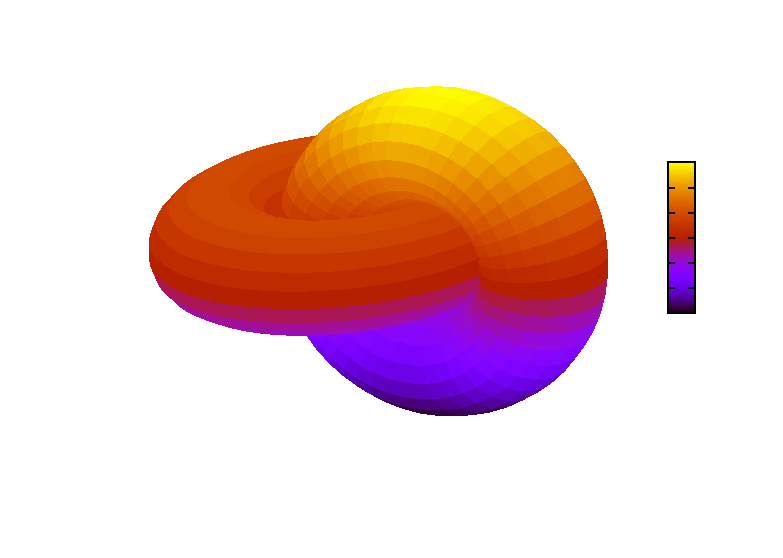
\includegraphics{eg7}}%
    \gplfronttext
  \end{picture}%
\endgroup

  \end{center}
  \caption{Interlocking tori demo, drawn using the epslatex driver.}
  \label{epslatex_test}
}

\begin{figure}[htbp]
  \begin{center}
  % GNUPLOT: LaTeX picture
\setlength{\unitlength}{0.240900pt}
\ifx\plotpoint\undefined\newsavebox{\plotpoint}\fi
\sbox{\plotpoint}{\rule[-0.200pt]{0.400pt}{0.400pt}}%
\begin{picture}(1500,900)(0,0)
\sbox{\plotpoint}{\rule[-0.200pt]{0.400pt}{0.400pt}}%
\put(0.0,0.0){\rule[-0.200pt]{361.109pt}{0.400pt}}
\put(1499.0,0.0){\rule[-0.200pt]{0.400pt}{216.569pt}}
\put(0.0,899.0){\rule[-0.200pt]{361.109pt}{0.400pt}}
\put(0.0,0.0){\rule[-0.200pt]{0.400pt}{216.569pt}}
\put(40,879){\makebox(0,0)[l]{latex  terminal test}}
\put(750.0,0.0){\rule[-0.200pt]{0.400pt}{216.569pt}}
\put(0.0,450.0){\rule[-0.200pt]{361.109pt}{0.400pt}}
\sbox{\plotpoint}{\rule[-0.500pt]{1.000pt}{1.000pt}}%
\multiput(550,470)(20.756,0.000){20}{\usebox{\plotpoint}}
\multiput(950,470)(0.000,-20.756){2}{\usebox{\plotpoint}}
\multiput(950,430)(-20.756,0.000){19}{\usebox{\plotpoint}}
\multiput(550,430)(0.000,20.756){2}{\usebox{\plotpoint}}
\put(550,450){\makebox(0,0)[l]{12345678901234567890}}
\put(550,507){\makebox(0,0)[l]{test of character width:}}
\put(550,470){\usebox{\plotpoint}}
\sbox{\plotpoint}{\rule[-0.200pt]{0.400pt}{0.400pt}}%
\put(750,696){\makebox(0,0)[l]{left justified}}
\put(750,655){\makebox(0,0){centre+d text}}
\put(750,614){\makebox(0,0)[r]{right justified}}
\put(41,450){\makebox(0,0){rotated ce+ntred text}}
\put(123,450){\makebox(0,0)[l]{ rotated by +45 deg}}
\put(82,450){\makebox(0,0)[l]{ rotated by -45 deg}}
\sbox{\plotpoint}{\rule[-0.600pt]{1.200pt}{1.200pt}}%
\put(790.0,880.0){\rule[-0.600pt]{1.200pt}{4.577pt}}
\put(730,840){\makebox(0,0)[r]{show ticscale}}
\put(750.0,860.0){\rule[-0.600pt]{4.818pt}{1.200pt}}
\sbox{\plotpoint}{\rule[-0.200pt]{0.400pt}{0.400pt}}%
\put(1360,859){\makebox(0,0)[r]{-1}}
\put(1380.0,859.0){\rule[-0.200pt]{14.454pt}{0.400pt}}
\put(1360,818){\makebox(0,0)[r]{0}}
\put(1470,818){\rule{1pt}{1pt}}
\put(1380.0,818.0){\rule[-0.200pt]{14.454pt}{0.400pt}}
\put(1360,777){\makebox(0,0)[r]{1}}
\put(1470,777){\makebox(0,0){$+$}}
\put(1380.0,777.0){\rule[-0.200pt]{14.454pt}{0.400pt}}
\put(1360,736){\makebox(0,0)[r]{2}}
\multiput(1380,736)(20.756,0.000){3}{\usebox{\plotpoint}}
\put(1440,736){\usebox{\plotpoint}}
\put(1470,736){\makebox(0,0){$\times$}}
\sbox{\plotpoint}{\rule[-0.400pt]{0.800pt}{0.800pt}}%
\put(1360,695){\makebox(0,0)[r]{3}}
\put(1470,695){\makebox(0,0){$\ast$}}
\put(1380.0,695.0){\rule[-0.400pt]{14.454pt}{0.800pt}}
\sbox{\plotpoint}{\rule[-0.500pt]{1.000pt}{1.000pt}}%
\put(1360,654){\makebox(0,0)[r]{4}}
\multiput(1380,654)(20.756,0.000){3}{\usebox{\plotpoint}}
\put(1440,654){\usebox{\plotpoint}}
\put(1470,654){\raisebox{-.8pt}{\makebox(0,0){$\Box$}}}
\sbox{\plotpoint}{\rule[-0.600pt]{1.200pt}{1.200pt}}%
\put(1360,613){\makebox(0,0)[r]{5}}
\put(1470,613){\makebox(0,0){$\blacksquare$}}
\put(1380.0,613.0){\rule[-0.600pt]{14.454pt}{1.200pt}}
\sbox{\plotpoint}{\rule[-0.500pt]{1.000pt}{1.000pt}}%
\put(1360,572){\makebox(0,0)[r]{6}}
\multiput(1380,572)(41.511,0.000){2}{\usebox{\plotpoint}}
\put(1440,572){\usebox{\plotpoint}}
\put(1470,572){\makebox(0,0){$\circ$}}
\sbox{\plotpoint}{\rule[-0.200pt]{0.400pt}{0.400pt}}%
\put(1360,531){\makebox(0,0)[r]{7}}
\put(1470,531){\makebox(0,0){$\bullet$}}
\put(1380.0,531.0){\rule[-0.200pt]{14.454pt}{0.400pt}}
\put(1360,490){\makebox(0,0)[r]{8}}
\multiput(1380,490)(20.756,0.000){3}{\usebox{\plotpoint}}
\put(1440,490){\usebox{\plotpoint}}
\put(1470,490){\makebox(0,0){$\triangle$}}
\sbox{\plotpoint}{\rule[-0.400pt]{0.800pt}{0.800pt}}%
\put(1360,449){\makebox(0,0)[r]{9}}
\put(1470,449){\makebox(0,0){$\blacktriangle$}}
\put(1380.0,449.0){\rule[-0.400pt]{14.454pt}{0.800pt}}
\sbox{\plotpoint}{\rule[-0.500pt]{1.000pt}{1.000pt}}%
\put(1360,408){\makebox(0,0)[r]{10}}
\multiput(1380,408)(20.756,0.000){3}{\usebox{\plotpoint}}
\put(1440,408){\usebox{\plotpoint}}
\put(1470,408){\makebox(0,0){$\triangledown$}}
\sbox{\plotpoint}{\rule[-0.600pt]{1.200pt}{1.200pt}}%
\put(1360,367){\makebox(0,0)[r]{11}}
\put(1470,367){\makebox(0,0){$\blacktriangledown$}}
\put(1380.0,367.0){\rule[-0.600pt]{14.454pt}{1.200pt}}
\sbox{\plotpoint}{\rule[-0.500pt]{1.000pt}{1.000pt}}%
\put(1360,326){\makebox(0,0)[r]{12}}
\multiput(1380,326)(41.511,0.000){2}{\usebox{\plotpoint}}
\put(1440,326){\usebox{\plotpoint}}
\put(1470,326){\makebox(0,0){$\lozenge$}}
\sbox{\plotpoint}{\rule[-0.200pt]{0.400pt}{0.400pt}}%
\put(1360,285){\makebox(0,0)[r]{13}}
\put(1470,285){\makebox(0,0){$\blacklozenge$}}
\put(1380.0,285.0){\rule[-0.200pt]{14.454pt}{0.400pt}}
\put(1360,244){\makebox(0,0)[r]{14}}
\multiput(1380,244)(20.756,0.000){3}{\usebox{\plotpoint}}
\put(1440,244){\usebox{\plotpoint}}
\put(1470,244){\makebox(0,0){$\heartsuit$}}
\sbox{\plotpoint}{\rule[-0.400pt]{0.800pt}{0.800pt}}%
\put(1360,203){\makebox(0,0)[r]{15}}
\put(1470,203){\makebox(0,0){$\spadesuit$}}
\put(1380.0,203.0){\rule[-0.400pt]{14.454pt}{0.800pt}}
\sbox{\plotpoint}{\rule[-0.500pt]{1.000pt}{1.000pt}}%
\put(1360,162){\makebox(0,0)[r]{16}}
\multiput(1380,162)(20.756,0.000){3}{\usebox{\plotpoint}}
\put(1440,162){\usebox{\plotpoint}}
\put(1470,162){\makebox(0,0){$+$}}
\sbox{\plotpoint}{\rule[-0.600pt]{1.200pt}{1.200pt}}%
\put(1360,121){\makebox(0,0)[r]{17}}
\put(1470,121){\makebox(0,0){$\times$}}
\put(1380.0,121.0){\rule[-0.600pt]{14.454pt}{1.200pt}}
\sbox{\plotpoint}{\rule[-0.500pt]{1.000pt}{1.000pt}}%
\put(1360,80){\makebox(0,0)[r]{18}}
\multiput(1380,80)(41.511,0.000){2}{\usebox{\plotpoint}}
\put(1440,80){\usebox{\plotpoint}}
\put(1470,80){\makebox(0,0){$\ast$}}
\sbox{\plotpoint}{\rule[-0.200pt]{0.400pt}{0.400pt}}%
\put(562,225){\vector(1,0){140}}
\put(562,225){\vector(-1,0){140}}
\put(562,225){\vector(0,1){140}}
\put(562,225){\vector(0,-1){140}}
\put(462,125){\vector(1,1){200}}
\put(462,325){\line(1,-1){100}}
\put(562,225){\vector(1,-1){100}}
\put(262,36){\makebox(0,0)[l]{  lw 1}}
\put(112.0,36.0){\rule[-0.200pt]{36.135pt}{0.400pt}}
\put(262,72){\makebox(0,0)[l]{  lw 2}}
\put(112.0,72.0){\rule[-0.200pt]{36.135pt}{0.400pt}}
\put(262,108){\makebox(0,0)[l]{  lw 3}}
\put(112.0,108.0){\rule[-0.200pt]{36.135pt}{0.400pt}}
\put(262,144){\makebox(0,0)[l]{  lw 4}}
\put(112.0,144.0){\rule[-0.200pt]{36.135pt}{0.400pt}}
\put(262,180){\makebox(0,0)[l]{  lw 5}}
\put(112.0,180.0){\rule[-0.200pt]{36.135pt}{0.400pt}}
\put(262,216){\makebox(0,0)[l]{  lw 6}}
\put(112,252){\makebox(0,0)[l]{linewidth}}
\put(112.0,216.0){\rule[-0.200pt]{36.135pt}{0.400pt}}
\put(1009,173){\makebox(0,0){pattern fill}}
\put(750.0,0.0){\rule[-0.200pt]{0.400pt}{26.981pt}}
\put(750.0,112.0){\rule[-0.200pt]{8.913pt}{0.400pt}}
\put(787.0,0.0){\rule[-0.200pt]{0.400pt}{26.981pt}}
\put(768,132){\makebox(0,0){ 0}}
\put(805,0){\rule{8.9133pt}{26.9808pt}}
\put(750.0,0.0){\rule[-0.200pt]{8.913pt}{0.400pt}}
\put(805.0,0.0){\rule[-0.200pt]{0.400pt}{26.981pt}}
\put(805.0,112.0){\rule[-0.200pt]{8.913pt}{0.400pt}}
\put(842.0,0.0){\rule[-0.200pt]{0.400pt}{26.981pt}}
\put(823,132){\makebox(0,0){ 1}}
\put(805.0,0.0){\rule[-0.200pt]{8.913pt}{0.400pt}}
\put(860.0,0.0){\rule[-0.200pt]{0.400pt}{26.981pt}}
\put(860.0,112.0){\rule[-0.200pt]{8.913pt}{0.400pt}}
\put(897.0,0.0){\rule[-0.200pt]{0.400pt}{26.981pt}}
\put(878,132){\makebox(0,0){ 2}}
\put(915,0){\rule{8.9133pt}{26.9808pt}}
\put(860.0,0.0){\rule[-0.200pt]{8.913pt}{0.400pt}}
\put(915.0,0.0){\rule[-0.200pt]{0.400pt}{26.981pt}}
\put(915.0,112.0){\rule[-0.200pt]{8.913pt}{0.400pt}}
\put(952.0,0.0){\rule[-0.200pt]{0.400pt}{26.981pt}}
\put(933,132){\makebox(0,0){ 3}}
\put(915.0,0.0){\rule[-0.200pt]{8.913pt}{0.400pt}}
\put(970.0,0.0){\rule[-0.200pt]{0.400pt}{26.981pt}}
\put(970.0,112.0){\rule[-0.200pt]{8.913pt}{0.400pt}}
\put(1007.0,0.0){\rule[-0.200pt]{0.400pt}{26.981pt}}
\put(988,132){\makebox(0,0){ 4}}
\put(1025,0){\rule{8.9133pt}{26.9808pt}}
\put(970.0,0.0){\rule[-0.200pt]{8.913pt}{0.400pt}}
\put(1025.0,0.0){\rule[-0.200pt]{0.400pt}{26.981pt}}
\put(1025.0,112.0){\rule[-0.200pt]{8.913pt}{0.400pt}}
\put(1062.0,0.0){\rule[-0.200pt]{0.400pt}{26.981pt}}
\put(1043,132){\makebox(0,0){ 5}}
\put(1025.0,0.0){\rule[-0.200pt]{8.913pt}{0.400pt}}
\put(1080.0,0.0){\rule[-0.200pt]{0.400pt}{26.981pt}}
\put(1080.0,112.0){\rule[-0.200pt]{8.913pt}{0.400pt}}
\put(1117.0,0.0){\rule[-0.200pt]{0.400pt}{26.981pt}}
\put(1098,132){\makebox(0,0){ 6}}
\put(1135,0){\rule{8.9133pt}{26.9808pt}}
\put(1080.0,0.0){\rule[-0.200pt]{8.913pt}{0.400pt}}
\put(1135.0,0.0){\rule[-0.200pt]{0.400pt}{26.981pt}}
\put(1135.0,112.0){\rule[-0.200pt]{8.913pt}{0.400pt}}
\put(1172.0,0.0){\rule[-0.200pt]{0.400pt}{26.981pt}}
\put(1153,132){\makebox(0,0){ 7}}
\put(1135.0,0.0){\rule[-0.200pt]{8.913pt}{0.400pt}}
\put(1190.0,0.0){\rule[-0.200pt]{0.400pt}{26.981pt}}
\put(1190.0,112.0){\rule[-0.200pt]{8.913pt}{0.400pt}}
\put(1227.0,0.0){\rule[-0.200pt]{0.400pt}{26.981pt}}
\put(1208,132){\makebox(0,0){ 8}}
\put(1245,0){\rule{8.9133pt}{26.9808pt}}
\put(1190.0,0.0){\rule[-0.200pt]{8.913pt}{0.400pt}}
\put(1245.0,0.0){\rule[-0.200pt]{0.400pt}{26.981pt}}
\put(1245.0,112.0){\rule[-0.200pt]{8.913pt}{0.400pt}}
\put(1282.0,0.0){\rule[-0.200pt]{0.400pt}{26.981pt}}
\put(1263,132){\makebox(0,0){ 9}}
\put(1245.0,0.0){\rule[-0.200pt]{8.913pt}{0.400pt}}
\put(1050,842){\makebox(0,0){No filled polygons}}
\end{picture}

  \end{center}
  \caption{Line and point types for the basic latex terminal. Note lack of text rotation.}
  \label{testcomp}
\end{figure}

\section{Contact for help}

For general gnuplot questions, you can post to the gnuplot newsgroup 
\url{comp.graphics.apps.gnuplot}.
Additional sources of information are listed on the gnuplot homepage
\url{http://www.gnuplot.info}.

\end{document}
